% Copyright (C) 2014-2020 by Thomas Auzinger <thomas@auzinger.name>

\documentclass[draft,final]{vutinfth} % Remove option 'final' to obtain debug information.

% Load packages to allow in- and output of non-ASCII characters.
\usepackage{lmodern}        % Use an extension of the original Computer Modern font to minimize the use of bitmapped letters.
\usepackage[T1]{fontenc}    % Determines font encoding of the output. Font packages have to be included before this line.
\usepackage[utf8]{inputenc} % Determines encoding of the input. All input files have to use UTF8 encoding.

% Extended LaTeX functionality is enables by including packages with \usepackage{...}.
\usepackage{amsmath}    % Extended typesetting of mathematical expression.
\usepackage{amssymb}    % Provides a multitude of mathematical symbols.
\usepackage{mathtools}  % Further extensions of mathematical typesetting.
\usepackage{microtype}  % Small-scale typographic enhancements.
\usepackage[inline]{enumitem} % User control over the layout of lists (itemize, enumerate, description).
\usepackage{multirow}   % Allows table elements to span several rows.
\usepackage{booktabs}   % Improves the typesettings of tables.
\usepackage{subcaption} % Allows the use of subfigures and enables their referencing.
\usepackage[ruled,linesnumbered,algochapter]{algorithm2e} % Enables the writing of pseudo code.
\usepackage[usenames,dvipsnames,table]{xcolor} % Allows the definition and use of colors. This package has to be included before tikz.
\usepackage{nag}       % Issues warnings when best practices in writing LaTeX documents are violated.
\usepackage{todonotes} % Provides tooltip-like todo notes.
\usepackage{hyperref}  % Enables cross linking in the electronic document version. This package has to be included second to last.
\usepackage[acronym,toc]{glossaries} % Enables the generation of glossaries and lists fo acronyms. This package has to be included last.

\usepackage{graphicx}% enables cropping of images
\usepackage{datetime2}
\usepackage{array}
\newcolumntype{L}[1]{>{\raggedright\let\newline\\\arraybackslash\hspace{0pt}}m{#1}}
\newcolumntype{C}[1]{>{\centering\let\newline\\\arraybackslash\hspace{0pt}}m{#1}}
\newcolumntype{R}[1]{>{\raggedleft\let\newline\\\arraybackslash\hspace{0pt}}m{#1}}

%enable code block with syntax highlighting
\usepackage{listings}
\usepackage{xcolor}
\usepackage{bera}% optional: just to have a nice mono-spaced font
\usepackage{upquote}

\definecolor{codegreen}{rgb}{0,0.6,0}
\definecolor{codegray}{rgb}{0.5,0.5,0.5}
\definecolor{codepurple}{rgb}{0.58,0,0.82}
\definecolor{backcolour}{rgb}{0.95,0.95,0.92}

\colorlet{punct}{red!60!black}
\definecolor{background}{HTML}{EEEEEE}
\definecolor{delim}{RGB}{20,105,176}
\colorlet{numb}{magenta!60!black}

\lstdefinelanguage{json}{
    basicstyle=\small\ttfamily,
    numbers=left,
    numberstyle=\scriptsize,
    stepnumber=1,
    numbersep=8pt,
    showstringspaces=false,
    breaklines=true,
    frame=lines,
    backgroundcolor=\color{background},
    literate=
     *{0}{{{\color{numb}0}}}{1}
      {1}{{{\color{numb}1}}}{1}
      {2}{{{\color{numb}2}}}{1}
      {3}{{{\color{numb}3}}}{1}
      {4}{{{\color{numb}4}}}{1}
      {5}{{{\color{numb}5}}}{1}
      {6}{{{\color{numb}6}}}{1}
      {7}{{{\color{numb}7}}}{1}
      {8}{{{\color{numb}8}}}{1}
      {9}{{{\color{numb}9}}}{1}
      {:}{{{\color{punct}{:}}}}{1}
      {,}{{{\color{punct}{,}}}}{1}
      {\{}{{{\color{delim}{\{}}}}{1}
      {\}}{{{\color{delim}{\}}}}}{1}
      {[}{{{\color{delim}{[}}}}{1}
      {]}{{{\color{delim}{]}}}}{1},
}

\definecolor{editorGray}{rgb}{0.95, 0.95, 0.95}
\definecolor{editorOcher}{rgb}{1, 0.5, 0} % #FF7F00 -> rgb(239, 169, 0)
\definecolor{editorGreen}{rgb}{0, 0.5, 0} % #007C00 -> rgb(0, 124, 0)

\lstdefinelanguage{HTML5}{
        language=html,
        sensitive=true, 
        alsoletter={<>=-},
        otherkeywords={
        % HTML tags
        <html>, <head>, <title>, </title>, <meta, />, </head>, <body>,
        <canvas, \/canvas>, <script>, </script>, </body>, </html>, <!, html>, <style>, </style>, ><,
        <a-scene, </a-scene>, <a-entity, </a-entity>, <a-text, </a-text>, \ >
        },   
        ndkeywords={
        % General
        =,
        % HTML attributes
        charset=, id=, width=, height=,
        % CSS properties
        border:, transform:, -moz-transform:, transition-duration:, transition-property:, transition-timing-function:
        }, 
        morecomment=[s]{<!--}{-->},
        tag=[s]
}

\lstdefinelanguage{JavaScript}{
  keywords={typeof, new, true, false, catch, function, return, null, catch, switch, var, if, in, while, do, else, case, break},
  keywordstyle=\color{blue}\bfseries,
  ndkeywords={class, export, boolean, throw, implements, import, this, const, let},
  ndkeywordstyle=\color{darkgray}\bfseries,
  identifierstyle=\color{black},
  sensitive=false,
  comment=[l]{//},
  morecomment=[s]{/*}{*/},
  commentstyle=\color{purple}\ttfamily,
  stringstyle=\color{red}\ttfamily,
  morestring=[b]',
  morestring=[b]"
}


\lstset{%
    % Basic design
    backgroundcolor=\color{background},
    basicstyle=\small\ttfamily,   
    frame=lines,
    % Line numbers
    xleftmargin={0.75cm},
    numbers=left,
    numberstyle=\scriptsize,
    stepnumber=1,
    numbersep=8pt,
    firstnumber=1,
    numberfirstline=true,
    % Code design   
    keywordstyle=\color{blue}\bfseries,
    commentstyle=\color{darkgray}\ttfamily,
    ndkeywordstyle=\color{editorGreen}\bfseries,
    stringstyle=\color{editorOcher},
    % Code
    language=HTML5,
    alsodigit={.:;},
    tabsize=2,
    showtabs=false,
    showspaces=false,
    showstringspaces=false,
    extendedchars=true,
    breaklines=true,        
    % Support for German umlauts
    literate=%
    {Ö}{{\"O}}1
    {Ä}{{\"A}}1
    {Ü}{{\"U}}1
    {ß}{{\ss}}1
    {ü}{{\"u}}1
    {ä}{{\"a}}1
    {ö}{{\"o}}1
}

% Define convenience functions to use the author name and the thesis title in the PDF document properties.
\newcommand{\authorname}{Manuel Eiweck} % The author name without titles.
\newcommand{\thesistitle}{Immersive 3D Multilayer Graph} % The title of the thesis. The English version should be used, if it exists.

% Set PDF document properties
\hypersetup{
    pdfpagelayout   = TwoPageRight,           % How the document is shown in PDF viewers (optional).
    linkbordercolor = {Melon},                % The color of the borders of boxes around crosslinks (optional).
    pdfauthor       = {\authorname},          % The author's name in the document properties (optional).
    pdftitle        = {\thesistitle},         % The document's title in the document properties (optional).
    pdfsubject      = {Subject},              % The document's subject in the document properties (optional).
    pdfkeywords     = {a, list, of, keywords} % The document's keywords in the document properties (optional).
}

\setpnumwidth{2.5em}        % Avoid overfull hboxes in the table of contents (see memoir manual).
\setsecnumdepth{subsection} % Enumerate subsections.

\nonzeroparskip             % Create space between paragraphs (optional).
\setlength{\parindent}{0pt} % Remove paragraph identation (optional).

\makeindex      % Use an optional index.
\makeglossaries % Use an optional glossary.
%\glstocfalse   % Remove the glossaries from the table of contents.

% Set persons with 4 arguments:
%  {title before name}{name}{title after name}{gender}
%  where both titles are optional (i.e. can be given as empty brackets {}).
\setauthor{}{\authorname}{}{male}
\setadvisor{Univ.Ass. Dr.techn.}{Manuela Waldner}{MSc.}{female}

% For bachelor and master theses:  
\setfirstassistant{Dipl.-Ing. Dr.techn.}{Johannes Sorger}{}{male}
\setsecondassistant{Dipl.-Ing.}{Wolfgang Knecht}{}{male}
%\setthirdassistant{Pretitle}{Forename Surname}{Posttitle}{male}

% For dissertations:
\setfirstreviewer{Pretitle}{Forename Surname}{Posttitle}{male}
\setsecondreviewer{Pretitle}{Forename Surname}{Posttitle}{male}

% For dissertations at the PhD School and optionally for dissertations:
\setsecondadvisor{Pretitle}{Forename Surname}{Posttitle}{male} % Comment to remove.

% Required data.
\setregnumber{01633012}
\setdate{01}{01}{2001} % Set date with 3 arguments: {day}{month}{year}.
\settitle{\thesistitle}{Immersive 3D Multilayer Graph} % Sets English and German version of the title (both can be English or German). If your title contains commas, enclose it with additional curvy brackets (i.e., {{your title}}) or define it as a macro as done with \thesistitle.
\setsubtitle{Three-dimensional	multilayer visualization approach for hierarchical networks in VR}{Three-dimensional	multilayer visualization approach for hierarchical networks in VR} % Sets English and German version of the subtitle (both can be English or German).

% Select the thesis type: bachelor / master / doctor / phd-school.
% Bachelor:
\setthesis{bachelor}
%
% Master:
%\setthesis{master}
%\setmasterdegree{dipl.} % dipl. / rer.nat. / rer.soc.oec. / master
%
% Doctor:
%\setthesis{doctor}
%\setdoctordegree{rer.soc.oec.}% rer.nat. / techn. / rer.soc.oec.
%
% Doctor at the PhD School
%\setthesis{phd-school} % Deactivate non-English title pages (see below)

% For bachelor and master:
\setcurriculum{Media Informatics and Visual Computing}{Medieninformatik und Visual Computing} % Sets the English and German name of the curriculum.

% For dissertations at the PhD School:
\setfirstreviewerdata{Affiliation, Country}
\setsecondreviewerdata{Affiliation, Country}


\begin{document}

\frontmatter % Switches to roman numbering.
% The structure of the thesis has to conform to the guidelines at
%  https://informatics.tuwien.ac.at/study-services

%Place this before begin document 
%\usepackage{datetime2}
%\usepackage{array}
%\newcolumntype{L}[1]{>{\raggedright\let\newline\\\arraybackslash\hspace{0pt}}m{#1}}
%\newcolumntype{C}[1]{>{\centering\let\newline\\\arraybackslash\hspace{0pt}}m{#1}}
%\newcolumntype{R}[1]{>{\raggedleft\let\newline\\\arraybackslash\hspace{0pt}}m{#1}}

This Document is not finished yet and currently in development.\\
\\
version: 0.6.1\\
created on: \DTMnow\\
\\
\textbf{Version History:}\\

\begin{tabularx}{\textwidth} { | c | c | L{9.493cm} | }
    \hline
    \textbf{Version} & \textbf{Release date} &\textbf{Notes} \\
    \hline
    0.1.1 & 16.12.20 & thesis structure, background and related work paper \\
    \hline
    0.2.1 & 21.12.20 & first draft chapter 1 introduction \\
    \hline
    0.3.1 & 07.01.21 & rework abstract and introduction, first draft background\\
    \hline
    0.3.2 & 18.01.21 & rework abstract, introduction and background. Change paper and structure of related work\\
    \hline
    0.4.1 & 22.01.21 & first draft related work\\
    \hline
    0.5.1 & 01.02.21 & rework related work, first draft proposed solution \\
    \hline
    0.5.2 & 05.02.21 & rework introduction and proposed solution\\
    \hline
    0.6.1 & 24.02.21 & rework proposed solution, first draft implementation\\
    \hline
 \end{tabularx}%remove this line when releasing the document 

\addtitlepage{naustrian} % German title page (not for dissertations at the PhD School).
\addtitlepage{english} % English title page.
\addstatementpage

\begin{danksagung*}
    Einen besonderen Dank möchte ich den Betreuern dieser Arbeit Johannes Sorger, Wolfgang Knecht sowie Manuela Waldner aussprechen welche mich in der Entwicklungsphase dieser Bachelorarbeit tatkräftig unterstützt haben.
Weiters gilt mein Dank ebenfalls meinen Freunden Thomas Jakli und Lars Müller welche mir Feedback zur implementierten Visualisierung gegeben sowie beim Erstellen der Präsentations Website geholfen haben.
Außerdem möchte ich mich bei all meinen Studienkollegen und Studienkolleginnen im speziellen Pascal Hann und Aaron Wedral bedanken, ohne denen mein Studium sicherlich nicht so erfolgreich und unterhaltsam gewesen wäre. 
Zu guter Letzt bedanke ich mich bei meinen Eltern sowie meiner Schwester für die großartige Unterstützung in all diesen Jahren. 
\end{danksagung*}

%\begin{acknowledgements*}
%    Acknowledgments
 
%\end{acknowledgements*}

\begin{kurzfassung}
    Kurzfassung 
\end{kurzfassung}

\begin{abstract}
    Our world is becoming more digital each year, new parts of our daily life getting connected and the amount and complexity of the produced data increases steadily.
The analysis of this data enables big opportunities for science and industry.
A subset of this data is organized in the form of hierarchical networks. We see this in multiple application domains for example medical research where connections, group and cluster memberships of diseases are tracked; Social science where relationships are mapped in company organization charts; In software engineering in the form of build-, dependency- and source code version management software with hierarchical connections between software modules, versions and layered software architecture.

However, getting insight into this complex data with traditional two-dimensional visualization is getting more difficult as the visual clutter increases significantly with the exponentially growth of data we saw in recent years. Therefore, we need new methods and techniques to facilitate and expedite the analysis process.
In this thesis, we investigate a new approach to visualize hierarchical network data by extending already existing concepts of two-dimensional hierarchical network visualizations with a third dimension and applying it to a virtual reality based visualization system. We believe that the capabilities of virtual reality devices, such as improved spatial impression and interaction possibilities by room-scale tracked headsets and controllers allow the visualization to fully utilize the benefits of three-dimensional information visualization. Therefore, it should be possible to analyze even bigger and more complex hierarchical networks than currently possible with conventional two-dimensional visualizations. 
\end{abstract}

% Select the language of the thesis, e.g., english or naustrian.
\selectlanguage{english}

% Add a table of contents (toc).
\tableofcontents % Starred version, i.e., \tableofcontents*, removes the self-entry.

% Switch to arabic numbering and start the enumeration of chapters in the table of content.
\mainmatter

\chapter{Introduction}

\section{Motivation}
Revealing the structure of hierarchical organized data is a complex task where many approaches already exists. It is still an active research area as data scientists are facing ever greater challenges when analyzing large hierarchical datasets. One example is the Human Disease Network \cite{zhou_human_2014} which is a hierarchical network of disorders and disease genes with approximately 3000 nodes on two different hierarchy layers. Figure \ref{fig:Human_Disease_Network} shows us the representation of the data in a common two-dimensional layout. In this representation, the classes of disorders are coded by color. 
Another dataset with a similar structure can be seen in Figure \ref{fig:original2DdiseaseNet}, here the clusters of different diseases are grouped by boxes.\\ 
Depiction of hierarchical network structure in 2D faces us with many challenges. The biggest one is visual clutter also called hairball effect which reduces the legibility of the network information, therefore it is difficult to determine node-node relationships and hierarchic-associations as well as hierarchic relationships which are crucial in analyzing hierarchical network data. In Figure \ref{fig:Human_Disease_Network} we can see this effect on the green nodes. The graph in Figure \ref{fig:original2DdiseaseNet} solves this problem by hiding links between child nodes from different boxes which is also not optimal.

\begin{figure}[h]
    \centering
    \begin{subfigure}[b]{0.4\columnwidth}
        \centering
        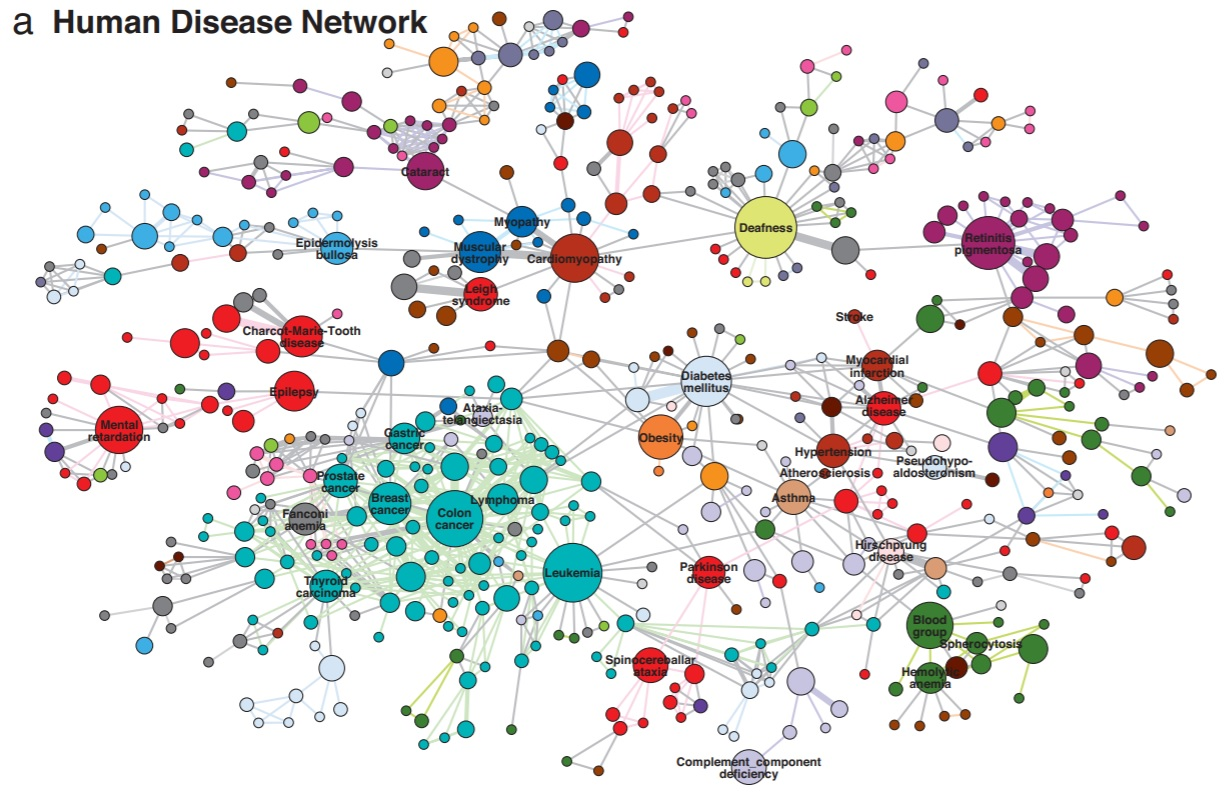
\includegraphics[width=\textwidth, trim={0 0 9cm 0},clip]{graphics/Human_Disease_Network.jpg}
        \subcaption{Human Disease Network \cite{zhou_human_2014}}
        \label{fig:Human_Disease_Network}
    \end{subfigure}
    \begin{subfigure}[b]{0.5\columnwidth}
      \centering
      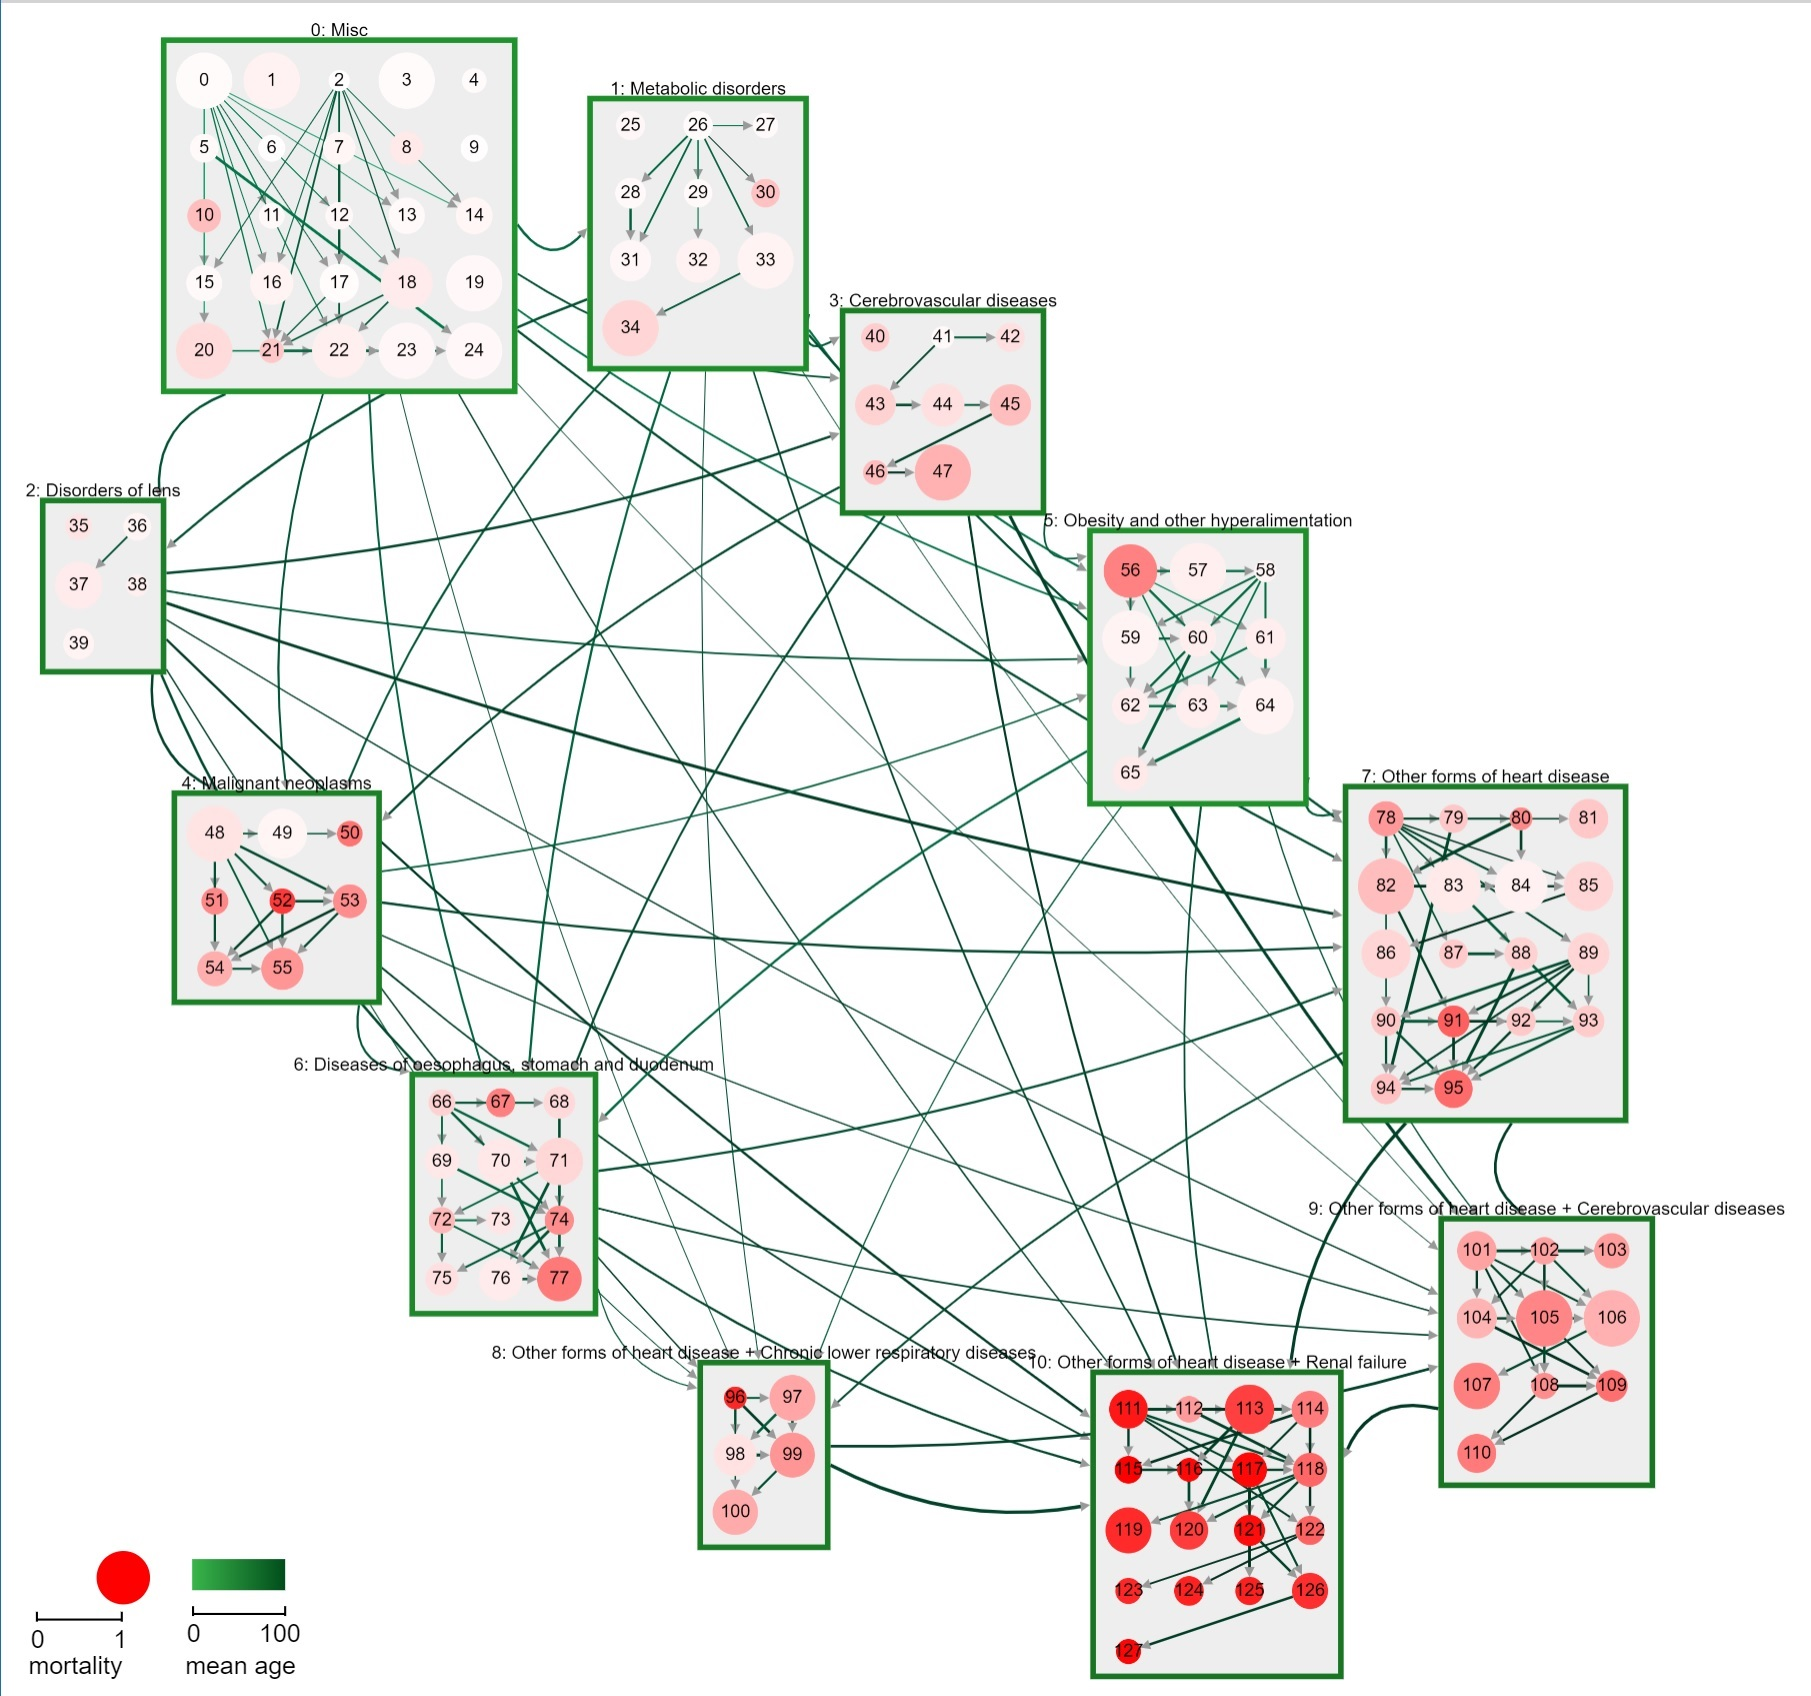
\includegraphics[width=\textwidth]{graphics/original2DdiseaseNet.jpg}
      \subcaption{a comorbidity network of diagnoses related to diabetes melitus}
      \label{fig:original2DdiseaseNet}
    \end{subfigure}
    \caption[Optional caption for the figure list (often used to abbreviate long captions)]{Example visualizations of hierarchical network datasets in two dimensions. Both consists of two hierarchical layers.} % Remove the [...] argument if the original caption should be used in the figure list.
    \label{fig:intro} 
  \end{figure}

3D information visualization allows us to expand the user experience of traditional 2D graphs. As Brath describes in his paper \cite{brath_3d_2014} there are many advantages and opportunities when using three-dimensional visualizations.
By using an additional axis the visualization has more space to distribute all the data and reduce clutter in the first place before applying specialized layouts. The mental model of the data gets improved which leads to a better cluster detection, conformation and general overview of the data. 
Some visualization also use the additional axis to encode an extra attribute by its position, this can be seen in the “3D space time cube” \cite{brath_3d_2014} here the temporal information is encoded on the Z axis another common usage is a 3D scatter plot.
In three-dimensional layouts, the perspective of the visualization has to be reconsidered. Usually the user looks from the outside with a bird's eye view at the visualization. In 3D however the viewer can be placed right inside our graph, this enables us to utilize new navigation and interaction possibilities.

Still, all these opportunities also involve new challenges: navigation inside a hierarchically structured 3D scene, occlusion of elements in an 3D perspective view, selection of objects for displaying details and the lack of a reference point in an abstract three-dimensional space. Brath \cite{brath_3d_2014} already stated that immersive interfaces could help to overcome these issues.\label{chap:advantages_VR}
We believe that the recent developments in virtual reality hardware and frameworks offer great potential to address these challenges. 
We can see the benefits of VR based visualizations in various publications. Bowman et al. \cite{bowman_virtual_2007} examined the impact of VR techniques, like stereoscopic images, interaction with the virtual world and head movement, can have on users. 
Recently Kraus et al. \cite{kraus_impact_2020} did a study on the effect of immersion for detecting clusters in a scatter plot. Their results show that VR based visualization systems have real world advantages in terms of time needed to get an overview of the data compared to traditional 2D- and 3D information visualization. 
 
\section{Aim of the Work}

Our goal is to implement a visualization for hierarchical network data that allows users take the benefits of 3D information visualization and opportunities of virtual reality technology to dive right into the data. We believe the combination of both concepts complement each other well because VR based technology can be used to solve the subsequent challenges from 3D information visualization and therefore enable data scientists to optimize their data analysis tasks. 
Our aim was to design a customized graph layout that calculates the position and size of each node by the hierarchical structure: child nodes are nested within their parent node. 
In addition, visual clutter by overlapping of nodes and links should be prevented. 
Furthermore, the exploration of the resulting graph should be possible with room scale virtual reality devices like the HTC Vive, requiring optimized navigation, filtering and brushing methods to enhance the graph exploration user experience.

\section{Methodology}
In order to achieve the proclaimed goal we firstly did research on already working solutions. We summarized important techniques many approaches share and categorized them into different visualization types in Section \ref{chap:rw-2d3dLayout}. 
Before improving a visualization we had to get a clear understanding of our data structure, therefore we looked into the theory behind it. Section \ref{chap:bg-graphTheory} explains the concepts of different graphs data structures, their extensions like trees but also fundamentally drawing techniques like node-link diagrams.
As we were planning a VR visualization, we also looked into VR technology from a feature perspective in Section \ref{chap:bg-vrtech}. Furthermore, we examined other related works in the field of VR visualization including navigation and interaction methods as well as VR specialized graph layouts in Section \ref{chap:rw-VRVIS}.\\
With our goal in mind we defined some requirements the visualization has to meet in order to be a success. These requirements including a summary how we planned to fulfilled them can be found in Section \ref{chap:ps-requirements}. 
To design our own visualization system we need a concept for our VR specialized layout which can be found in Section \ref{chap:ps-layout}. 
Its task is to find the node positions in order to achieve a distributed hierarchical nested graph with no node overlapping, which is primarily done by a customized force system.
Furthermore, a fitting render representation had been designed (see Section \ref{chap:ps-graphRepresentation}) as well as VR optimized interaction (see Section \ref{chap:solution-interaction}) and navigation methods (see Section \ref{chap:solution-navigation}). 
A detail description on the implementation process can be found in Chapter \ref{chap:Impl}. The resulting visualization can be seen in Figure \ref{fig:conceptSketch}.\\
For evaluation, we measured performance and technical limits of our solution in Section (TODO). In addition, we did multiple informational feedback interviews and documented the results as well as if the solution met all the requirements in Section (TODO). As a side note, due to the COVID-19 pandemic during the writing we had restrictions on gathering feedback therefore we got a reduced set of people testing out our visualization.\\
Lastly in Chapter (TODO) we discuss some problems and possible future work.

\begin{figure}[h]
    \centering
    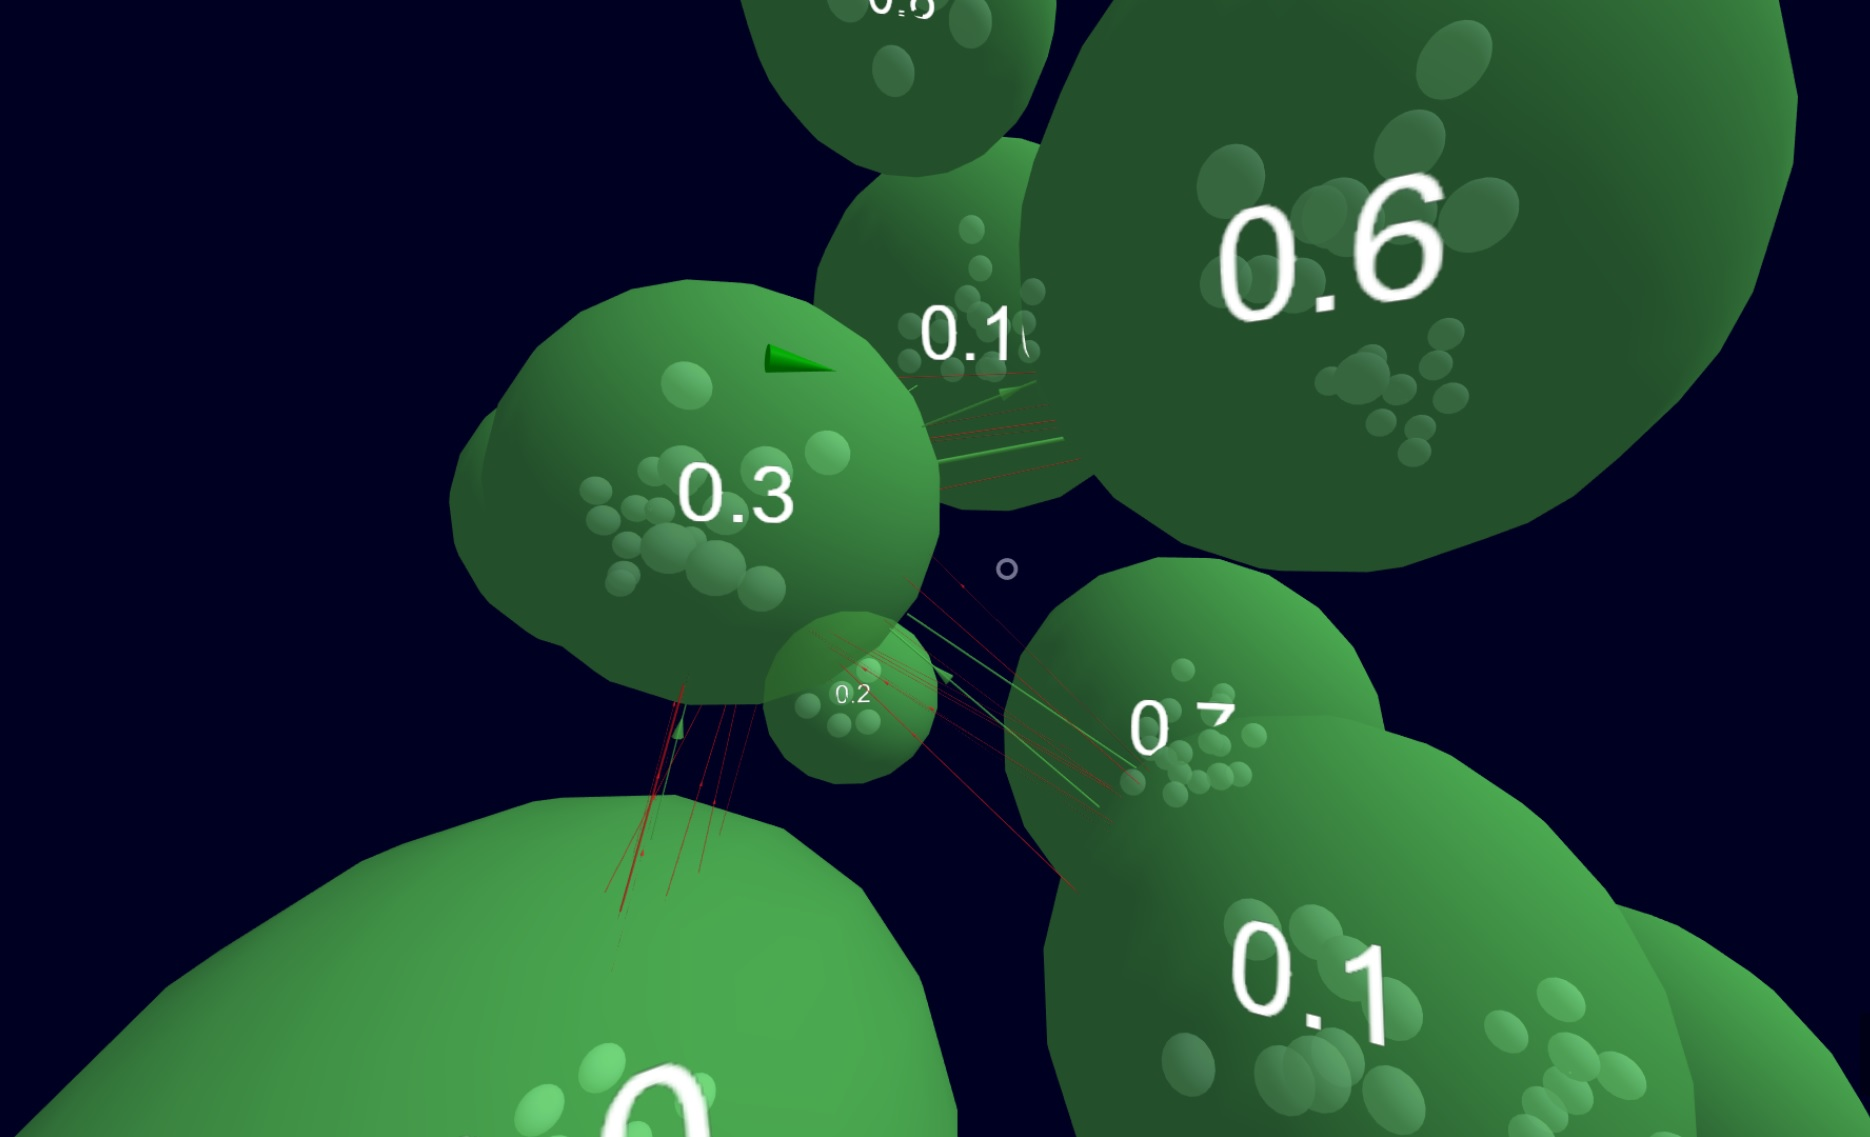
\includegraphics[width=1\textwidth]{graphics/conceptScreenshot.jpg}
    \caption{Screenshot of the comorbidity network dataset from \ref{fig:original2DdiseaseNet} in our hierarchical network visualization. On the screenshot only edges from node 0.3 are displayed.} % Remove the [...] argument if the original caption should be used in the figure list.
    \label{fig:conceptSketch} 
\end{figure}

\chapter{Background}

\section{Graph Theory}

Before we begin discussing different visualization techniques, it is important to understand the data behind the visualization. As we are not limiting ourselves to a specific application domain, the key is to understand the structure of the data. Simply speaking we are dealing with graph or network data, but as there are multiple terms and terminologies used we want to give a short summary. 

In general, a graph consists of vertices and edges \cite{diestel_graph_2017}. In the context of this thesis we also use the terms nodes for vertices, links for edges and network for graph interchangeably. Furthermore, edges in a graph can either be directed or undirected. Directed edges differentiate between source and target node where undirected edges do not. Additionally, we also distinguish between weighted and unweighted edges. Weighted edges have any sort of numerical comparable attribute. This can be used for instance to describe how strong the relation between nodes is. Figure \ref{fig:simple_weighted_directed_network} shows a directed and weighted graph.

A specialized version of a graph is called tree. It is defined as an acyclic graph where all subcomponents of the graph are connected \cite{diestel_graph_2017}. One node of the tree can be picked as a root node which is usually drawn on the top. Nodes with only one link are called leaf nodes and drawn on the bottom, see Figure \ref{fig:simple_tree}.\\
In addition, tree nodes also have a height and depth. The height is defined by the largest number of edges between the root node and a leaf node. The height of the root node is the height of the tree itself. The dept of the node is the number of edges along the path to the root node. Note that a tree is able to encode hierarchical relationships between nodes. In the thesis we use the term 'hierarchical level' for depth and terminologies like 'leaf1 is a direct child of node1' or 'node1 is the parent (node) of leaf1' based on Figure \ref{fig:simple_tree}.

In addition to the basic graph structures, which are often not sufficient for specific datasets, there are extended forms of graph models \cite{bertault_algorithm_1999}. 
%higraph, clustered graph, compound graph
For the context of this thesis, clustered graphs are especially interesting. A clustered graph is defined by a recursive structure where each node can be new graph for itself \cite{eades_multilevel_1997}.\\ 
%Another would be a compound graph. a set of different elements such as vertices or edges and therefore 
%compound graph (master thesis), 
Furthermore, multivariate networks \cite{kerren_introduction_2014} combines the data type of network with multidimensional datasets. Each node and edge can have numerous additional attributes these can be numerical, ordinal or categorical.

\begin{figure}[h]
    \centering
    \begin{subfigure}[b]{0.45\columnwidth}
        \centering
        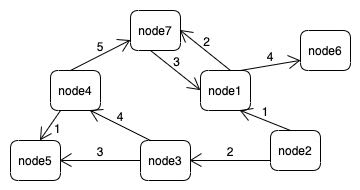
\includegraphics[width=\textwidth]{graphics/weightedDirectedNetwork.jpg}
        \subcaption{Weighted and directed graph.}
        \label{fig:simple_weighted_directed_network}
    \end{subfigure}
    \begin{subfigure}[b]{0.54\columnwidth}
        \centering
        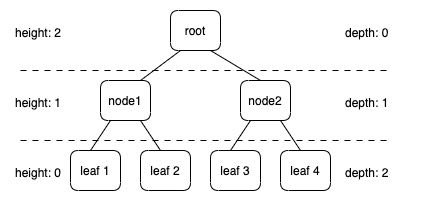
\includegraphics[width=\textwidth]{graphics/basicTree.jpg}
        \subcaption{Tree with a height of 2.}
        \label{fig:simple_tree}
    \end{subfigure}
    
    \caption[Optional caption for the figure list (often used to abbreviate long captions)]{Simple visualizations of graph data structures} % Remove the [...] argument if the original caption should be used in the figure list.
    \label{fig:intro} 
  \end{figure}

In conclusion, the most basic graph or network would be a simple unweighted and undirected set of nodes and links without any hierarchical relationship. To be able to represent different types of relationships in our data their exists different extensions. 

\subsection{Graph Drawing}

As graph drawing is a subarea of information visualization, common knowledge from this research area can be applied here as well. With Shneiderman's visual information seeking mantra “Overview first, zoom and filter, then details-on-demand” being one of the most famous \cite{shneiderman_eyes_1996}. Additionally, the Gestalt Principles can also be used in graph drawing as Kobourov et al.
\cite{kobourov_gestalt_2015} shows us. They can be used to produce more aesthetically pleasing visualizations by defining drawing conventions and even improve the impression of the data. Cluster affiliation of nodes can be expressed by similar colors, shapes or simply by proximity. While the form of links should be consistent without any sharp bends.

For representation node-link and space-filling concepts are the most important for the data structures used in this thesis. Space-filling visualizations usually use multiscale approaches to encode hierarchical information. Node-link graphs tend to utilize force-based or constraint-based layouts\cite{von_landesberger_visual_2011}.

Force based layout techniques work without any domain-specific knowledge, therefore provide a flexible way to determine layouts for node link graphs \cite{kobourov_spring_2012}. Only structural information about the graph relationships themselves are used. 
There are a variety of different approaches but concept is always the same. 
These systems work by providing numerous forces between nodes and links, whose job is to update the position of the nodes. Usually these forces are related to Hooke's law, a simple approach by Kamada et al. \cite{kamada_algorithm_1989} is to use repulsive forces between all nodes and attraction forces for linked nodes.
The defined forces are then processed with a given set of nodes and links for either a limited number of iterations, a fixed time, some sort of dynamic condition like the momentum of the nodes fall below a certain threshold or just infinitely.
Large graphs however are a common problem as physical force models tend to have many local minima and therefore not produce optimal results \cite{kobourov_spring_2012}.

\section{Visualization Techniques}
Papers:\\

Shneiderman\\
The Eyes Have It: A Task by Data Type Taxonomy for Information Visualizations\\
Visual Information Seeking Mantra\\
\\
Kobourov\\
Gestalt Principles in Graph Drawing\\
\\
Brath \\
3D InfoVis is Here to Stay: Deal with It\\
Warum allgemein 3D Infos Vis Vorteile hat\\
\\
Lee\\
Task Taxonomy for Graph Visualization\\
a list of tasks for graph visualization that has
enough detail and specificity to be useful to: 1) designers who
want to improve their system and 2) to evaluators who want to
compare graph visualization systems.\\
\\

\subsection{Force-directed graph drawing}
alt:\\
Fruchterman\\
Graph drawing by force-directed placement\\
\\
Kamada Kawai\\
AN ALGORITHM FOR DRAWING GENERAL UNDIRECTED GRAPHS\\
\\

aktueller:\\
Yifan Hu\\
Efficient, High-Quality Force-Directed Graph Drawing\\
Algorithmus für force Graph,  Erklärkung barnes hut etc Sehr detailliert, viel info\\
\\
Kobourov\\
Spring Embedders and Force Directed Graph Drawing Algorithms\\
Mehrere Algorithmen für Force Graph, Sehr detailliert\\
\\

\section{Network Visualization}

\subsection{Network Visualization Basics}

Kerren\\
\textbf{Introduction to Multivariate Network Visualization vorallem Chapter9: Heterogeneous Networks on Multiple Levels} \\
gute Zusammenfassung von Multilayer Network Visualization\\

West\\
Introduction to graph theory\\
\\


\section{VR Technology}

Content:
\begin{itemize}
    \item Describe the technologie stack (OpenVR, WEBXR/WEBVR, A-Frame, ThreeJS)
    \item Devices, HTC-VIVE, Oculus-Rift, Vendors
    \item Room scale vs Table vs Standing, possibilities of tracking
    \item 6 DOF vs 3 DOF (degrees of freedom)
    \item Vergleich HMD zu früheren Möglichkeiten mit "Cave" Virtual Reality
\end{itemize}

official Specs / Docs: 
\\
Desktop API:\\
https://www.khronos.org/openxr/ \\
https://github.com/ValveSoftware/openvr \\
\\
Web API:\\
   WebXR\\
https://immersiveweb.dev/ \\
https://github.com/immersive-web/webxr/blob/master/explainer.md \\
https://immersive-web.github.io/webxr/ \\
https://blog.mozvr.com/webxr-emulator-extension/ \\
\\
WebVR:(deprecated wird aber von unserer AFrame Version verwendet daher trotzdem relevant)\\
https://webvr.info/ \\
\\
Papers:\\
Cruz-Neira\\
The CAVE: audio visual experience automatic virtual environment\\
\\
M Cordeil\\
Immersive Collaborative Analysis of Network Connectivity: CAVE-style or Head-Mounted Display?\\
\\

\chapter{Related Work}



\section{Graph Visualizations}

\subsection{Layout}
\subsubsection{Approaches}
Content:
\begin{itemize}
    \item 2D Layout
    \item 3D Layout 
    \item special VR Layouts 
\end{itemize}
Papers:\\
\\
2D Layout:\\
TODO
\\
\\
3D Layout:\\
TODO
\\
\\
VR Layout:\\
Kwon\\
A Study of Layout, Rendering, and Interaction Methods for Immersive Graph Visualization\\

\subsubsection{Force based}
Content:
\begin{itemize}
    \item Force Algorithmen and concepts 
\end{itemize}
Papers:\\
\\
Kobourov\\
Spring Embedders and Force Directed Graph Drawing Algorithms\\
In this survey we consider several classical algorithms \dots for large and dynamic graphs\\

Jacom\\
ForceAtlas2, a Continuous Graph Layout Algorithm for Handy Network Visualization Designed for the Gephi Software\\
Forcetlas2 is a force-directed layout close to other algorithms used for network spatialization. Integrate different techniques.\\
\\



\subsection{Multilayer Visualization}
Ghonie McGee\\
The State of the Art in Multilayer Network Visualization\\
\\
De Domenico\\
MuxViz: a tool for multilayer analysis and visualization of networks\\
We demonstrate the ability of muxViz to analyse and interactively visualize multilayer data using empirical genetic, neuronal and transportation networks https://github.com/manlius/muxViz\\
\\

\subsection{Hierarchical Visualization}
Nobre\\
The State of the Art in Visualizing Multivariate Networks\\
\\
Shi\\
Hierarchical Focus+Context Heterogeneous Network Visualization\\
OnionGraph, aggregated based on node attributes or network topology,
best of both worlds.\\
\\
Jonker\\
Graph mapping: Multi-scale community visualization of massive graph data\\
\\
Balzer\\
Hierarchy Based 3D Visualization of Large Software Structures\\
\\
Holten\\
Hierarchical Edge Bundles: Visualization of Adjacency Relations in Hierarchical Data\\
\\
Itoh\\
Hierarchical data visualization using a fast rectangle-packing algorithm\\
\\
Munzner\\
H3: laying out large directed graphs in 3D hyperbolic space\\
\\
Mansmann\\
Exploring OLAP aggregates with hierarchical visualization techniques\\
\\

\section{VR Visualizations}

Sorger\\
Immersive Analytics of Large Dynamic Networks via Overview and Detail Navigation\\
Orig Paper https://vis.csh.ac.at/vrnetexplorer/\\
\\
Kwon\\
A Study of Layout, Rendering, and Interaction Methods for Immersive Graph Visualization\\
considerations of layout, rendering, and interaction methods for visualizing graphs in an  immersive environment user study to evaluate our techniques\\
Strat: The viewer is placed at the center of the sphere, on which the graph is laid out.\\
\\
Büschel\\
Augmented Reality Graph Visualizations\\
We present an exploration of the design space for edge styles and discuss the results of a user study comparing six different edge variants.\\
\\
Yang\\
Embodied Navigation in Immersive Abstract Data Visualization:
Is Overview+Detail or Zooming Better for 3D Scatterplot\\

\subsection{Advantages of Visualization in VR}
Kraus\\
The Impact of Immersion on Cluster Identification Tasks\\
quantitative user study to investigate the impact of immersion on cluster identification tasks in scatterplot visualizations\\
\\

\subsection{Navigation}
Content:
\begin{itemize}
    \item "Minimap" in VR
    \item Scaling
    \item Room scale vs Table vs Seating
    \item Overview + Detail 
\end{itemize}

Papers: \\

\subsection{Interaction}
Content: 
\begin{itemize}
    \item Edge Filtering
    \item Raycast/Laserpointer Selection
\end{itemize}

\section{Application and Libraries}
References: https://neo4j.com/developer/tools-graph-visualization/

\subsection{Applications}
Software\\
Gephi\\
\\
Software\\
Neo4j Bloom\\
\subsection{Libraries}
Bostock\\
D3: Data-Driven Documents\\
Examples\\
\\
Software\\
http://www.popotojs.com/ \\
\\
Software\\
https://visjs.org/

\chapter{Proposed Solution}
\label{chap:proposed-Solution}

Our initial motivation for this thesis was to enable visualization of hierarchical and disjoint grouped datasets in VR. 
Data scientists often deal with these datasets and because of the complexity of the data they often have to rely on classical 2D visualization software.
However, current 2D approaches quickly reach their limits and run into the problem of visual clutter, especially when visualizing large networks and deep hierarchies. For example the network shown in Figure \ref{fig:2dHierarchicalClutter} reaches a critical point in visual clutter. The comorbidity network shown in Figure \ref{fig:original2DdiseaseNet} hides links and is limited to only one hierarchical layer.
Instead of limiting ourselves to one hierarchical layer, we wanted a solution to visualize any number of hierarchical layers and minimize visual clutter.
To improve the process of hierarchical network exploration, we wanted to use the capabilities of VR and 3D information visualization. In Section \ref{sec:motivation}, we summarized how these techniques can be beneficial for network visualizations.  

\section{Requirements}
\label{chap:ps-requirements}
We defined multiple requirements based on the problems we described in the previous chapters:\\
\begin{enumerate}
    \item[R1]\label{req:R1} The visualization is able to visualize a hierarchical and disjoint network with depth $n$. Each node can be a super-node or meta-node. Links are possible within nodes of the same parent super-node but also to nodes of different super-nodes with the same hierarchical depth.
    \item[R2]\label{req:R2} The visualization can display larger networks than classical 2D approaches, before reaching a critical point of visual clutter where a meaningful exploration is not possible anymore.
    \item[R3]\label{req:R3} The visualization supports a seated, standing and room scale experience for small and large room sizes.
    \item[R4]\label{req:R4} The visualization fully utilizes the tracking capabilities of the VR Headset to optimize the interaction experience for the user.
    \item[R5]\label{req:R5} The visualization allows a flexible navigation through the graph during the exploration process.
    \item[R6]\label{req:R6} The visualization ensures a clear overview of the entire data by applying appropriated techniques according to Shneiderman's visualization seeking mantra.
    \item[R7]\label{req:R7} The visualization ensures that deep hierarchical networks can be explored using familiar interaction techniques and reduces the problem of a multi scale scene.
    \item[R8]\label{req:R8} The visualization uses the HTC Vive as a target platform, but the concepts should be transferable to other 6-DOF Headsets. 
\end{enumerate}

\section{Layout}
\label{chap:ps-layout}

\begin{figure}[h]
    \centering
    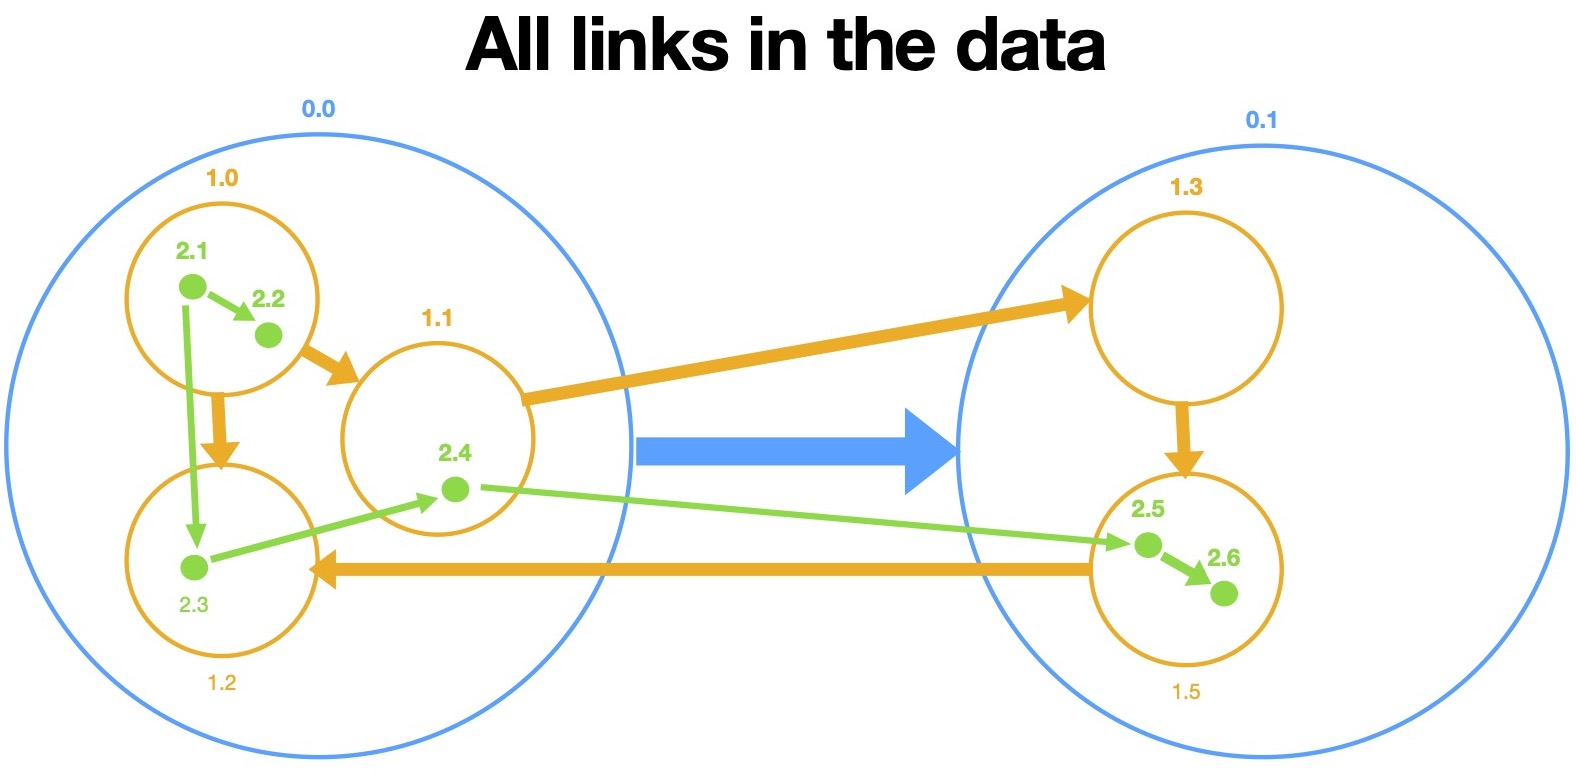
\includegraphics[width=\textwidth, trim={0cm 0cm 0cm 3.5cm},clip]{graphics/filterLinks/allLinks.jpg}
    \caption[A sketch of our layout in 2D.]{A sketch of our layout approach in 2D. Instead of 2D circles, we use 3D spheres in the real application. The size of the nodes is determined by their depth and number of child nodes. The node labels describe their unique ID. This ID consists of two parts: the first number before the dot represents the depth, respectively the layer of the node; the second part is a unique number identifying the node within one layer.} 
    \label{fig:layoutSketch} 
\end{figure}
To achieve \hyperref[req:R1]{R1}, we created a variation of circle packing layout approaches. The core concept is to combine the nested technique of tree maps with multilayer techniques. However instead of flat surfaces as seen in many multilayer network visualizations, we use three-dimensional spheres. 
By using the third dimension, we can achieve a better distribution of nodes and links and therefore display larger networks than with classical 2D approaches, as required in \hyperref[req:R2]{R2}. 
To dynamically build this layout for any given data as input, we developed a custom force based system.
The main goal is to prevent overlapping of nodes while still visualizing the different clusters of hierarchical nodes by proximity. Figure \ref{fig:layoutSketch} shows a sketch of our envisioned layout. The entire data can be seen as a tree structure where each entity in the tree is a graph itself, nested in its parent node. This means that each node can be a super-node or meta-node. Therefore, the number of nodes can grow exponentially with the number of hierarchical layers. Note that the root node is not displayed because it would just create an additional complexity in the visualization without adding any meaningful benefit.

\subsection{Layout Forces and Constraints}
\label{chap:ps-forces}
The force-based layout system consists of multiple forces and constraints to automatically calculate the positions of all nodes. We want to achieve an evenly distributed graph while still fulfilling the requirement rules for hierarchical nesting. Firstly, we define a set of force and constraint templates:
\begin{itemize}
    \item ManyBody-Force: This force is a repulsion force and causes nearby nodes to be pushed away from each other. The strength decreases with the distance of the nodes. This allows the distribution of nodes evenly among the available space.
    \item Link-Force: It is the counterpart of the ManyBody-Force and pulls nodes connected via a link closer together. Together with the ManyBody-Force, it enables us to model a distributed graph while still clustering connected nodes and minimizing the chance for a link to cross a not involved node.
    \item Collision-Force: This force is basically a reinforced version of the ManyBody-Force it prevents nodes from overlapping in the case the ManyBody- and Link-Force push nodes into each other.
    \item Spherical-Constraint: The spherical-constraint is the core concept of our layout we use for nesting nodes. It allows us to “squish” multiple nodes into a sphere for any given point and radius. The center of the sphere can vary for each simulation step. The constraint works by constantly adding a slightly randomized velocity for each node towards the center of the sphere. If the node is outside the sphere, then the velocity is increased drastically.
    \item Center-Force: This force helps us to position the entire visualization in the center of our viewpoint, however there is no strict distance or radius like the Spherical-Constraint applies.
\end{itemize}

It is important to understand that these templates are not applied equally to all nodes. Instead, we apply multiple instances of these forces with different parameters to various subsets of our graph. 
This separation allows us to prevent interference between different groups of nodes for different parents.
Firstly, we distinguish between the top hierarchical layer (from now on called layer $0$) and all other subsequent layers 1,2,3 and so on. Each node and link instance is assigned their respectively layer attribute. Layer $0$ is treated separately because these nodes have no directly assigned parent node. 
For Layer $0$, the center-force with the coordinates $(x:0,y:0,z:0)$, ManyBody-Force, Collision-Force and lastly Link-Force are applied to all nodes and links with a layer $0$ attribute. 
As for layer $1 - n$, we do not apply forces by layer but instead by parent node. For each parent, we add a Collision-Force, ManyBody-Force and Link-Force for all child nodes and links. In addition, the Spherical-Constraint is also added for all child nodes with the position of the parent node as a center. Note that the position of the parent node can change each simulation iteration, so we also update the center position for the Spherical-Constraints.
In conclusion, the total number of forces and constraints in our entire force system (including all layers) is: 
\begin{equation}
    |forces| + |constraints| \: = 4 \, + 4 \cdot |parent\_nodes|
\end{equation}

\subsection{Stability of the force system}

A big challenge for our customized force system was to equally balance all added forces so that each one performs their specific task and does not influence the effect of other forces. To achieve that, we parameterized each force with a strength parameter.
In addition, we also use the concept of an $\alpha$ target from D3-Force \cite{bostock_d3forcejs_nodate}. To put it briefly, it is an additional value, which decreases throughout the simulation. This allows the simulation to “cool down” and stop as soon as it reaches the defined $\alpha$ target value. We use the $\alpha$ target to control the number of simulation iterations. 
Besides balancing the different templates of forces, we also have to decrease the strength recursively for each layer as the nodes and their radius get smaller each layer iteration.
To further improve the stability of the layout, we add a small amount of randomness to the applied velocities and strengths. This improves the node distribution and prevents scenarios where multiple nodes receive the same forces and therefore would overlap each other.
During our optimization, we stumbled upon the problem that nodes tend to jump rapidly to a far position. This happens because we squish the nodes into the sphere of the parent while still applying the ManyBody- and Collision-Forces. Therefore, in some boundary scenarios, the only “free” position for this node is further away which results in the jumping behavior. However, it defeats the concept of successively fine-tuning the positions throughout the simulation steps. For example, nodes of layer 1-3 would be already positioned well but in the last simulation step the parent node in layer 0 would jump and therefore layer 1-3 nodes are positioned outside the parent layer 0 node again. To circumvent that problem, we do not perform the positioning of all nodes throughout the entire simulation. Instead we split up the amount of simulation steps and perform them for each layer successively (see Figure \ref{fig:SimulationSteps}): beginning with positioning the layer 0 nodes, then layer 1 nodes and so on.
Luckily, we also gain a performance benefit through that strategy. 
The reason for this is that, usually the number of nodes grows exponentially for each layer. That means, that a simulation steps for layer5 has to process more individual nodes and forces than a simulation step for layer1. By limiting the simulation steps for the larger growing layers we can reduce the total sum of position update operations.
\begin{figure}[h]
    \centering
    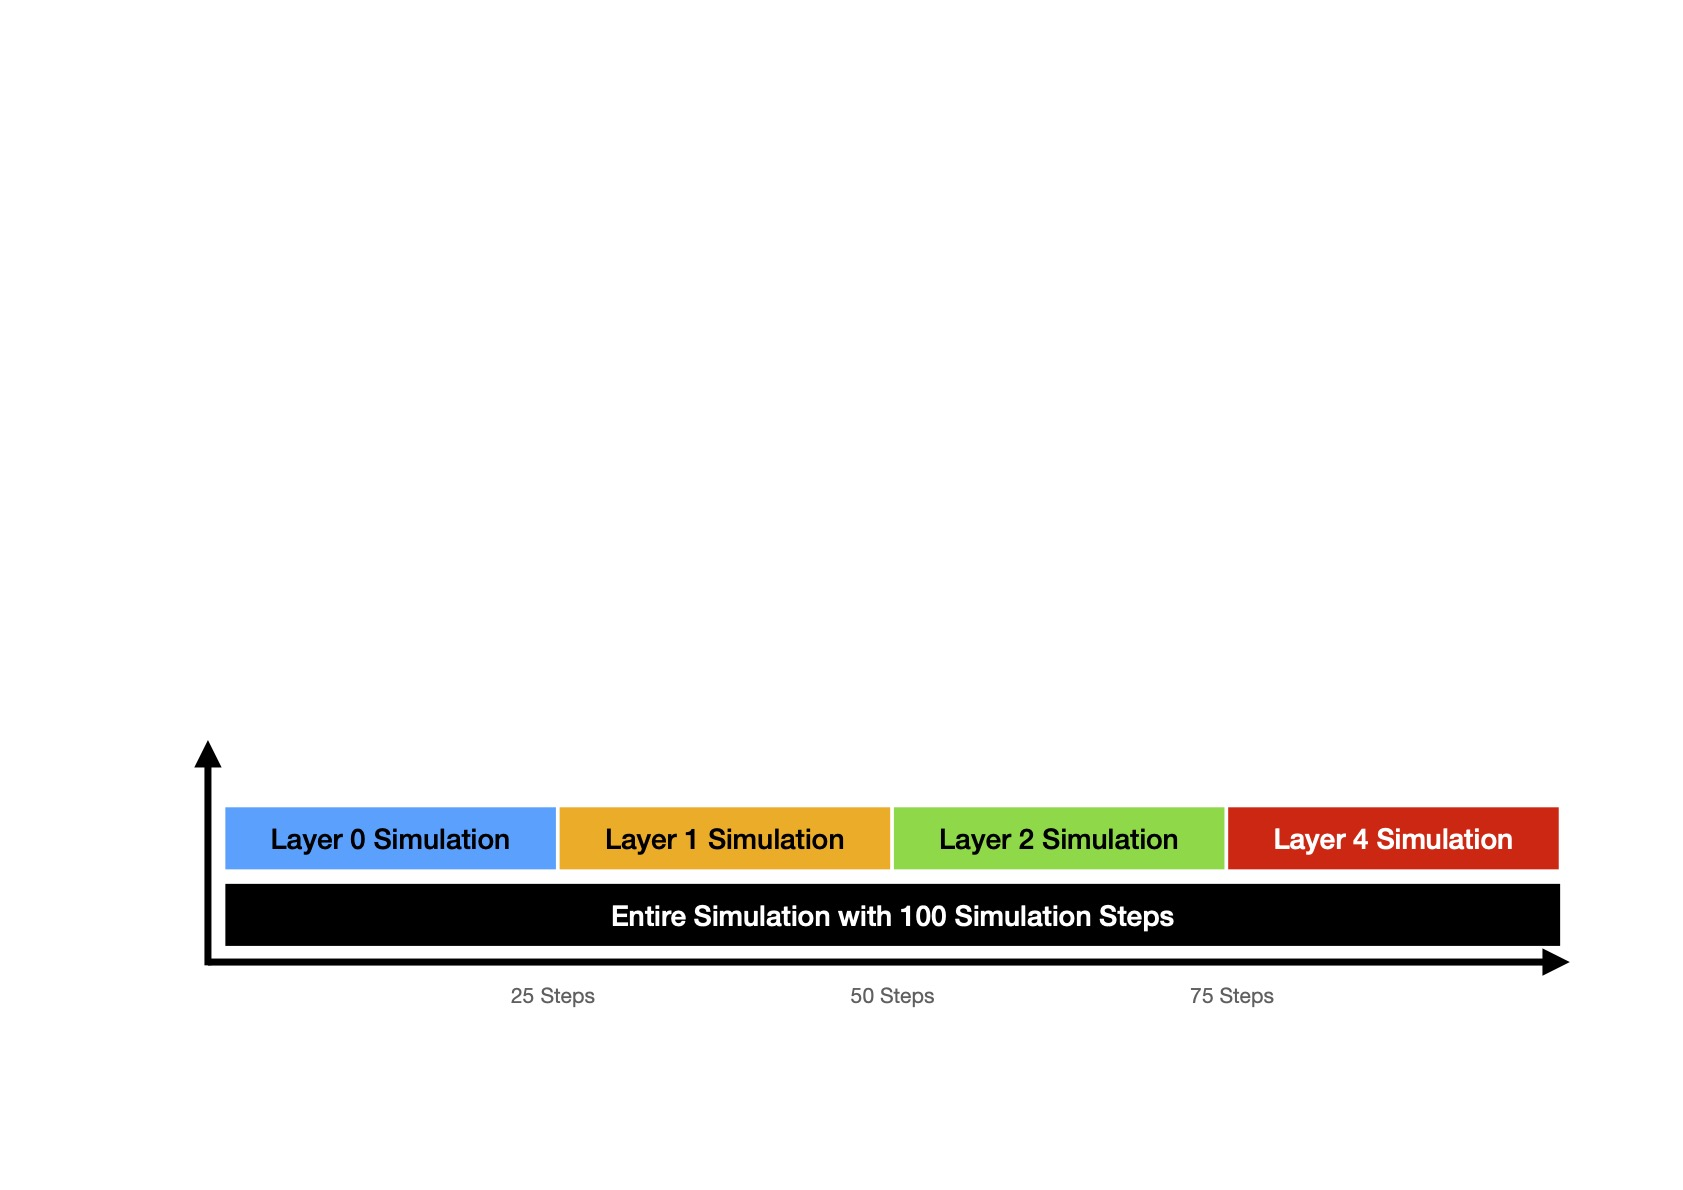
\includegraphics[width=\textwidth]{graphics/simulationStepsSplit.jpg}
    \caption[Distribution of all simulation steps.]{Distribution of all simulation steps for a dataset with 4 hierarchical layers. Each layer receives the same amount of simulation steps, in this case 25 of 100.}
    \label{fig:SimulationSteps} 
  \end{figure}

\section{Graph Visualization}
\label{chap:ps-graphRepresentation}
\begin{figure}[!htb]
    \centering
    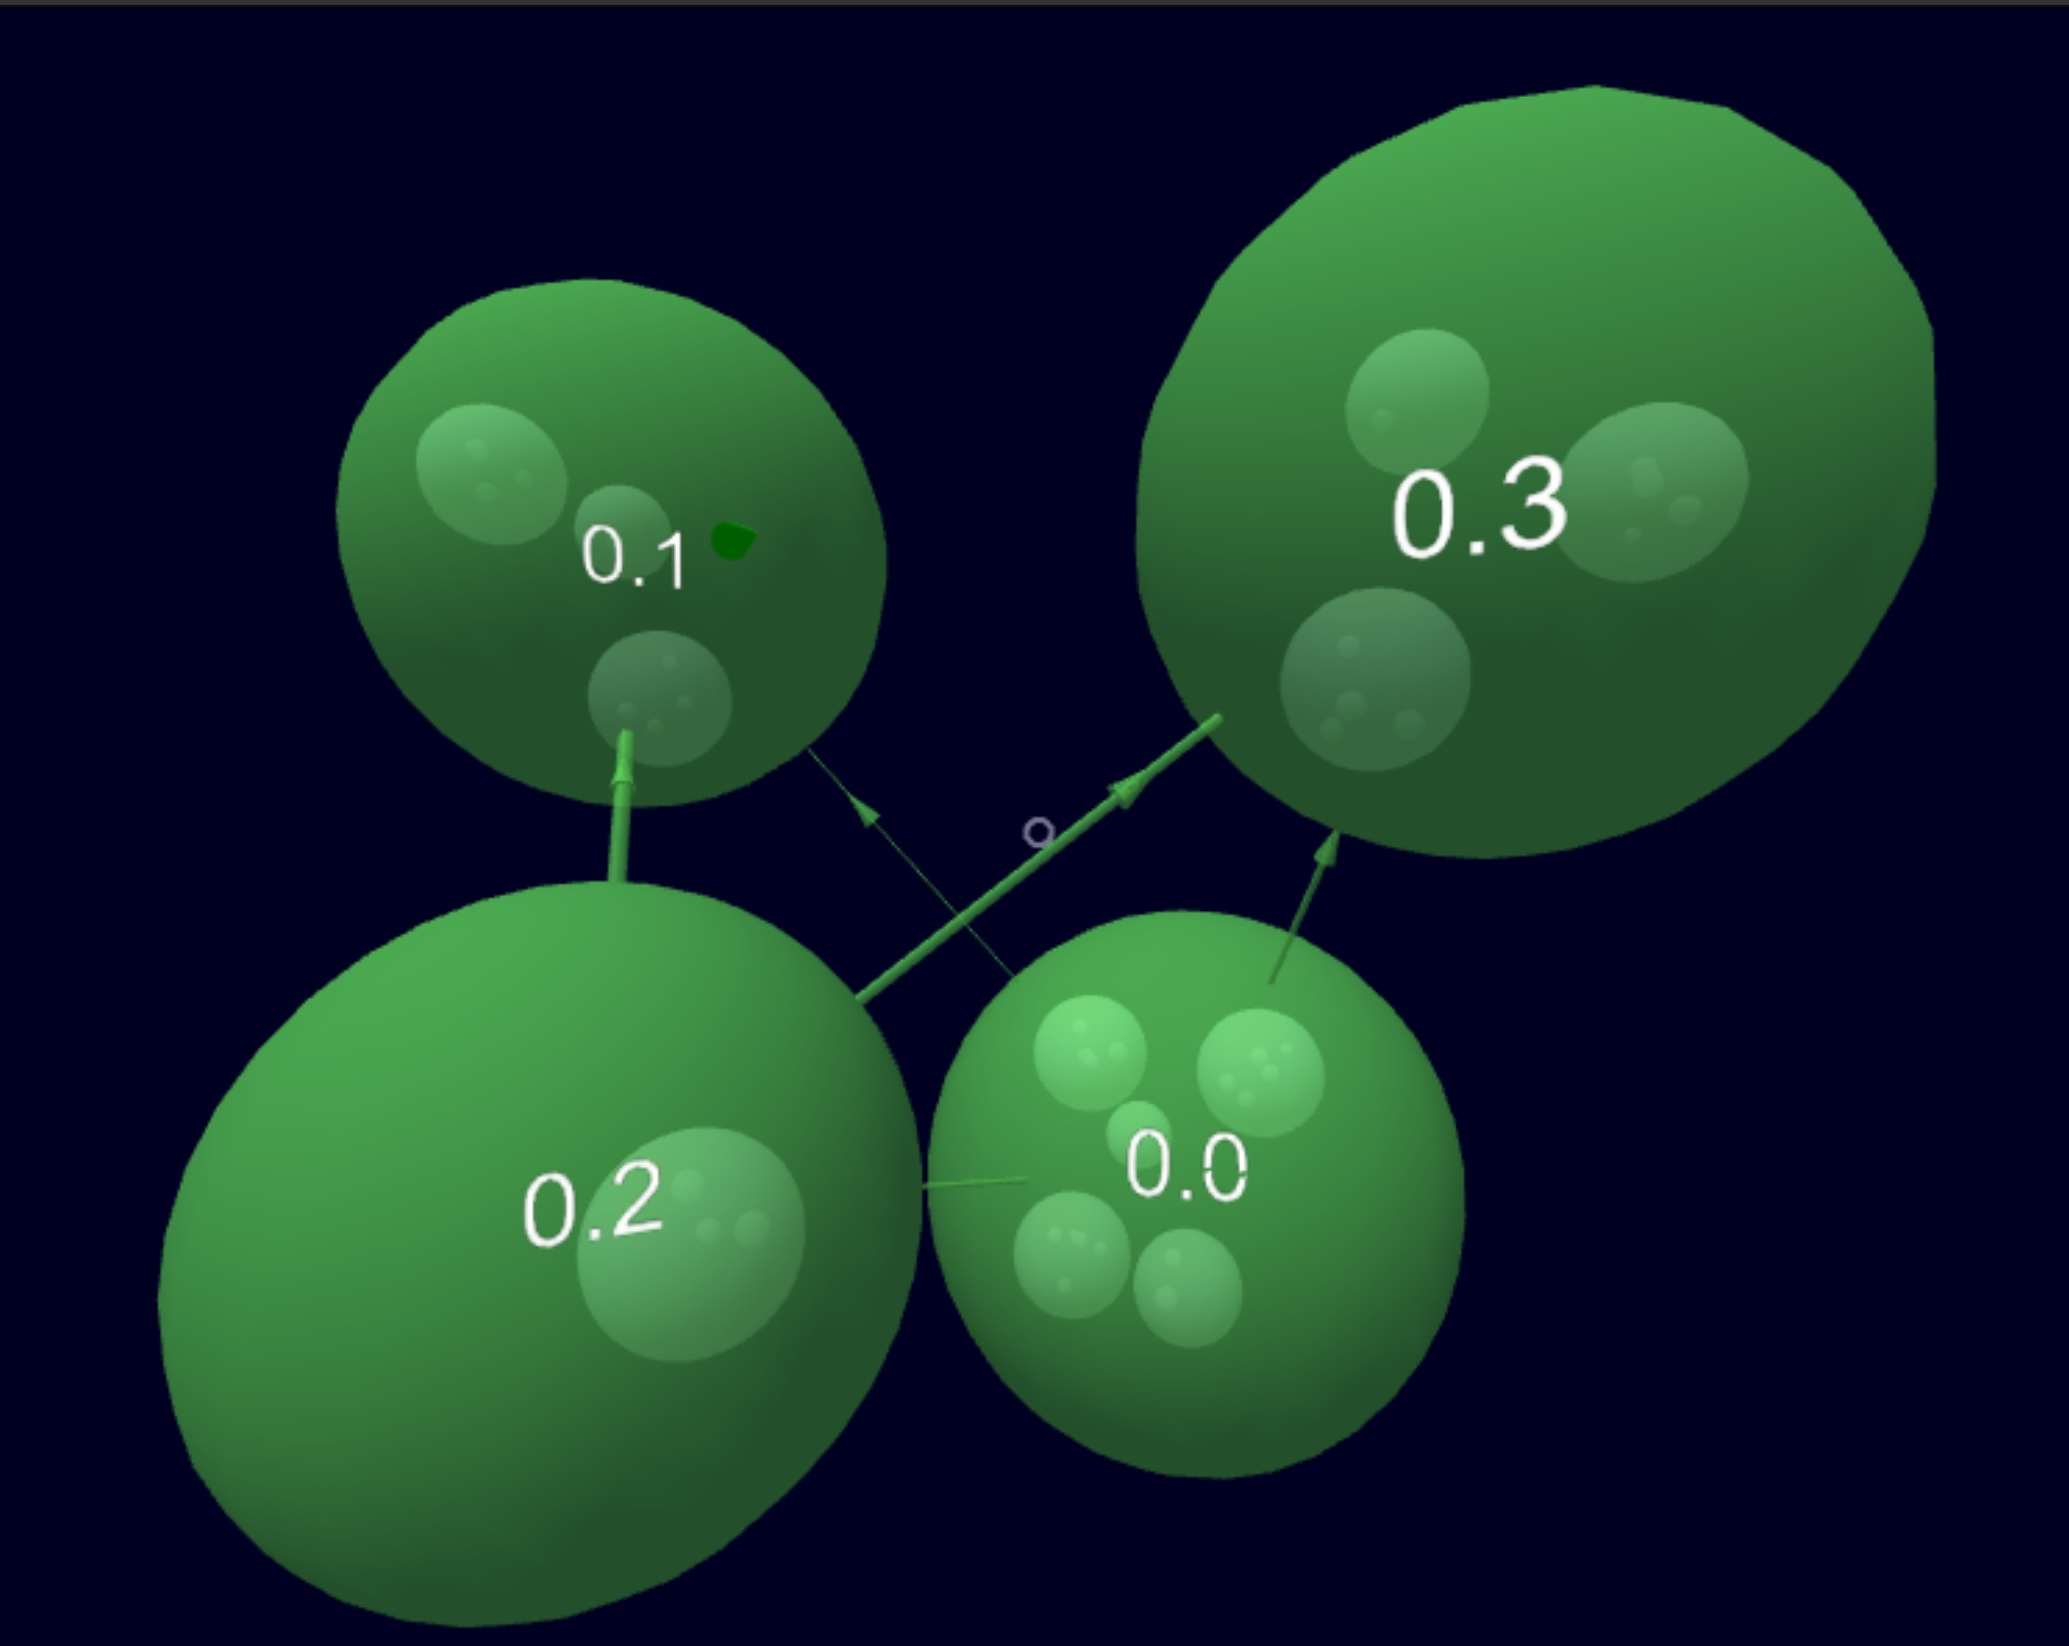
\includegraphics[width=1\textwidth]{graphics/screenshotNesting.jpg}
    \caption[Screenshot of the visualization.]{Overview perspective of the visualization: Each node is rendered semi-transparently. This allows the user to detect the overall topology of the data.}
    \label{fig:ps_nestedLayout}
\end{figure}
\begin{figure}[!htb]
    \centering
    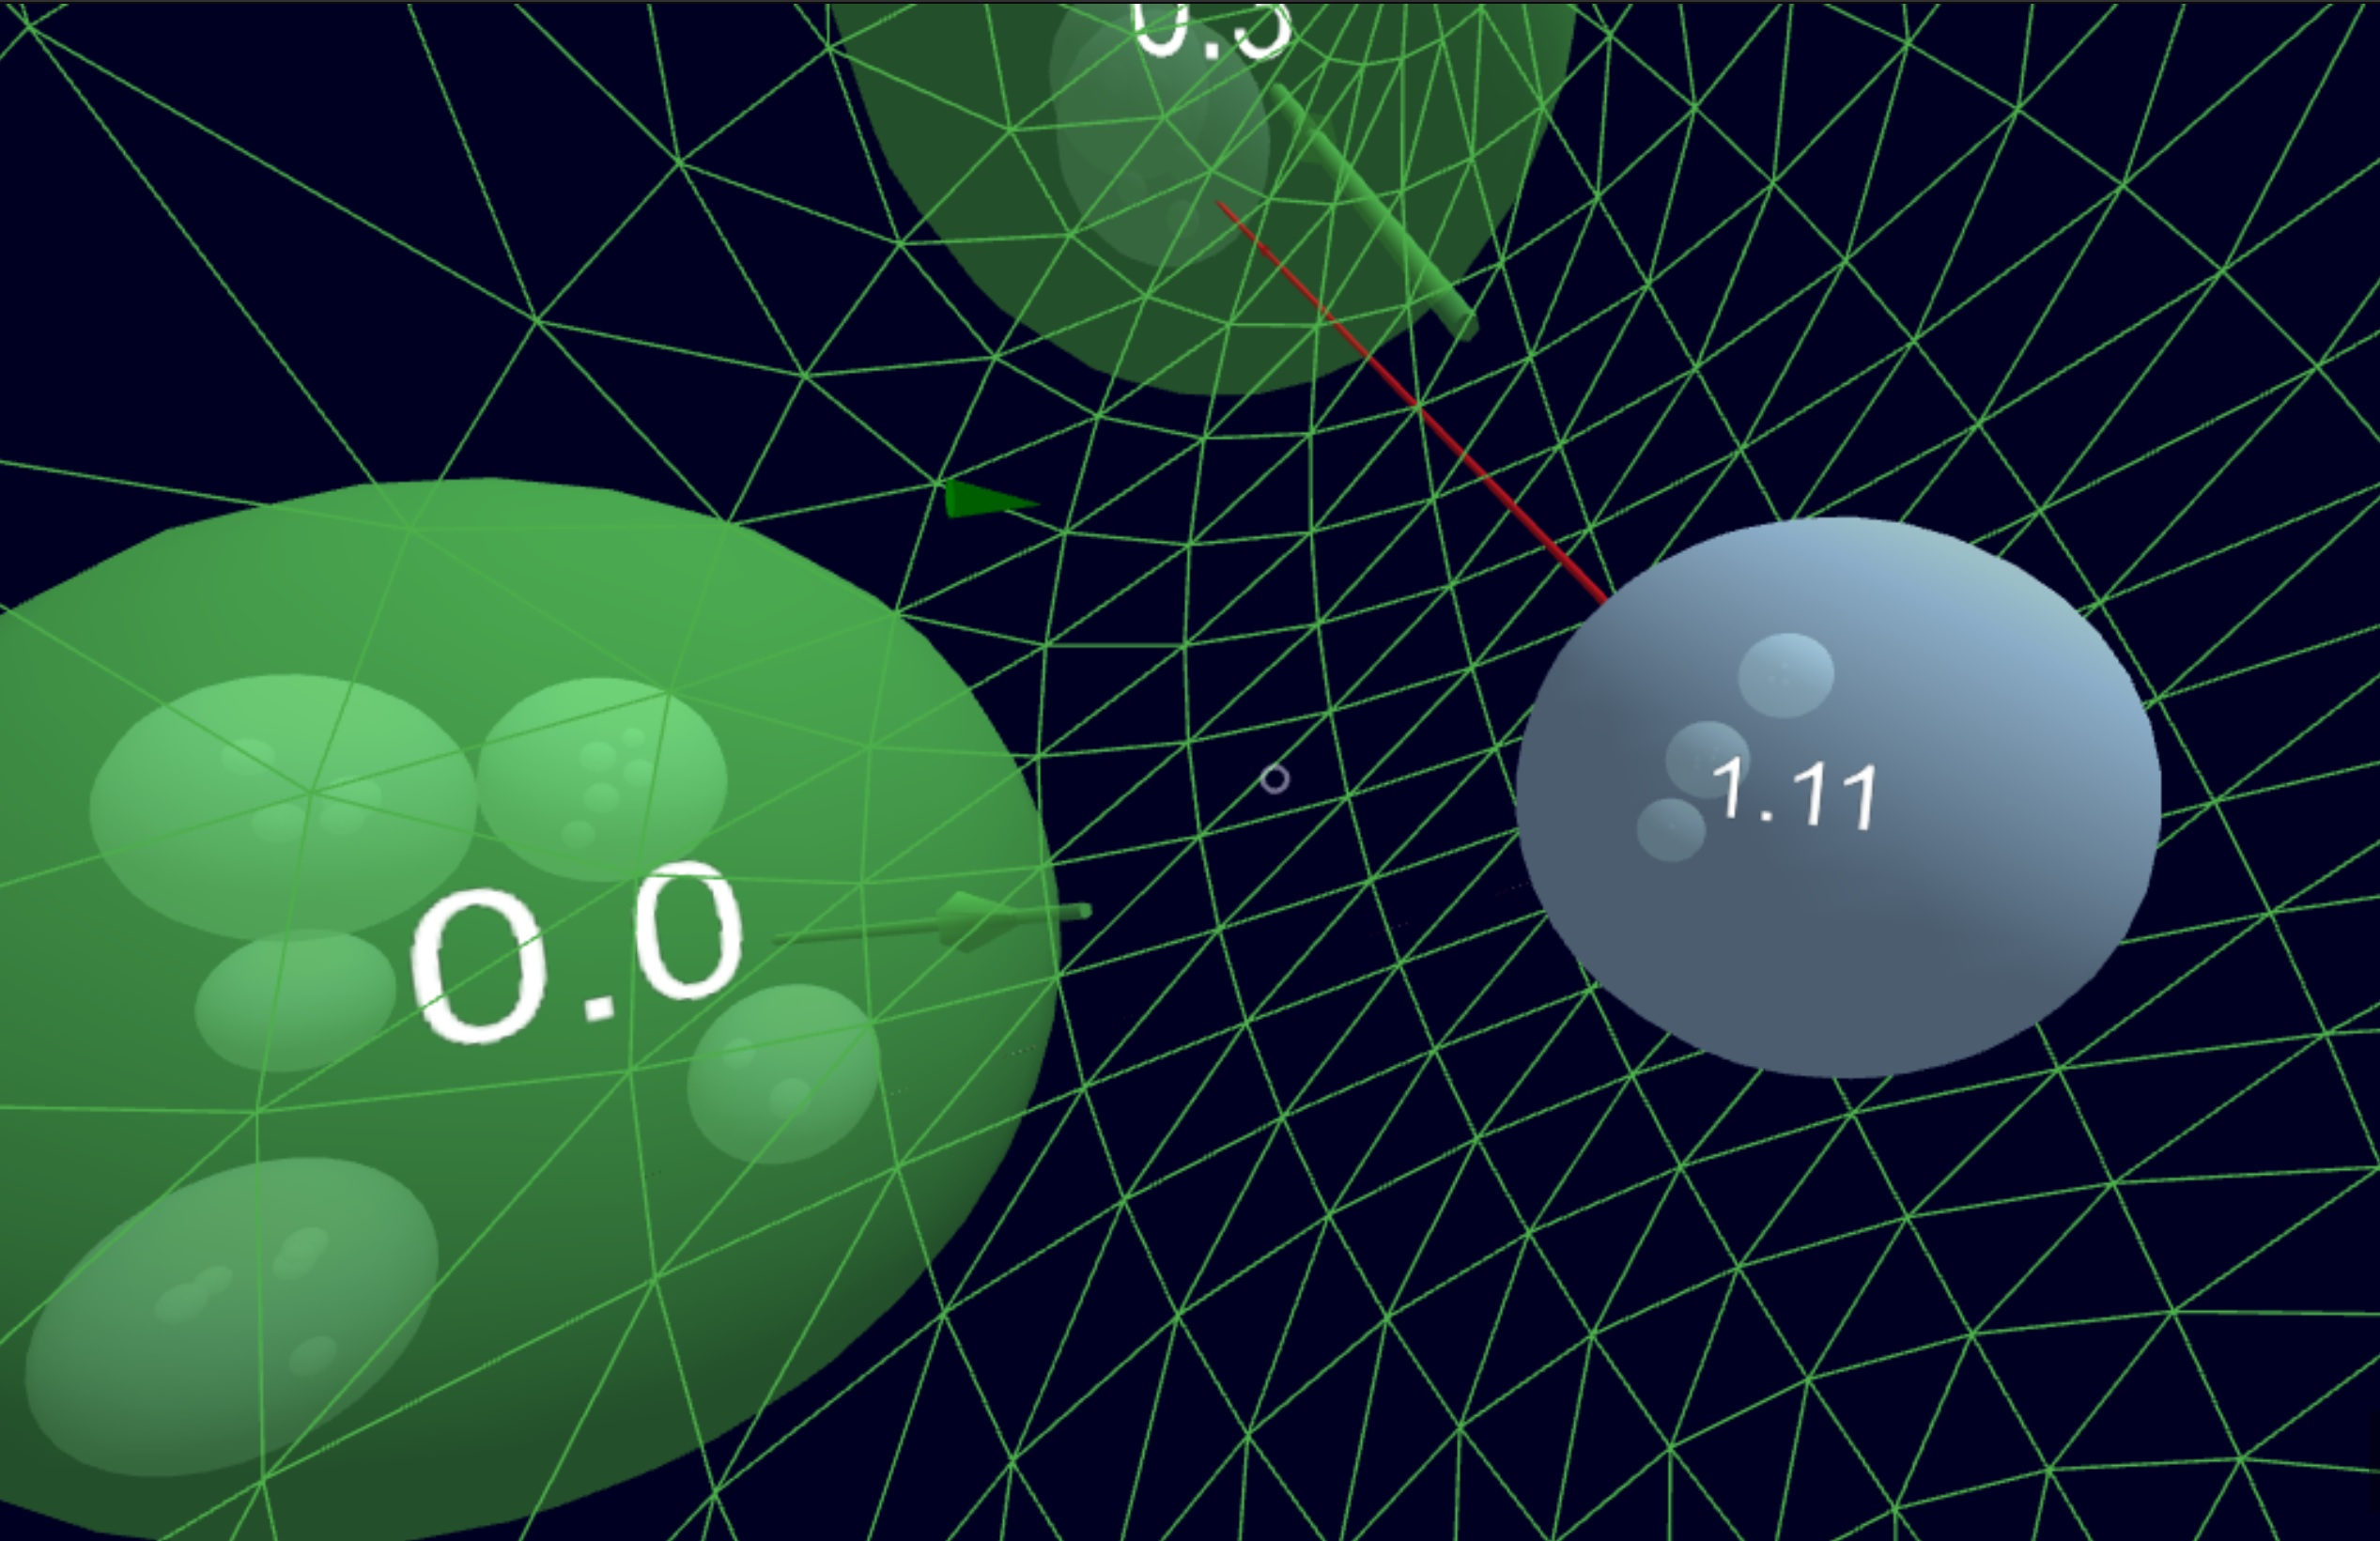
\includegraphics[width=1\textwidth]{graphics/screenshotNestingAndWireframe.jpg}
    \caption[Screenshot of the visualization.]{Detail perspective inside of node 0.2: To be able to tell the border of the nodes, the node is rendered as a wireframe when looking from the inside out.}
    \label{fig:ps_wireframe}
\end{figure}
The goal of the graph visualization was to choose appropriate visual encoding which allow us to reduce visual clutter and improve clarity while still displaying as much data as possible.
To represent the graph, we choose spheres for nodes, tubes as links and cones as arrow heads indicating the link direction.
With solid textures, the overview ability of the visualization would be poor since our layout approach uses nested layers. Therefore, the user could only see one layer of nodes at the same time. To circumvent that we render all nodes transparently. Then, the user is able to see the nested nodes inside their parent node (see Figure \ref{fig:ps_nestedLayout}). 
However, links inside other nodes are not visible because displaying many links would increase visual clutter and reduce overview. To deal with the large amount of links, we apply filter conditions, which are described in Section \ref{chap:ps-filterLinks}.
When the user is inside a node, the transparent sphere of the node is not rendered anymore. Instead of a solid transparent sphere, we render a wireframe (see Figure \ref{fig:ps_wireframe}). The improved spatial impression given by the virtual reality experience allows the user to better see the boundary of the wireframe than visible in the Figure. To further improve the assignability of nodes to their layers, each node and link of the same layer shares a predefined color.
For each node instance, a billboard text label is placed on the border of the node and always points towards the camera. For our artificially dataset the ID of the node is displayed, for a real dataset it would display the appropriated node and cluster names.

Our adapted sphere packing layout algorithm requires us to render nodes and links smaller for each nested sphere. To achieve that, we added a dynamically scaling factor that is applied for each rendered entity (node, link, text-label). 
In addition to the rendering algorithm, the force algorithms also uses that scaling factor to ensure a correct collision detection and sphere packing. 
This globally scaling factor is described by the following formula: 
\begin{equation}
    s_{ d } = \frac{1}{(d+1)^{(d+1)} \cdot s}
\end{equation}
Where $s_{ d }$ is the resulting scaling factor, $d$ is the depth of the current layer and $s$ is a global constant that allows us to balance the force algorithm according to the rendering objects. The resulting scaling factor is used, in combination with the number of child nodes, to calculate the size of the node: 
\begin{equation}
    r_{ d,i } = (r \cdot s_{ d }) + (\left\lvert N_{ d,i } \right\rvert \cdot rs)
\end{equation}
Where $d$ is the depth, i the node index at depth $d$, r is a base radius, $s_{ d }$ is the previous scaling factor, $\left\lvert N_{ d,i } \right\rvert$ is the set of child nodes of the node $i$ at depth $d$, and $rs$ is a global constant to balance the size of the node radius to the according force radius.

\section{Interaction}
\label{chap:solution-interaction}

\begin{figure}[b]
    \centering
    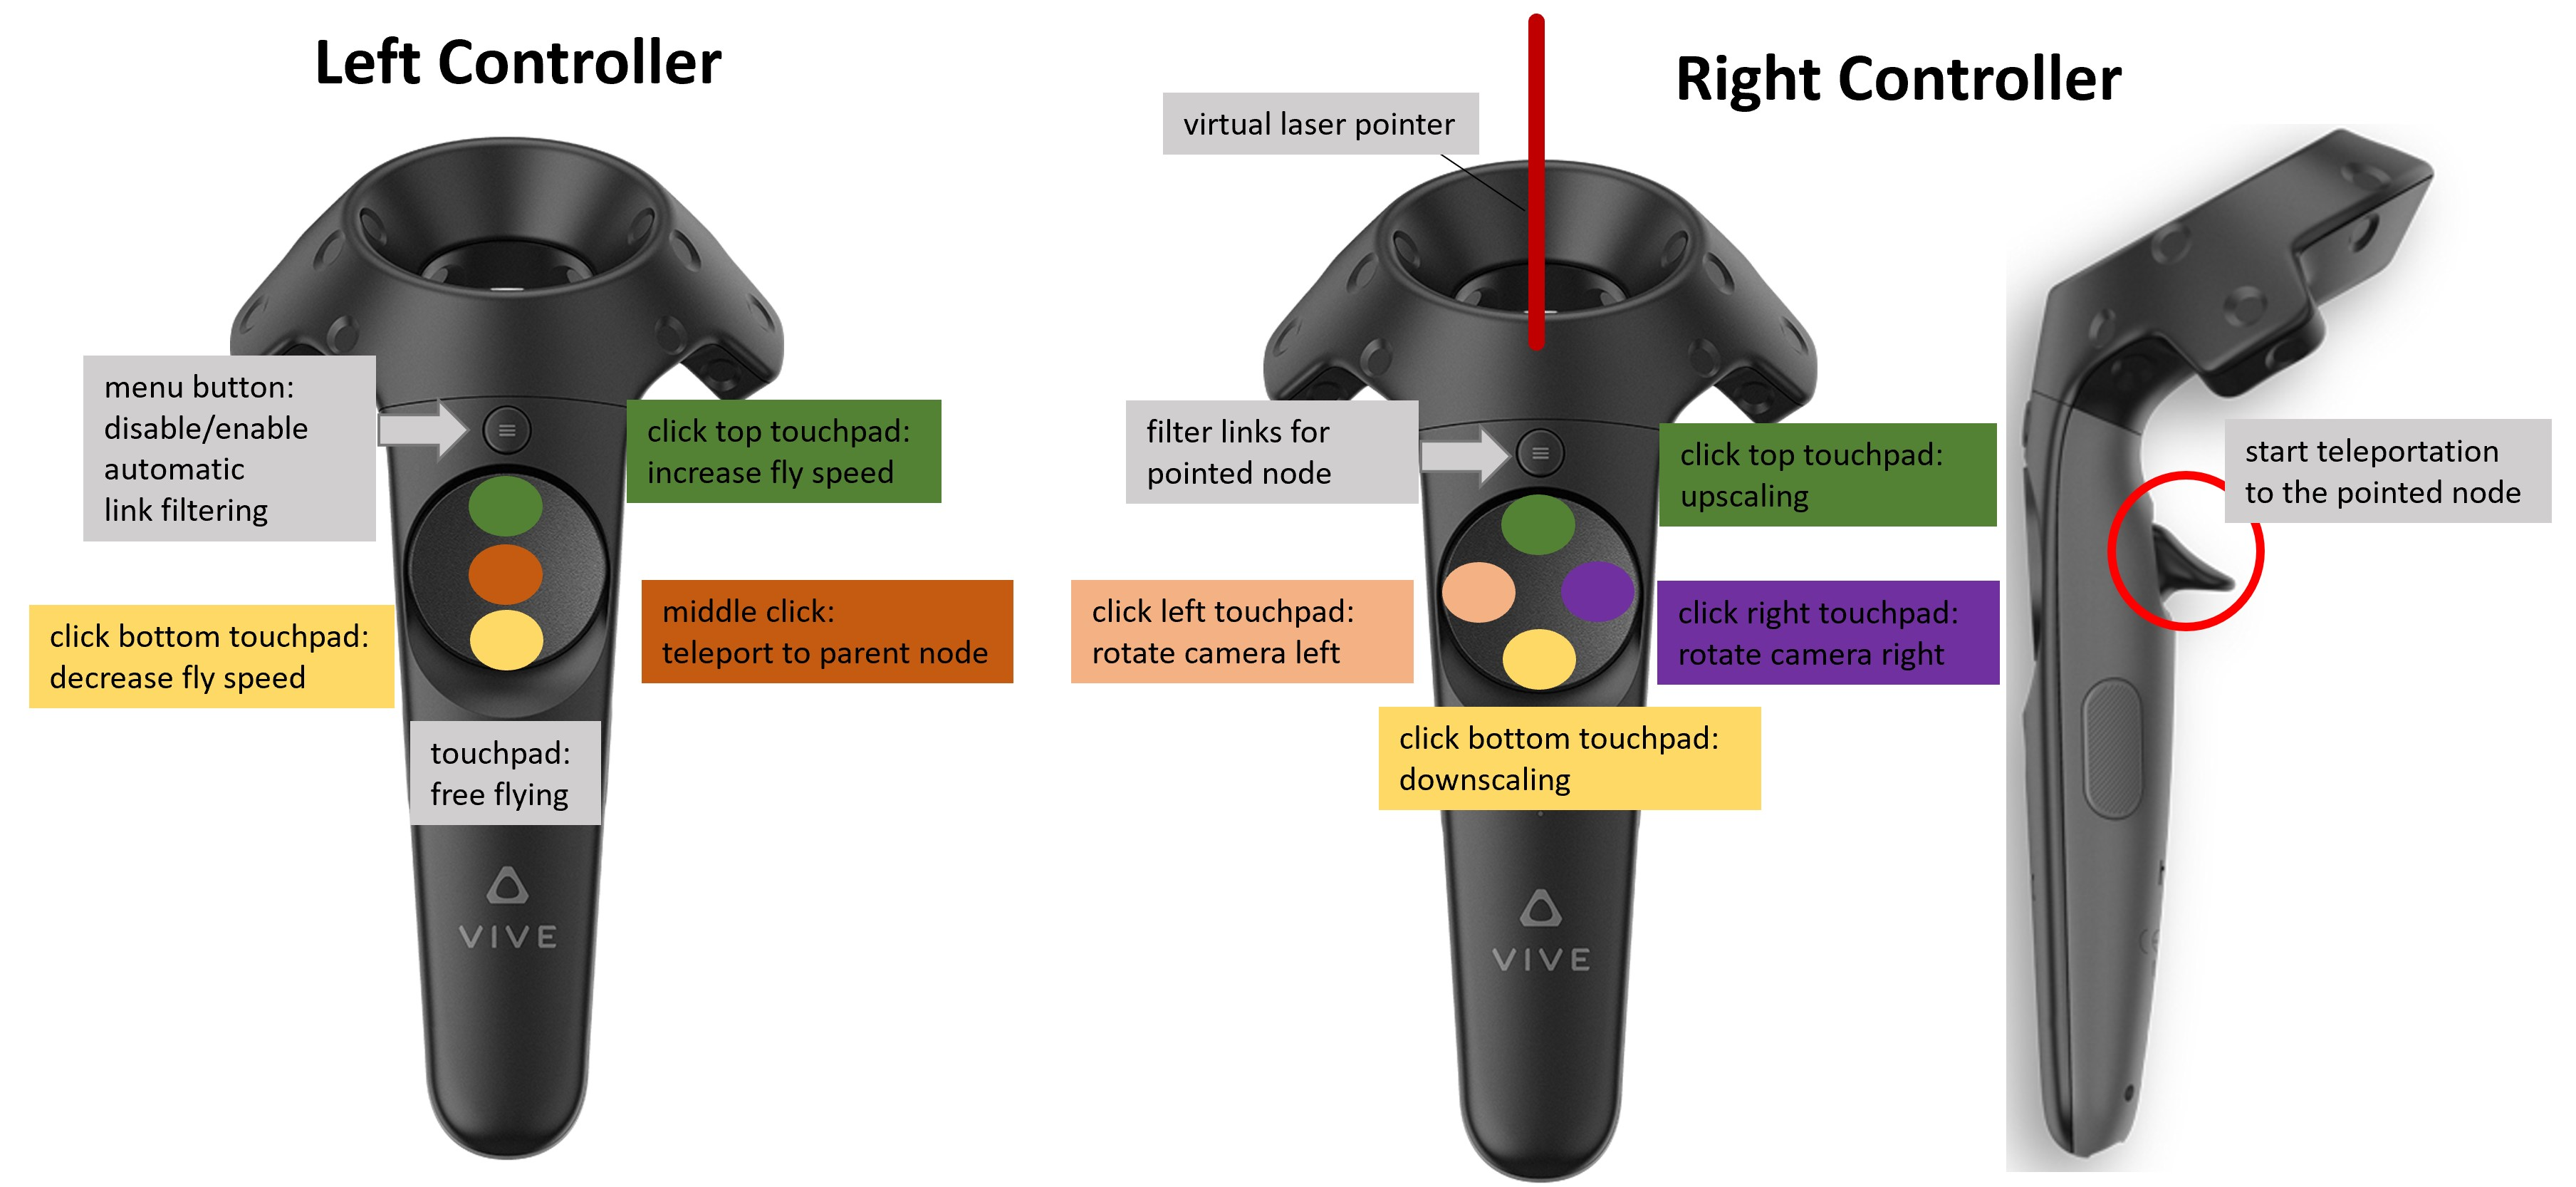
\includegraphics[width=1\textwidth]{graphics/controllerMapping.jpg}
    \caption[Our controller mapping for the interactive VR experience.]{Our controller mapping for the interactive VR experience. Depending on the clicking position on the touchpad, different actions can be called. The different clicking positions are marked in the image with different colors.} 
    \label{fig:controllerMapping} 
\end{figure}
For achieving \hyperref[req:R4]{R4}, we use the 6 DOF tracking of the headset and controllers from the HTC Vive. Therefore, we aimed to implement intuitive interaction techniques to allow teleportation navigation throughout the virtual scene (see Section \ref{chap:solution-navigation}). In addition, the user should be able  to switch the visibility filter between multiple groups of links (see Section \ref{chap:ps-filterLinks}).
What both interactions have in common is that the user has to select a specific node before these actions can be triggered. 
This concludes that our visualization needs a general way to support the selection of nodes which then can be used by various other methods we apply during the exploration process. 
In addition, we also stated in our requirements that we strive to use the tracking capabilities of VR to create intuitive interaction methods.
Therefore, all user interactions can only be provided by the native VR supported hardware, in particular from 6-DOF tracked controllers. 
To this end, we use the common concept of ray cast selection for selecting nodes in the virtual scene. Along the length of the right controller, a ray is cast through the scene. 
To better visualize the effect, we render a straight red line to imitate a virtual laser pointer (see Figure \ref{fig:screenshot_interaction}). 
The first intersected node is then used as the selected node for other methods like filtering or teleportation. The node label of the selected node is displayed in a Head-up-Display element centered in the lower part of the screen inside the headset (see Figure \ref{fig:screenshot_interaction}). 
In addition, the selected node and directly connected nodes are visually highlighted (see Figure \ref{fig:screenshot_interaction}). This allows the users to quickly see, which node they currently have selected and provides the context of the connected nodes.

\begin{figure}[h]
    \centering
    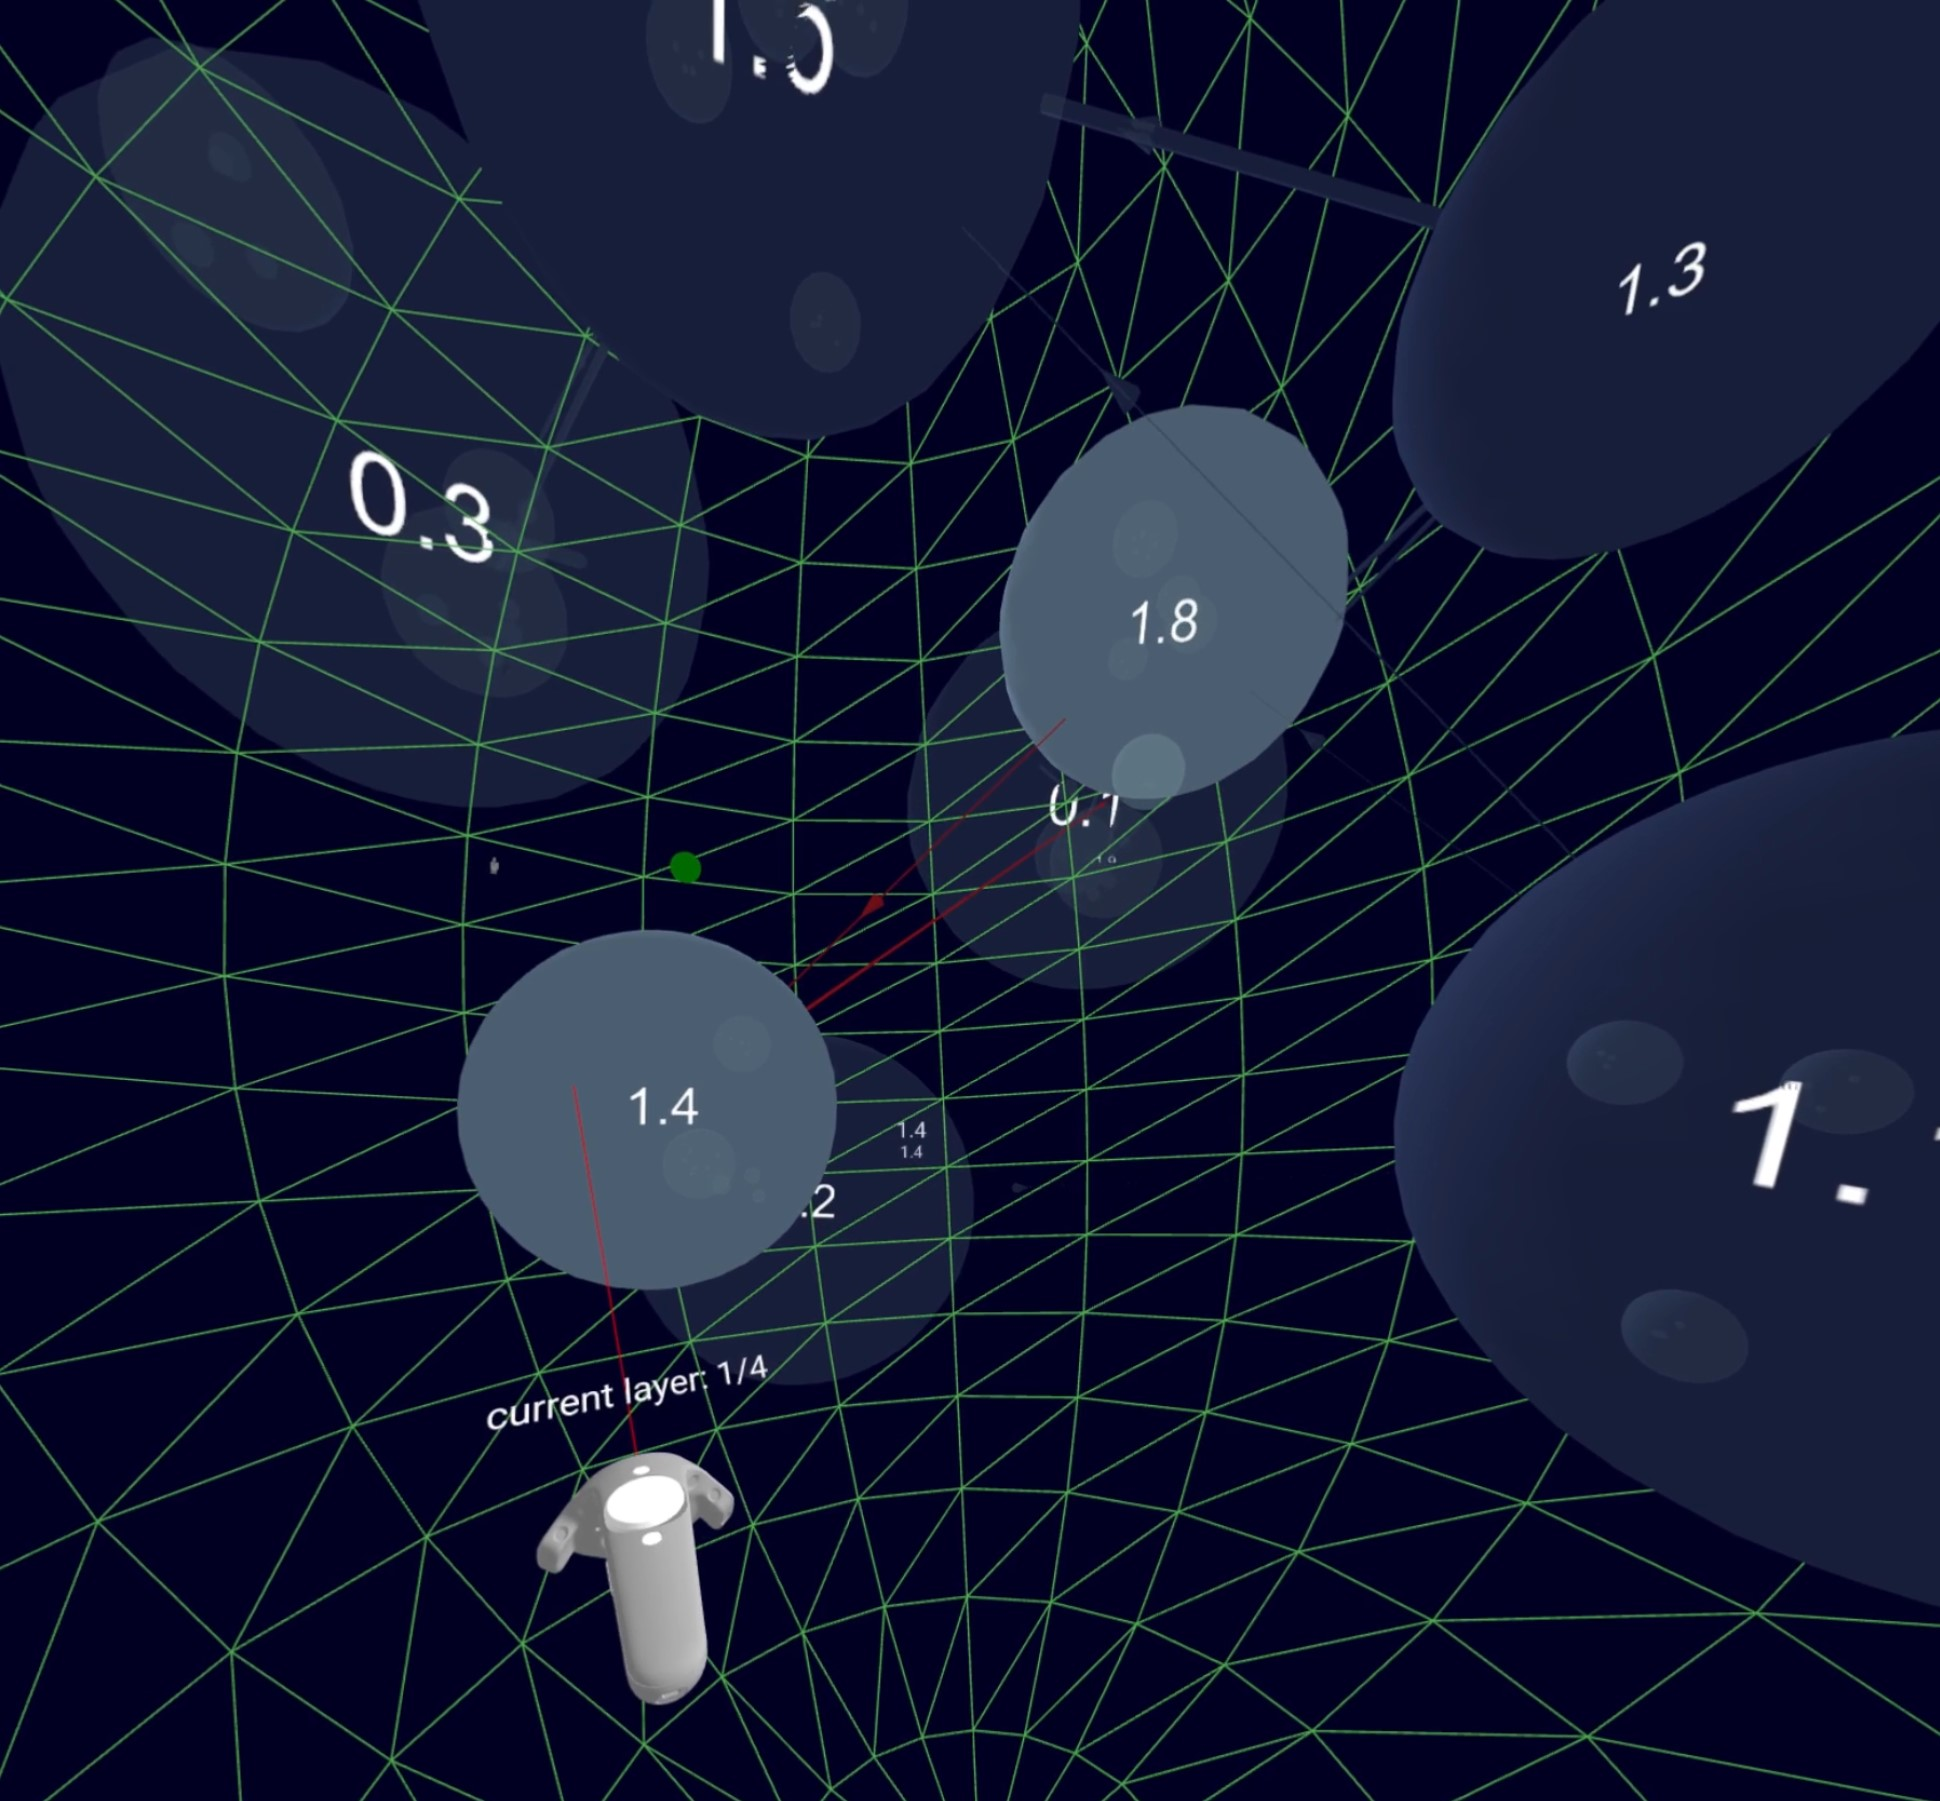
\includegraphics[width=1\textwidth]{graphics/screenShotFilteringNodes2.jpg}
    \caption[Screenshot during the selection of a node.]{Screenshot during the selection of a node: The user can see the virtual laser pointer as a red line. 
    In the lower part of the screen, the node label (1.4) of the pointed node is written (in this screenshot it is centered in the middle of the screenshot, because the field of view in the headset is different as in the screenshot).
    In addition, the selected node, as well as directly connected nodes, are highlighted in a brighter shading. For improved navigation, the layer where the user currently is located in is displayed as a text above the controller.} 
    \label{fig:screenshot_interaction} 
\end{figure}

Now that the users can select specific nodes in the scene, we also have to give them the opportunity to trigger certain actions. These actions include the teleportation navigation (see Section \ref{chap:solution-navigation}) and the link visibility filter (see Section \ref{chap:ps-filterLinks}). 
Other actions do not require the selection of a node, i.e., manual rotation, free flying with an adjustable flying speed, and teleportation to an upper layer (see Section \ref{chap:solution-navigation}), as well as manual scaling (see Section \ref{chap:ps-spatialReference}).\\
However, we have to assign each of these actions to a button on the controller (see Figure \ref{fig:controllerMapping}). In order to provide a smooth workflow, we extend the normal trackpad click by the position of clicking. 
This allows us to have 5 virtual buttons on the trackpad: top, bottom, left, right and center. The advantage of this method is that these virtual buttons can be used fluently while also interacting with the touch sensitive trackpad at the same time by one finger. 
Therefore, the users can control the free flying direction and speed with their left thumb, as well as triggering the teleportation to the upper hierarchical layer. The right controller acts as a virtual laser pointer. The two actions, which need a node selection beforehand, can be started by the menu button and trigger. 
On the right trackpad, the scaling and rotation can be controlled.

We optimized our application for the HTC Vive. Therefore, all described button mappings refer to the HTC Vive controllers. However, we only use simple buttons, trackpads and industry standard tracking methods. 
As other 6-DOF headsets usually provide the same or similar interaction possibilities, the interaction concept of our visualization can be applied to other headsets as well.

\subsection{Filtering Link Visibility}
\label{chap:ps-filterLinks}

\begin{figure}[p]
    \centering
    \begin{subfigure}{0.6\columnwidth}
        \centering
        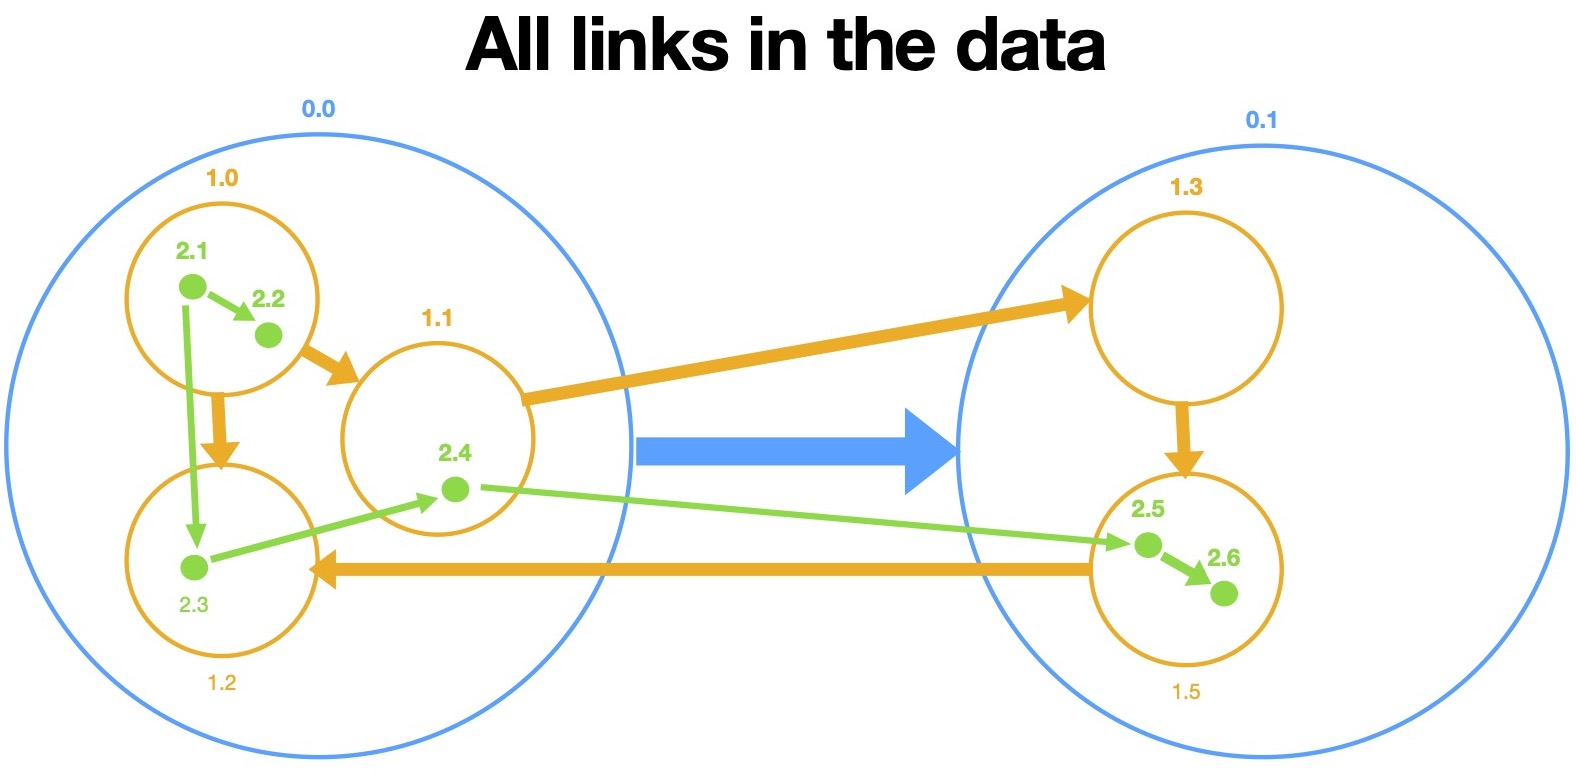
\includegraphics[width=\textwidth]{graphics/filterLinks/allLinks.jpg}
        \subcaption{All links represented in the data.}
        \label{fig:linkFilter-all}
    \end{subfigure}
    \begin{subfigure}{0.6\columnwidth}
        \centering
        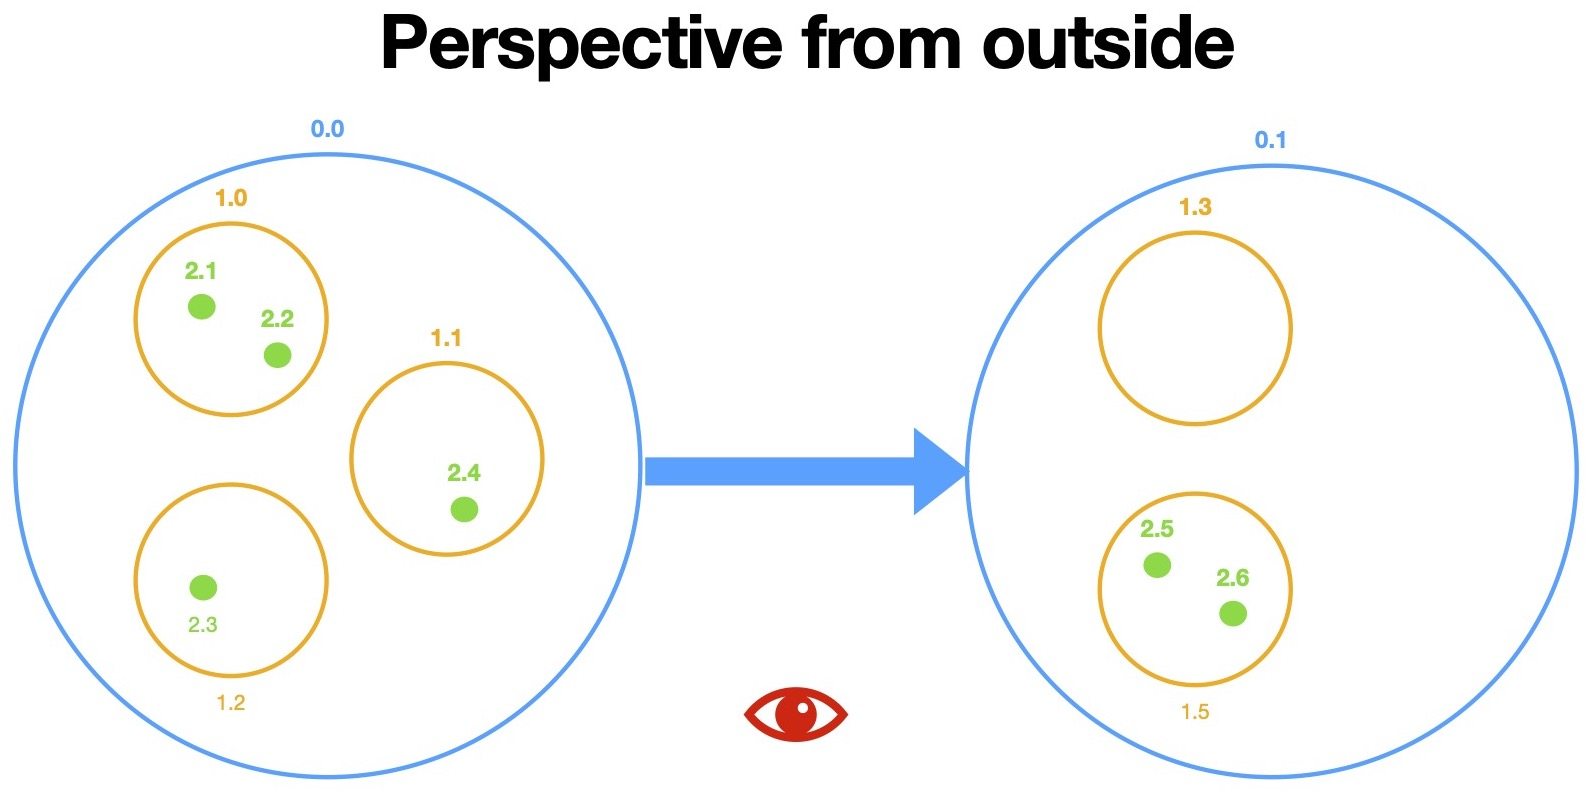
\includegraphics[width=\textwidth]{graphics/filterLinks/outside.jpg}
        \subcaption{Visible links when the user is outside every node.}
        \label{fig:linkFilter-outside}
    \end{subfigure}
    \begin{subfigure}{0.6\columnwidth}
        \centering
        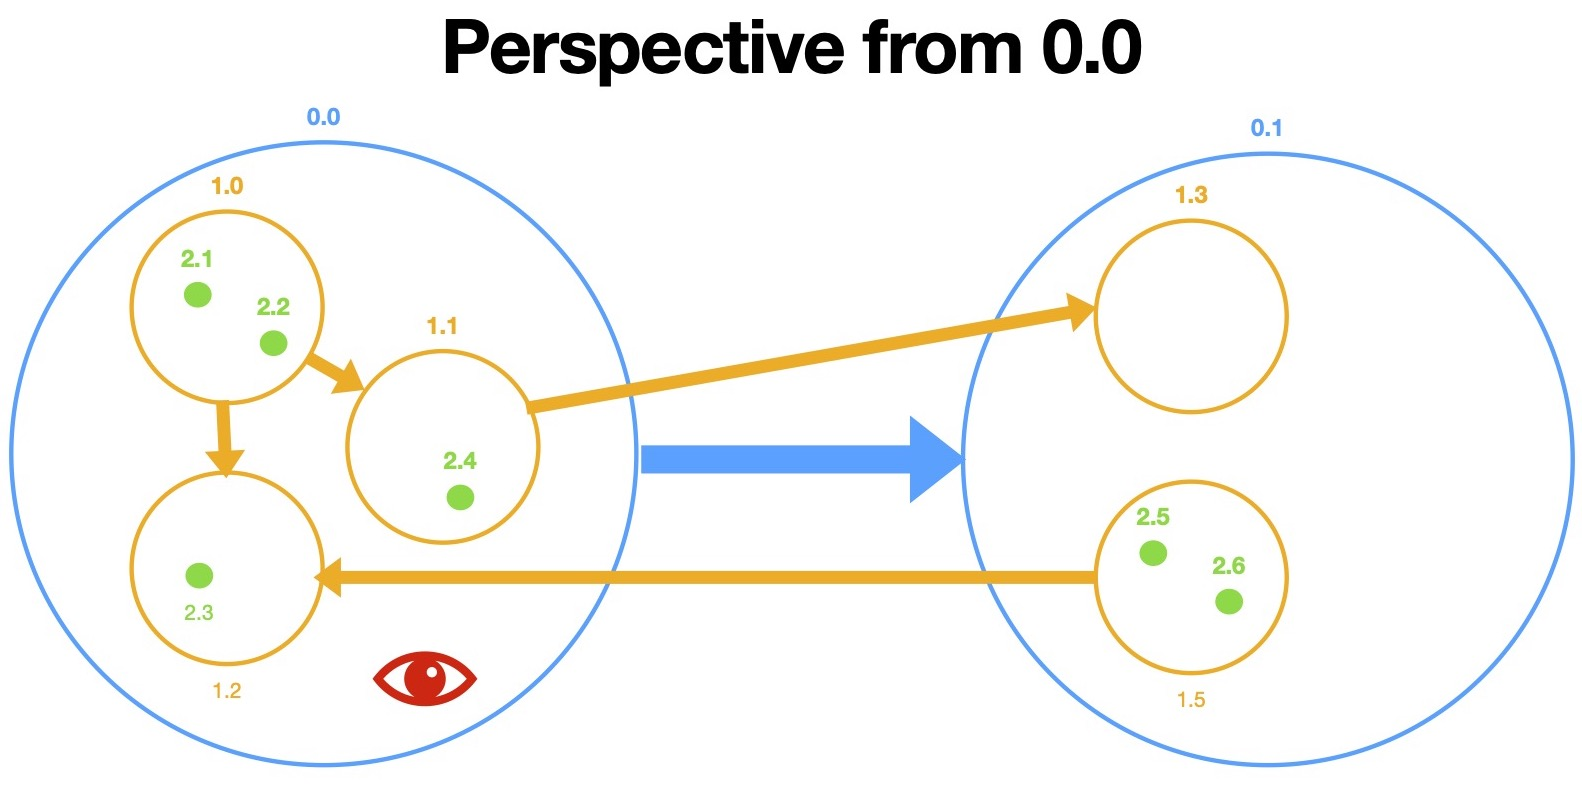
\includegraphics[width=\textwidth]{graphics/filterLinks/layer0.jpg}
        \subcaption{Visible links when the user is inside node 0.0 or when node 0.0 is selected by the laser pointer interaction.}
        \label{fig:linkFilter-layer1}
    \end{subfigure}
    \begin{subfigure}{0.6\columnwidth}
        \centering
        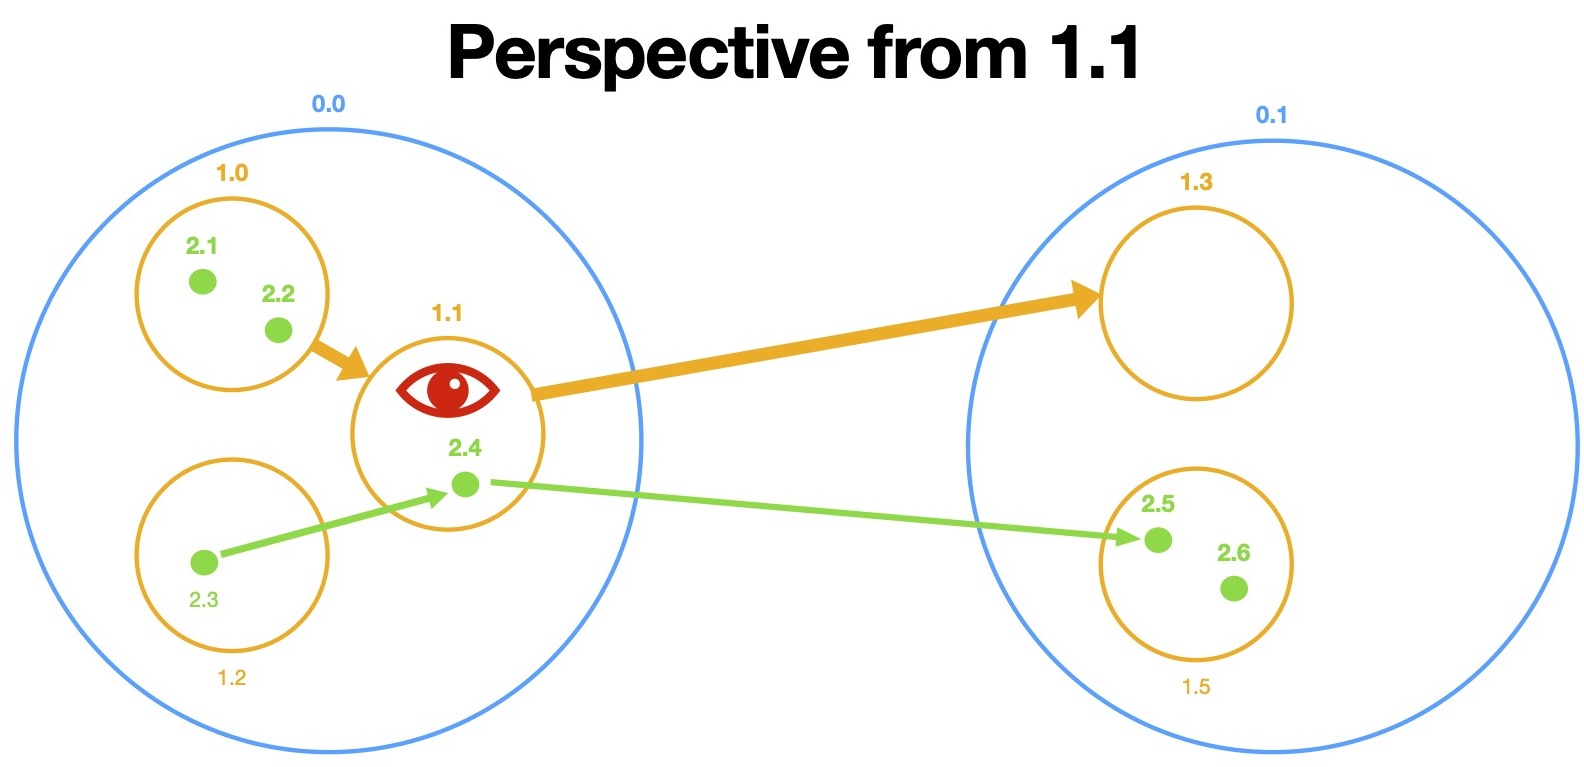
\includegraphics[width=\textwidth]{graphics/filterLinks/layer1.jpg}
        \subcaption{Visible links when the user is inside node 1.1 or when node 1.1 is selected it by the laser pointer interaction.}
        \label{fig:linkFilter-layer2}
    \end{subfigure}
    \caption{Our filtering technique visualized on a small example graph.} % Remove the [...] argument if the original caption should be used in the figure list.
  \end{figure}

To ensure the clarity of the visualization (see \hyperref[req:R6]{R6}) and display larger networks than 2D approaches (see \hyperref[req:R2]{R2}), we apply a filtering approach for links according to the requirements. 
The goal is to reduce visual clutter while providing as much information as possible. 
As a quick recap: Links in our visualization can exist between nodes within the same hierarchical parent node but also to nodes with a different parent node as long as the hierarchical depth is the same. Figure \ref{fig:linkFilter-all} shows a small example of all possible link combinations for three hierarchical layers.
Displaying all links at the same time would quickly lead to visual clutter where a meaningful exploration is not possible anymore. 
Therefore, we came up with our own filtering logic that decides which links are displayed and which are not. 
The filter uses a specific node. This can either be a directly selected node from the user (by the laser pointer interaction) or an indirectly selected node through the position of the user. A directly selected node always overrules the indirectly selected one. Our filter logic uses the following rules:

\begin{enumerate}
    \item If no node is selected and the user is not inside any node only the links from the top layer 0 are displayed (see Figure \ref{fig:linkFilter-outside}).
    \item All directly connected links to the selected node are displayed (currently our visualization only supports links between nodes with the same depth $d$).
    \item All links connected to direct child nodes from the selected node are displayed. Direct child means the depth of the child node is $d+1$. 
    \item All other links are not visible.
\end{enumerate}

As an example, Figure \ref{fig:linkFilter-layer1} shows a situation where node 0.0 is selected. Therefore, all links connecting direct neighbor-nodes of 0.0 and links to the child-nodes of 0.0 itself are displayed. However, links of deeper nested nodes, like 2.1, are not displayed. 
A different situation can be seen in Figure \ref{fig:linkFilter-layer2}: here only links from node 1.1 and 2.4 are visible but the links from node 1.2 and 0.0 are not visible anymore.
In an earlier version, we not only displayed the links of direct child nodes but instead links of all recursive child nodes. For example, in Figure \ref{fig:linkFilter-layer1}, the green links would also be visible. However, this quickly leads to visual clutter. Therefore, we kept the direct child approach.

In order to support an intuitive and flexible exploration workflow, the user also has the ability to lock a currently applied filter.
With the left menu button (see Figure \ref{fig:controllerMapping}), the state of the lock can be toggled. 
If the lock is active, the indirect selection of nodes by the position of the user is disabled. The lock is also automatically set active if a node is manually selected by the laser pointer. 
This allows the user to freely navigate around the visualization without constantly having to deal with changing link visibility. 
On freeing the lock, the indirect selection of nodes automatically kicks in again and selects the current node the user is positioned in.

\section{Navigation}
\label{chap:solution-navigation}
In order to fulfill \hyperref[req:R3]{R3}, we support a walkable room scale VR experience setup to navigate the virtual scene. As we stated in Section \ref{chap:rw-vrnavigation}, walking probably provides the best immersive and intuitive navigation method.
However, the graph will usually be larger than the user's available space. To this end, we also include other navigation methods.
To allow maximum of flexibility during the navigation, as required for \hyperref[req:R5]{R5}, we provide two navigation methods: animated teleporting for covering larger distances and free flying to perform small and precise position adjustments.

The user should be able to move to other distant parts of the graph without loosing orientation or being interrupted in the exploration flow. A common example is to jump to a connected node of another parent node. 
Therefore, we implemented an animated teleportation method. The user can select a node with the laser pointer and then press the right trigger to initiate the teleportation. The target position is the closest edge barely inside the node. This allows the user to get an overview of all nodes and links in that selected node.   
As with a simple teleportation over long distances, the user might lose the orientation. Therefore, we perform a short animation to the target position. The speed of the animation is adapted with an ease-in and ease-out transition.
Remember that, as soon as the user enters another node, the visibility of links changes, provided there is no active lock.
Instead of teleporting deeper into the hierarchical network, the user can also teleport to the parent hierarchical layer; in particular to the area barely outside the node the user is currently located in. This teleportation can be triggered by pressing the middle of the left trackpad.
All teleportation methods can be freely combined even during the animation, therefore allowing the user to fluently move around the graph. 
To further improve the overview, we display the current hierarchical layer as a text element floating over the right controller (see Figure \ref{fig:screenshot_interaction}). 

To perform small adjustments in position, especially when the user's free space is limited, the user can freely fly in the virtual scene. To control the direction, the left touch sensitive trackpad can be used. 
The forward direction is linked to the user's gaze direction, so the final fly direction is the combination of gaze direction and trackpad touch position. 
In addition, the fly speed is adjustable with a click on top or bottom of the trackpad.    
Similar to other VR applications, we also implemented rotation of the entire room scale space in the virtual scene. This allows the users to better position themselves in the real world. 
This is particularly useful with cable bound headsets because multiple rotations in the real world require the user to step over the cable. In other VR applications, movement is usually carried out with the left controller and rotation with the right, analogous to Gamepad controls in most games. Therefore, we mapped the rotation to the right trackpad by clicking either on the left or right corner.

\subsection{Challenge of Spatial Reference in VR}
\label{chap:ps-spatialReference}
In \hyperref[req:R7]{R7}, we stated that the visualization should reduce the problem of a multi scale scene.
The challenge is that nodes and links are getting exponentially smaller with each hierarchy step.
This introduces a new problem as after a few iterations, the nodes and links in the virtual scene are too small to recognize.
2D visualizations usually deal with that by adjusting the viewport of the visualization, e.g., zooming in and out. 
However, in the context of a 3D VR visualization, a simple 2D zooming approach is not possible due to the additional dimension. 
In a 3D non-VR visualization that problem can be mitigated by adjusting the movement speed. Therefore, distances seem similar in size for the inner nodes and navigation is also possible without overshooting the target position. 
In VR the situation is trickier due to the spatial impression through stereoscopic rendering. On a 2D projected image, like on a normal monoscopic computer screen, distances in the scene can only be estimated through movement. From a static image, the human eye is not able to recognize the distance or size of an object without any additional size reference. 
In the real world however, we constantly see objects with two eyes in a stereoscopic view, this enables the human mind to estimate distances without the need of any movement. VR works the same way by rendering the scene from two different perspectives each for one eye.  
This means that a simple trick of adjusting the movement speed is not working for our VR visualization.
That problem makes itself noticeable, for example, as layer 4 nodes in VR are the size of a needle where layer 0 nodes are the size of an entire house.
In addition to the perspective problem, changing the movement speed also does not work because movement in a 6-DOF VR headset is also always carried out by movement in the real world and obviously the physical movement speed can not be adjusted.

One solution to that problem is scaling the entire scene. Therefore, we implemented two techniques in our visualization:
\begin{itemize}
    \item Dynamically adjusting the fly speed while navigating in the graph. On entering a node, the speed slows down. When leaving, it speeds up again. 
    \item Dynamically scaling the entire scene. When teleporting to a node in a deeper hierarchy layer, an upscaling transition is started. On teleporting to the parent layer, a downscaling transition is started. 
\end{itemize}

\label{sec:scaling}
The challenge while scaling is that the user's relative position in comparison the to virtual scene must not change. Otherwise, the user will get distracted while exploring.
When applying a scaling matrix, the center of the scene (0,0,0) stays in the same position. All other points are moved during the scaling process. 
Therefore, we translate the target position of the animated teleport into the center of the scene, then scale up/down and afterwards translate the scene back.
In order to achieve a smooth user-friendly scaling, instead of scaling to the desired size once, we animate the scaling process. The duration of the animation has to be the exact time as the animated teleportation. 
Otherwise, the teleportation path will get distorted and result in a curve instead of a straight line.
The automated scaling process is described by the formula:
\begin{equation}
    S_{ p } = T_{ p } \cdot S_{ i } \cdot T_{ p }^{ -1 }
\end{equation}
Where $S_{ p }$ is the scaling matrix for the target flying teleport position $p$, $T_{ p }$ is the translation matrix from the position to the center, $T_{ p }^{ -1 }$ the reverse translation matrix and $S$ a usual 3D scaling matrix for a given scaling size $i$.

In addition, the scale can also be manually changed by the user at any time by pressing the upper or lower corner of the right trackpad. 
In \hyperref[req:R3]{R3}, we stated to support small and large room sizes.
However, the scale can not be optimized beforehand for a walking experience. The manual scaling gives the users the ability to adjust the scale to their available space and personal preference.
In the manual scaling process we have to distinguish between the rig and camera position. The reason for this is how camera movement in VR frameworks are handled (see Section \ref{sec:vrInteractions}).
The manual scaling process is described by the formula:

\begin{equation}
    S_{ p } = T_{ p_{ rig } } \cdot T_{ p_{ camera } } \cdot S \cdot T_{ p_{ camera } }^{ -1 } \cdot T_{ p_{ rig } }^{ -1 }
\end{equation}
Where $S_{ p }$ is the scaling matrix for the current user's position $p$, $T_{ p_{ rig } }$ is the translation matrix from the relative rig position to the center, $T_{ p_{ camera } }$ is the translation matrix from the relative camera position to the center, $T_{ rig }^{ -1 }$ and $T_{ camera }^{ -1 }$ the reverse translation matrices and $S$ a usual 3D scaling matrix for a given scaling size $i$.

\section{Exploration Flow}
\label{chap:ps-explorationFlow}
To provide an optimal exploration experience of the hierarchical network, we use the overview and detail concept of the visual information seeking mantra (see Section \ref{seeking mantra}) as stated in \hyperref[req:R6]{R6}. 
At the beginning of an exploration session, the user is in the overview perspective. The user is placed on a further position away from the center where a good overview of the entire graph is possible. In addition, rotation to the graph can be applied.
When the user decides to dive deeper into the network, a node can be selected via the ray cast controller interaction. This triggers the transition into the detail perspective. 
Here all navigation and interaction methods described in Sections \ref{chap:solution-interaction} and \ref{chap:solution-navigation}
are available. 
A core concept for the exploration in the detail perspective is the use of the VR room-scale navigation experience. As the user is able to tweak the scale of the scene to their liking, walking around the graph is possible for different room sizes. The goal is to improve the spatial impression of the graph, which results in a better clarity and understanding of the data.

\chapter{Implementation}
\label{chap:Impl}
\section{Programming APIs}

To implement VR applications, we can work directly with the SDK provided from each headset manufacturer, the advantage is that we can interact at a low level with the devices.\\ 
Another way is to use an SDK of a well-defined standard for example OpenVR from Valve or OpenXR from the Khronos group. This allows us to write applications for a target group of devices like 6-DOF supporting headsets without having to deal with different manufacturer SDKs (see Figure \ref{fig:openxr-overview}). On a side note: the X in OpenXR means that the specification is not only used for virtual reality (VR) applications but also for augmented reality (AR) and other technologies (XR) possibly proposed in the future.\\
Lastly, we can work with different engines which will provide with additional features. While classical desktop engines rely on downloading a complete bundled software package for distributing the application, WebXR and WebVR allow us to distribute and run our application via the browser, similar to WebGL.

At the time of writing, the OpenXR and WebXR specification is still relatively new being in its first revision therefore it is not implemented by each headset manufacturer, browser and engine yet. However, these standards are meant to replace the old OpenVR and WebVR in the future.

\begin{figure}[!hbt]
    \centering
    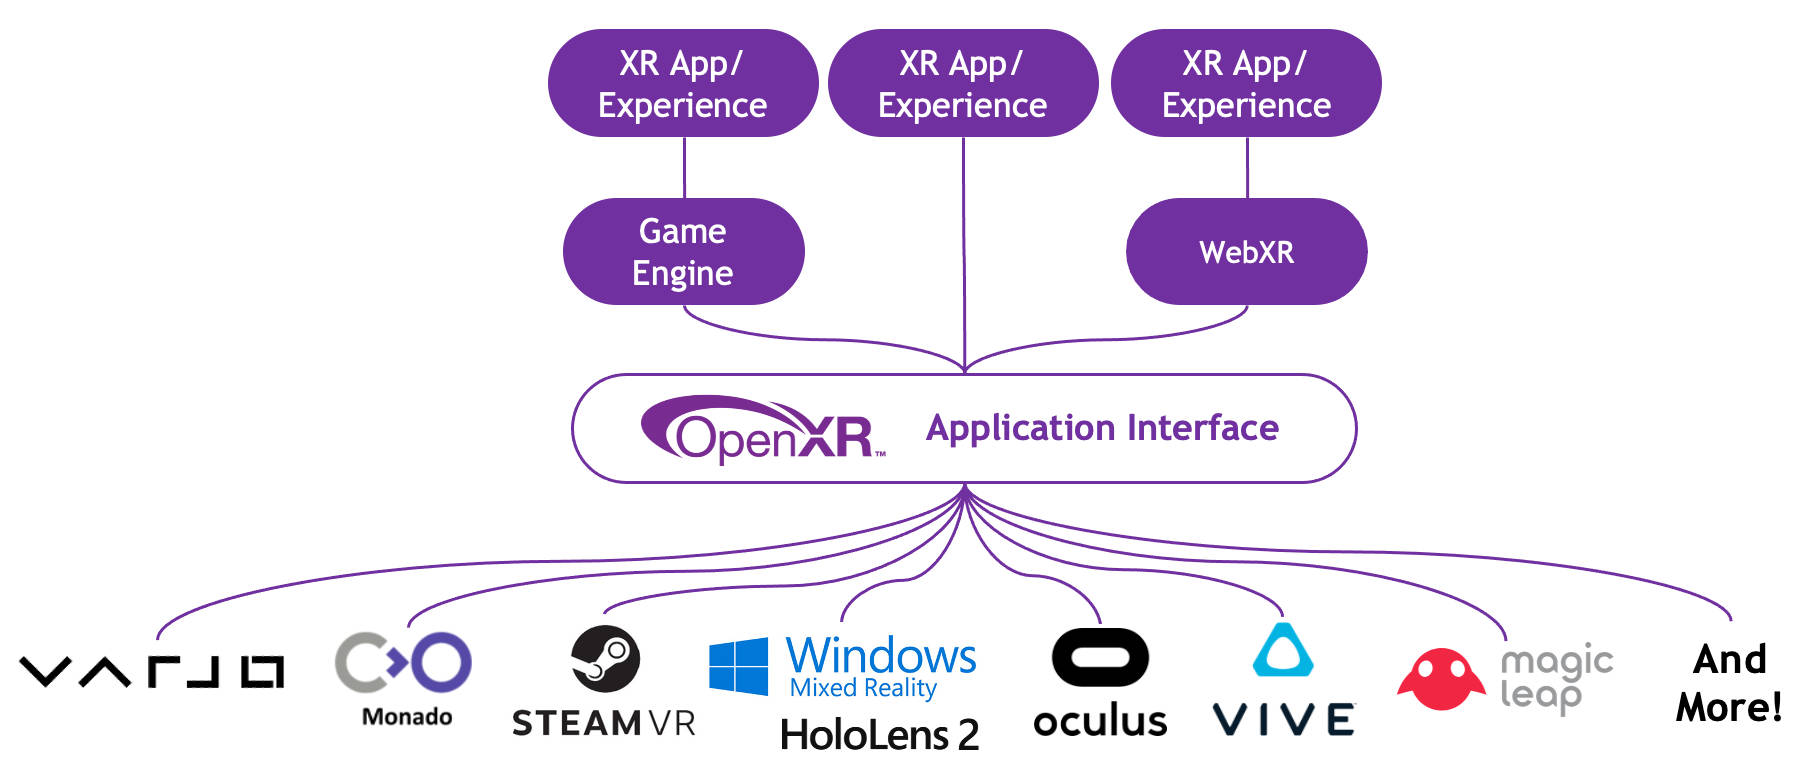
\includegraphics[width=\textwidth]{graphics/openXR-overview.jpg}
    \caption{Overview of the OpenXR API Stack \cite{khronosGroupOpenXR}}
    \label{fig:openxr-overview}
\end{figure}

\section{Prior Publication}
For our implementation we extend the code of a prior publication from Sorger et al. \cite{sorger_immersive_2019}. 
They implemented an immersive visualization for node-link graphs without hierarchical information. Their implementation already contains a common force-based layout, the laser-pointer ray casting technique to select objects, a free flying as well as animated teleport navigation method and lastly a code structure with an included render engine. A screenshot of their work is shown in Figure \ref{fig:priorPublication}.\\
We extended their implementation by adding the ability to visualization hierarchical networks as described in Section \ref{chap:proposed-Solution}. To achieve that we had to adapt the layout algorithm, add transparent rendering, adapt some visual rendering aspects, change the target position for the animated teleport, change the controller button mappings, implement the link filtering technique, add automatic/manual scaling of the virtual scene and automatic/manual adaption of the free flying speed.
This process is described in detail in Section \ref{sec:applOverview} and \ref{sec:applDetails}.

\begin{figure}[!hbt]
    \centering
    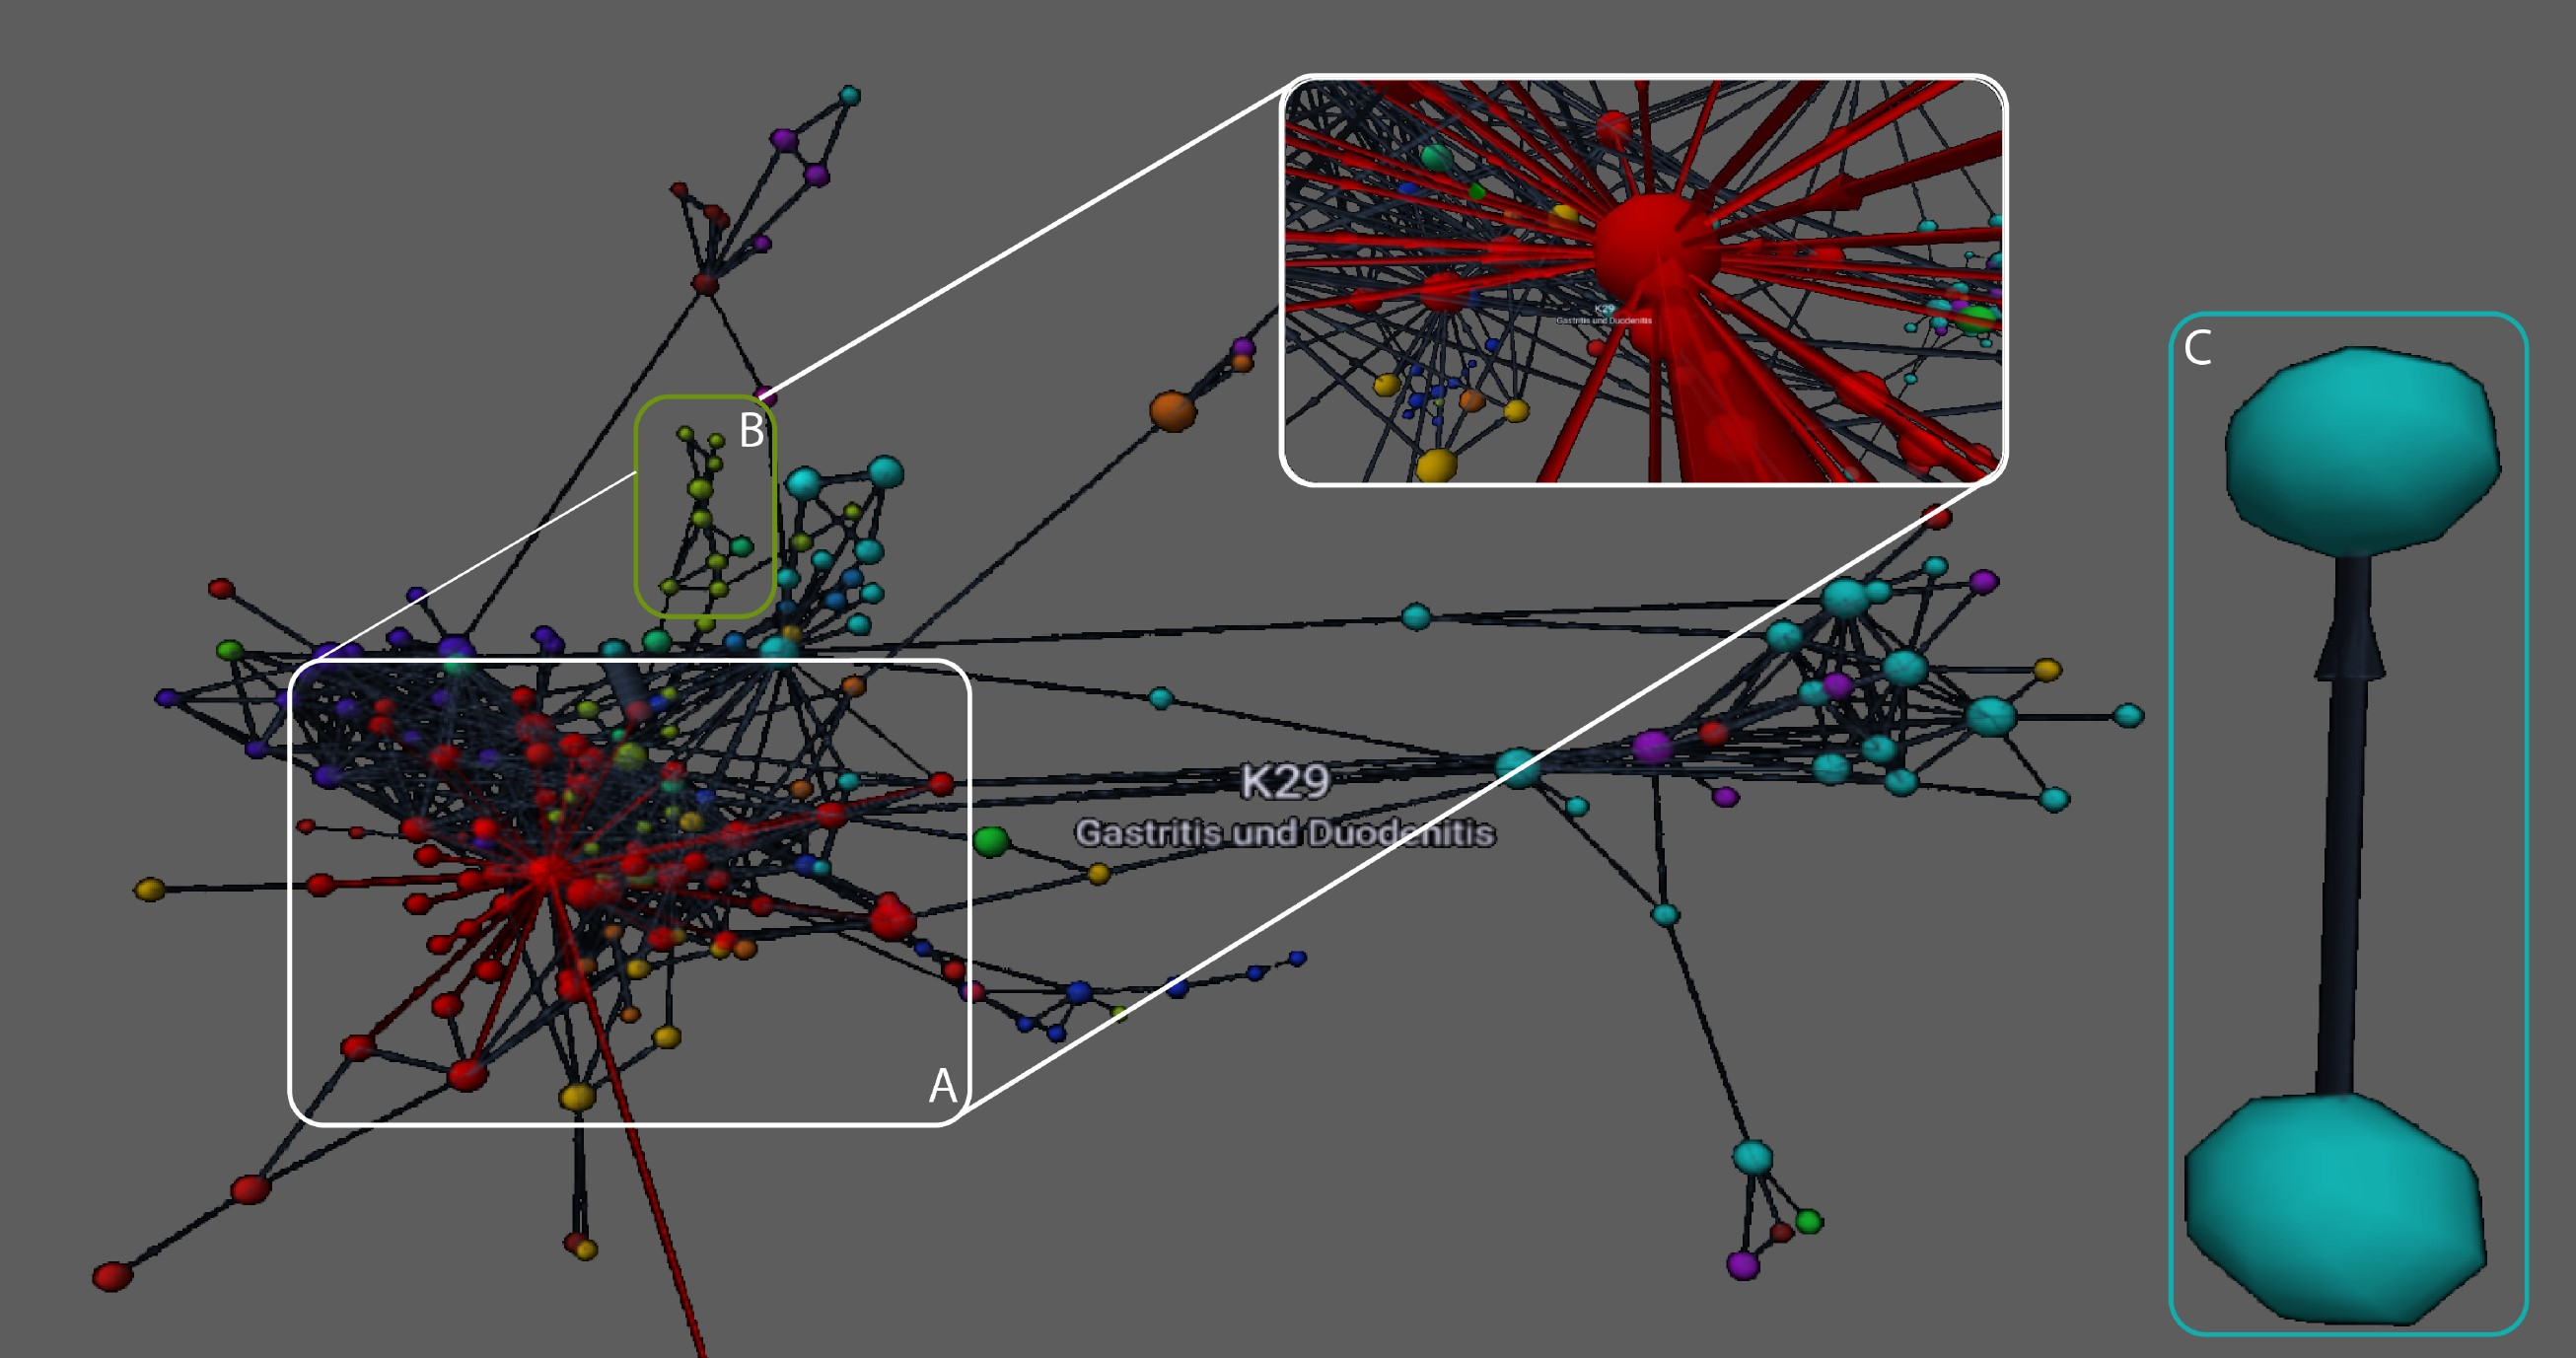
\includegraphics[width=\textwidth]{graphics/screenshotPriorPublication.jpg}
    \caption{Screenshot of the visualization from Sorger et al. \cite{sorger_immersive_2019} we extend our implementation on.}
    \label{fig:priorPublication}
\end{figure}

\section{Technology}

The application is implemented in plain JavaScript and runs in browsers that support the WebVR standard. 
At the time of writing this only applies to Firefox for Windows, our tested version is 85.0.2 (64-Bit). 
WebVR is already deprecated and being replaced with the new WebXR standard, therefore it is unlikely that other browser vendors will implement the standard in the future.\\
In order to reduce the complexity of the rendering and using the WebVR standard the application uses the framework A-Frame \cite{aframe}. A-Frame internally uses three.js \cite{threejs} as a render engine. The code from the publication we extended uses A-Frame in version 0.9.2 from September 2019, this version uses three.js version 0.108.0. 
The old version of A-Frame brings the limitation of only supporting WebVR because WebXR was not yet ready back in 2019. 
Updating A-Frame to a current version that supports WebXR was not possible within a reasonable time therefore we decided to stick to the old version and only support WebVR browsers and headsets.
The primary VR headset we are targeting with our application is the original HTC Vive.

\section{Application Overview}




\label{sec:applOverview}
\subsection{Data Structure}
\label{subSec:dataStruct}
To get a better understanding of the implementation we begin with the data structure for storing the graph.
Listing \ref{lst:internalJSON} shows a minimalistic example of the data structure that we use an input data source. The data is formatted as a JSON object with a flat list of nodes and link. The hierarchical information is encoded with the attributes childNodesIDs and parentNodeID as references. 
In addition to the necessary attributes, each node and link object can have additional attributes depending on the specific dataset.

\begin{lstlisting}[language=json,label={lst:internalJSON},caption=minimal JSON input data structure]
{
    "nodes": [
        {
            "id": "0.0",
            "weight": 4.5,
            "color": "rgb(77, 175, 74)",
            "layer": "0",
            "desc": "0.0",
            "childNodeIDs": [
                "1.1",
                "1.3",
                ...
            ]
        },
        ...
        {
            "id": "1.1",
            "weight": 1.7,
            "color": "rgb(250, 250, 110)",
            "layer": "1",
            "desc": "1.1",
            "parentNodeID": "0.0",
            "childNodeIDs": [
                "2.1",
                ...
            ]
        },
        ...
    ],
    "links": [
        {
            "color": "rgb(77, 175, 74)",
            "layer": "0",
            "source": "0.0",
            "target": "0.1",
            "label": "0.0 - 0.1",
            "linkwidth": 0.35
        },
        ...
    ]
}
\end{lstlisting}

\subsection{Program Flow}
\label{section:programFlow}
\begin{figure}[!hbt]
    \centering
    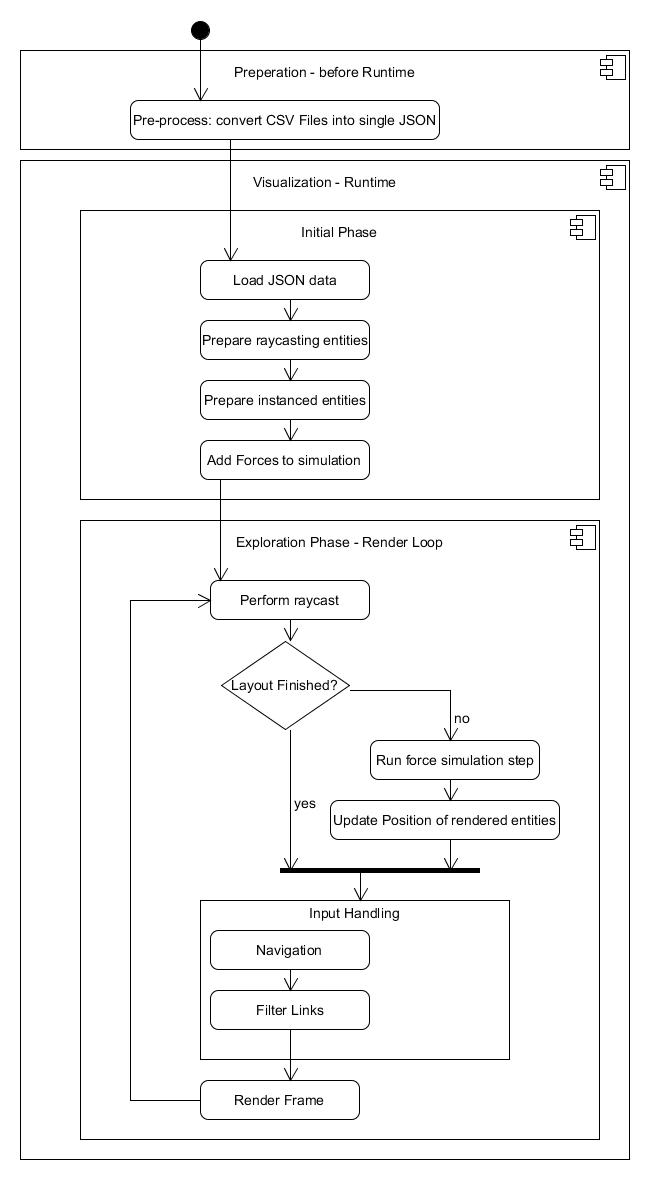
\includegraphics[width=0.74\textwidth]{graphics/vrgraph_flow.jpg}
    \caption{Sequence diagram of the program flow for our application.}
    \label{fig:impl_programFlow}
\end{figure}

We separated the application into multiple processing steps. Figure \ref{fig:impl_programFlow} describes the program flow and all abstract steps that are necessary for the visualization to work.
It contains of an offline preparation phase where the graph data is converted once to our internal JSON data structure (see Section \ref{sec:preprocessing}) and a runtime phase which is executed every time the browser loads the webpage.
After loading the data preparations for the instanced rendering (see Section \ref{sec:rendering}) and the force based layout (see Section \ref{sec:layoutCalculation}) are done.
Then the main render loop is executed which produces a rendered frame for each interaction. In addition, it handles the layout calculation (see Section \ref{sec:layoutCalculation}), navigation and interaction methods (see Section \ref{sec:vrInteractions}), scaling (see Section \ref{sec:scaling}), filtering the graph's links (see Section \ref{sec:linkFiltering}) and performing the ray casting for the virtual laser pointer.
The objects that got intersected by the virtual laser pointer are used in the navigation and interaction techniques. 
Details on how intersected objects are determined by ray casting is not further described as this method is already provided from the original implementation. 

\subsection{Virtual Scene Graph}
A-Frame application are build by creating a virtual scene graph.
It uses an entity-component-system architecture which follows the  composition over inheritance and hierarchy principle. 
This means that every object in A-Frame is an entity that can be customized by code.
There are various components that can be reused and extended, the base component is represented by the <a-entity> element.\\
Listing \ref{lst:virtualSceneGraph} shows a simplified version of the virtual scene graph the application uses. 
It consists of entities for both Vive controllers, a passive and active camera and rig setup and the graph object itself.
Most data and logic is encapsulated in the graphData object. We maintain here two lists of data: a list of nodes/links for the ray casting entities and a list of nodes/links for the actual rendered entities. 
The reason for this duplicated data is that we use  instanced objects for rendering (see Section \ref{sec:rendering}) and these can not be used for ray casting directly.

\begin{lstlisting}[label={lst:virtualSceneGraph},caption=Simplified virtual A-Frame scene graph used by the application.]
<body>
    <a-scene ... >
        <a-entity vive-controls="hand: left"> </a-entity>
        <a-entity vive-controls="hand: right"> </a-entity>
        
        <a-entity id="graphData" json-url="data/inputData.json" ... >
            <a-entity id="passive_rig"  ... >  
                <a-entity id="passive_cam" ... > </a-entity>
            </a-entity>
            ...
        </a-entity>

        <a-entity id="active_rig" ... >
            <a-text id="controllerLabel" ... > </a-text>
            <a-entity id="active_cam" ... > </a-entity>
        </a-entity>
        ...
    </a-scene>
</body>
\end{lstlisting}

\section{Application Details}
\label{sec:applDetails}
\subsection{Preprocessing Scripts}
\label{sec:preprocessing}

The visualization expects a combined JSON file with all nodes and links and their assigned layer as seen in Section \ref{subSec:dataStruct}.
A common data export format for networks are multiple CSV files, one file for the nodes and another for their edges.
In a hierarchical or clustered network there is an additional file with the hierarchical mapping.
Therefore, we needed a script to convert these CSV files to our JSON data format. For convenience most parameters can be configured by an additional config file without changing any program code. 
While transforming the data structure, all node IDs are extended with their hierarchical layer information to ensure unique IDs for the entire dataset.  
In addition, we also normalize the node and link width and add color attributes for a simplified rendering process later on.\\
To test our visualization with various networks of different sizes there is also a script for generating test data available.

\subsection{Layout calculation}
\label{sec:layoutCalculation}
Implementation Details of Forces, \\
Optimization for Saving Pos and set after done

\subsection{Rendering}
\label{sec:rendering}
Goal of Rendering: 
Performance, Support Transparency of nodes. 

Instancing per Links, 
Instancing per Hierarchical Layer of nodes, 
Transparency,
Wireframe

\subsection{VR Interactions}
\label{sec:vrInteractions}

For navigation, we provide two methods free flying and an animated teleport.
Before we go into the details of the technique, it is important to understand the core concept of navigation for 6-DOF VR headsets.\\
The camera is placed in a virtual camera rig which represents the users available movement space (see Figure \ref{fig:vrCameraRig}). 
VR interaction prevent programmatically changing the position of the headset or controllers in the rig. 
The only way the headset and controllers are moved inside the rig is by physical movement in the real world, therefore enable free walking inside the virtual rig.
However, we can programmatically change the position of the rig inside the virtual scene. 
We apply this technique for our free flying and teleport technique.
\begin{figure}[h]
    \centering
    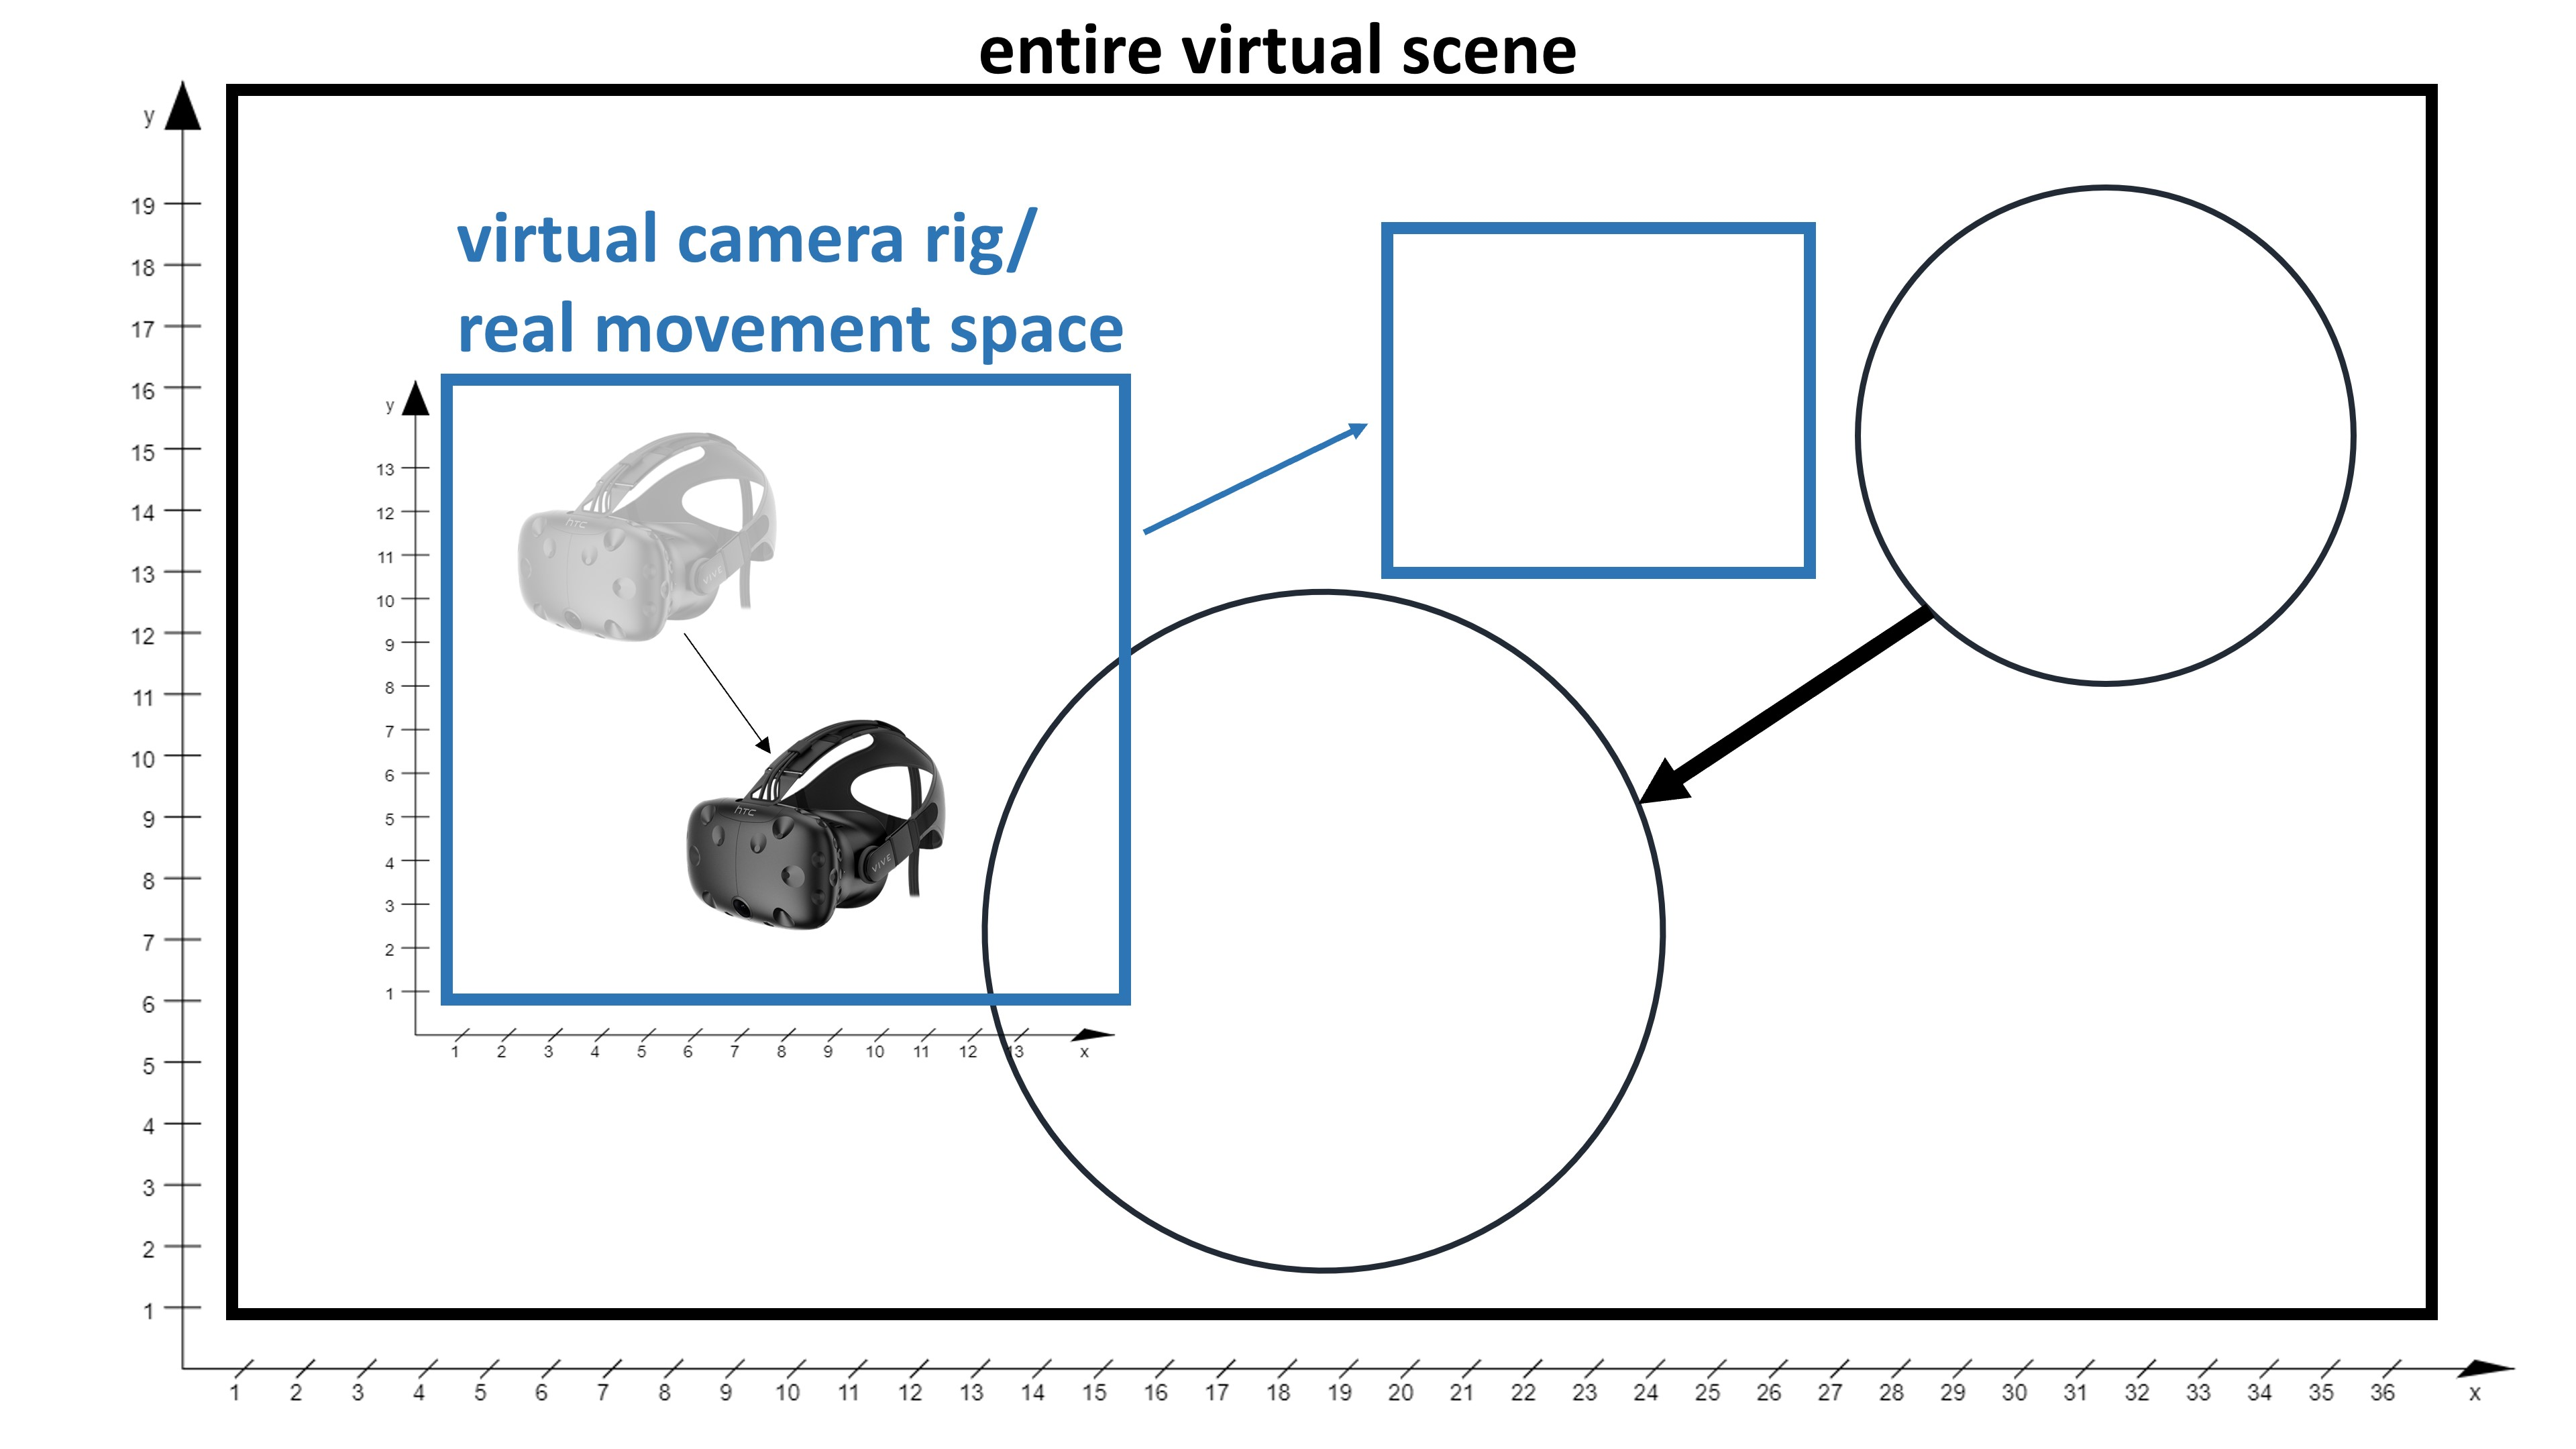
\includegraphics[width=1\textwidth]{graphics/vrCameraRig.jpg}
    \caption{2D representation of the camera rig technique in VR. The scene and rig each have their own coordinates. The headset move around the rig by physical movement and the rig moves around the scene by programmatically navigation methods like free flying or teleportation.} 
    \label{fig:vrCameraRig} 
\end{figure}
\\
The free flying technique is already provided by A-Frame and the implementation from the prior paper.
We just added some additional controller button callbacks for manually selecting the fly speed and rotating the rig in the virtual scene.\\
For the animated teleport technique we adapted the calculation of the target position. The detailed calculating can be seen in Listing \ref{lst:calculationFlyToNode} the process is also visualized in Figure \ref{fig:vrFlyToNode}.

\begin{lstlisting}[language=JavaScript,label={lst:calculationFlyToNode},caption=Matrix calculations for determining the target position of the animated teleport.]
const nodeRadius = multilayerNodeDiameter(node.__data);
const sceneScale = detailLayout.getCurrentSceneScale() ;
let cameraPos = getCurrentCameraRigWorldPos().add(getRelativeCameraToRigPos());
const vecFromNodeToCamera = cameraPos.add(targetPos.clone().negate());
const vectorFromNodeToNodeBorder = vecFromNodeToCamera.normalize().multiplyScalar(nodeRadius*0.95*sceneScale);//*0.95 as we want to be slightly inside the selected node
const positionNodeBorder = targetPos.clone().add(vectorFromNodeToNodeBorder);
const positionNodeBorderCorrectedWithCurrentCameraPos = positionNodeBorder.clone().add(getRelativeCameraToRigPos().negate());
flyToPosition(positionNodeBorderCorrectedWithCurrentCameraPos, flyingElement);
\end{lstlisting}
\begin{figure}[h]
    \centering
    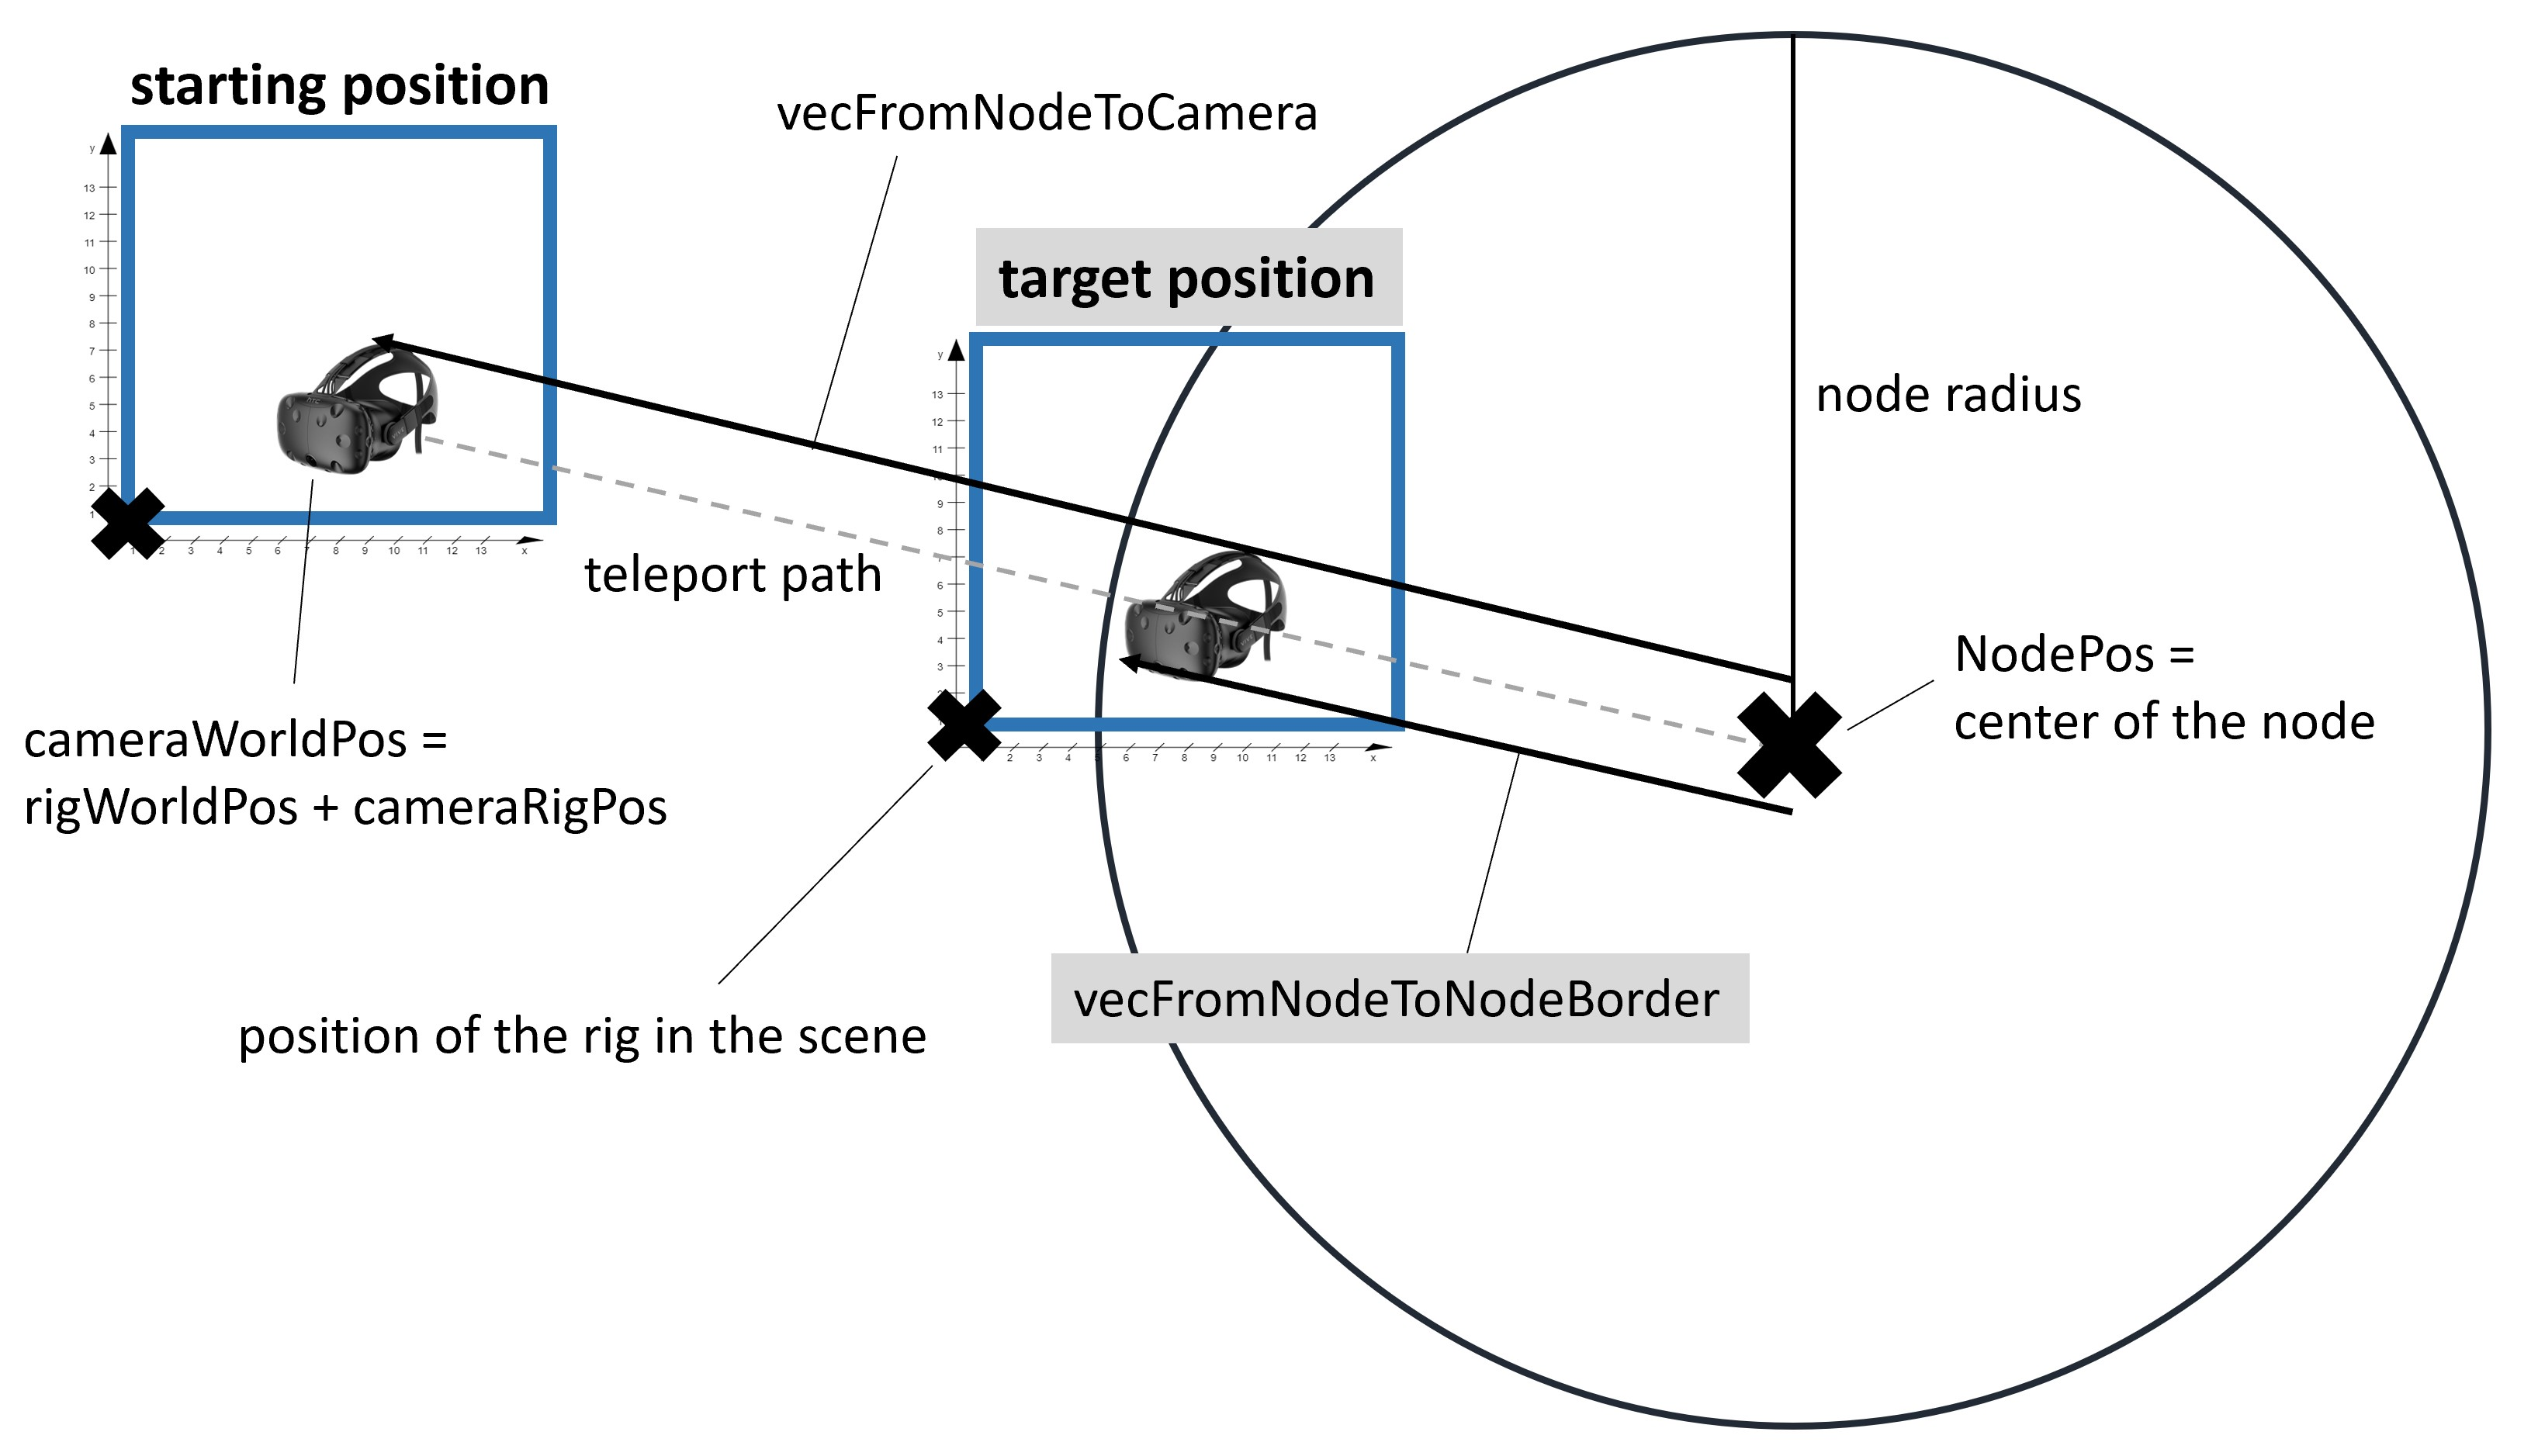
\includegraphics[width=1\textwidth]{graphics/flyToNodePositionCalc.jpg}
    \caption{2D representation of the calculation for the target position for the animated teleport.} 
    \label{fig:vrFlyToNode} 
\end{figure}

Camera Rig vs Camera
camera rotation, correct position 
\\
extend controller
\\
Teleport => calculation of target Position (+Grafik?)
\\
FreeFly

\subsection{Scale}
\label{sec:scaling}

Move + Scale\\
Animation
\\

\subsection{LinkFiltering}
\label{sec:linkFiltering}

Filtering of Links\\
Algorithmus multilayer detail layout\\


\chapter{Results}

\section{Performance}

\subsection{Measurements}

Our setup for the performance tests was a PC with a Ryzen 7 3700X CPU and a Radeon RX 590 GPU.

See Table \ref{table:resultFPS}, See Figure \ref{fig:performanceNodes}, See Figure \ref{fig:performanceLinks}

Notes:
With an increasing number of links the variance of FPS increase. During the animated teleportation the FPS drop noticeably. We assume this is because of the often applied scaling to all entities in the scene. Filtering links does not influence performance. The maximum of 90 FPS is due to the 90HZ panel of the HTC Vive.
CPU and GPU utilization was only about 50\%

\begin{table}
    \centering
    \begin{tabular}{ | c | c | c | c | c | c | }
        \hline
        \textbf{nodes} & \textbf{links} &\textbf{layers} &\textbf{layout - FPS} &\textbf{expl. - min FPS} &\textbf{expl. - avg FPS}\\
        \hline
        310  & 0    & 3 & 40 & 90 & 90\\ \hline
        730  & 0    & 3 & 30 & 70 & 75\\ \hline
        1100 & 0    & 3 & 20 & 55 & 60\\ \hline
        1560 & 0    & 4 & 20 & 40 & 55\\ \hline
        2343 & 0    & 5 & 10 & 30 & 35\\ \hline
        774  & 387  & 3 & 20 & 60 & 70\\ \hline
        774  & 1548 & 3 & 20 & 55 & 70\\ \hline
        774  & 3870 & 3 & 10 & 40 & 60\\ \hline
        1560 & 3120 & 4 & 5  & 25 & 45\\ \hline
        1020 & 2040 & 4 & 10 & 40 & 60\\ \hline
     \end{tabular}
     \caption{Results from performance measurement evaluation(expl. ... exploration).}
     \label{table:resultFPS}
\end{table}


\begin{figure}[h]
    \centering
    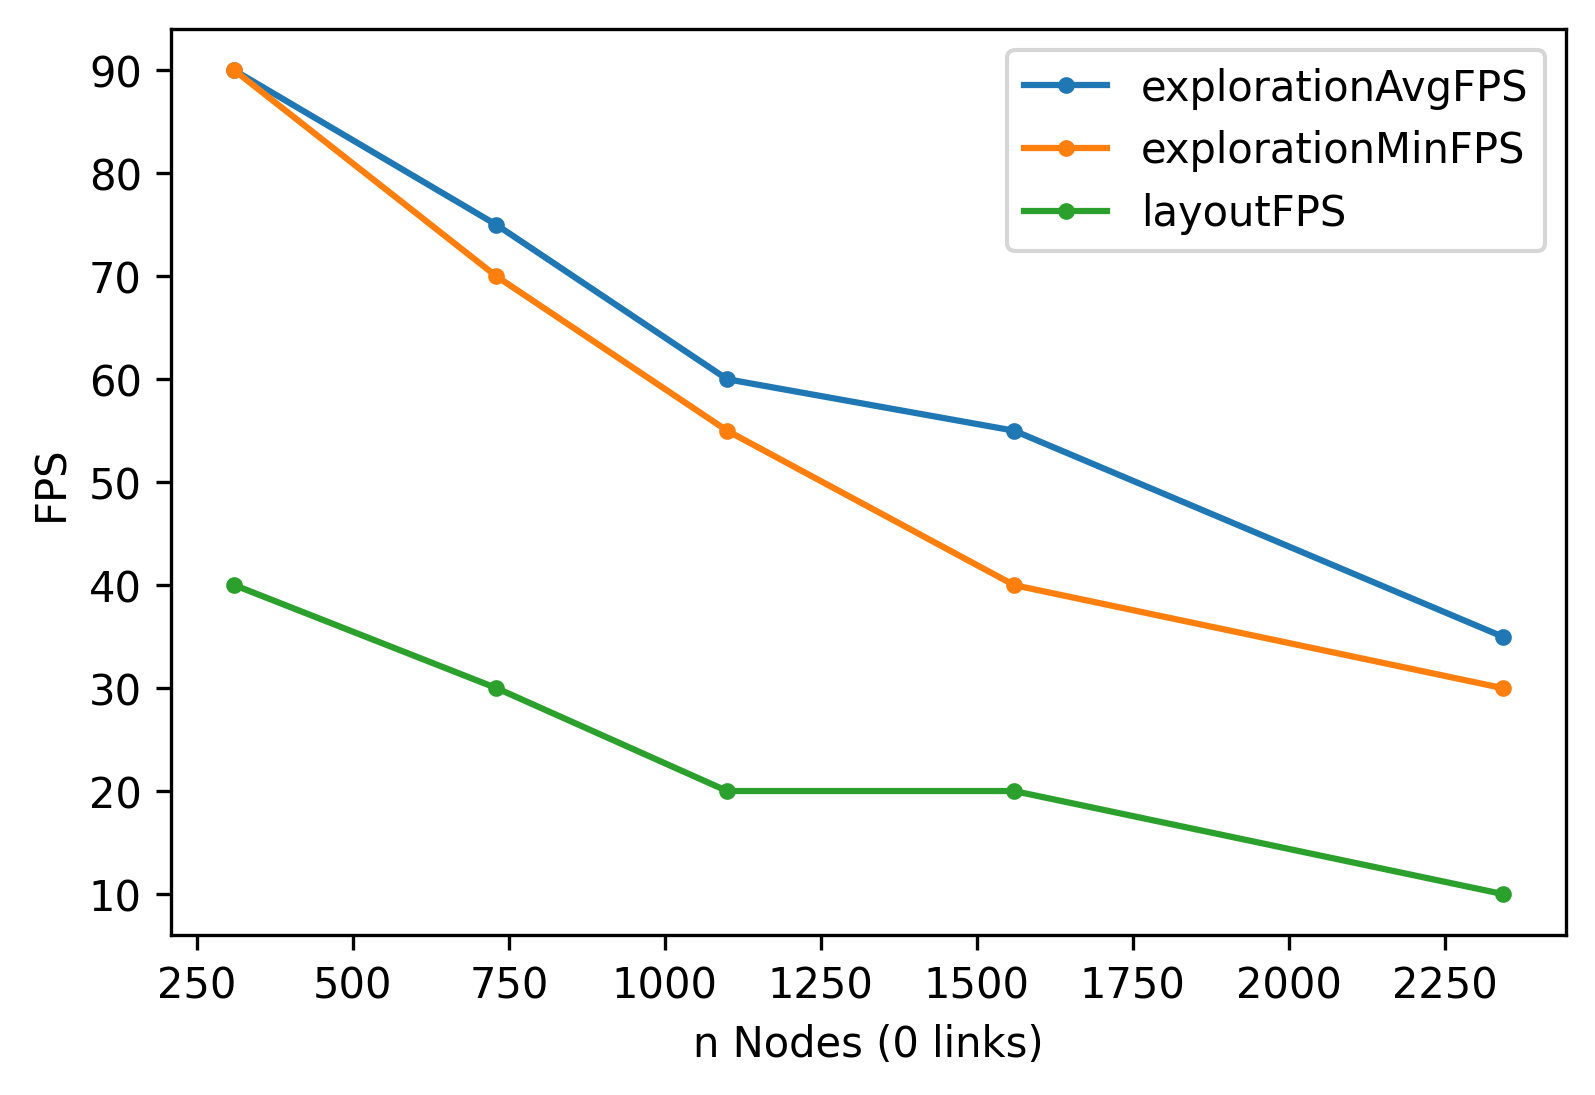
\includegraphics[width=0.75\textwidth]{graphics/performanceAnalysisNodes.png}
    \caption{Performance chart for scaling the number of nodes.} 
    \label{fig:performanceNodes} 
\end{figure}

\begin{figure}[h]
    \centering
    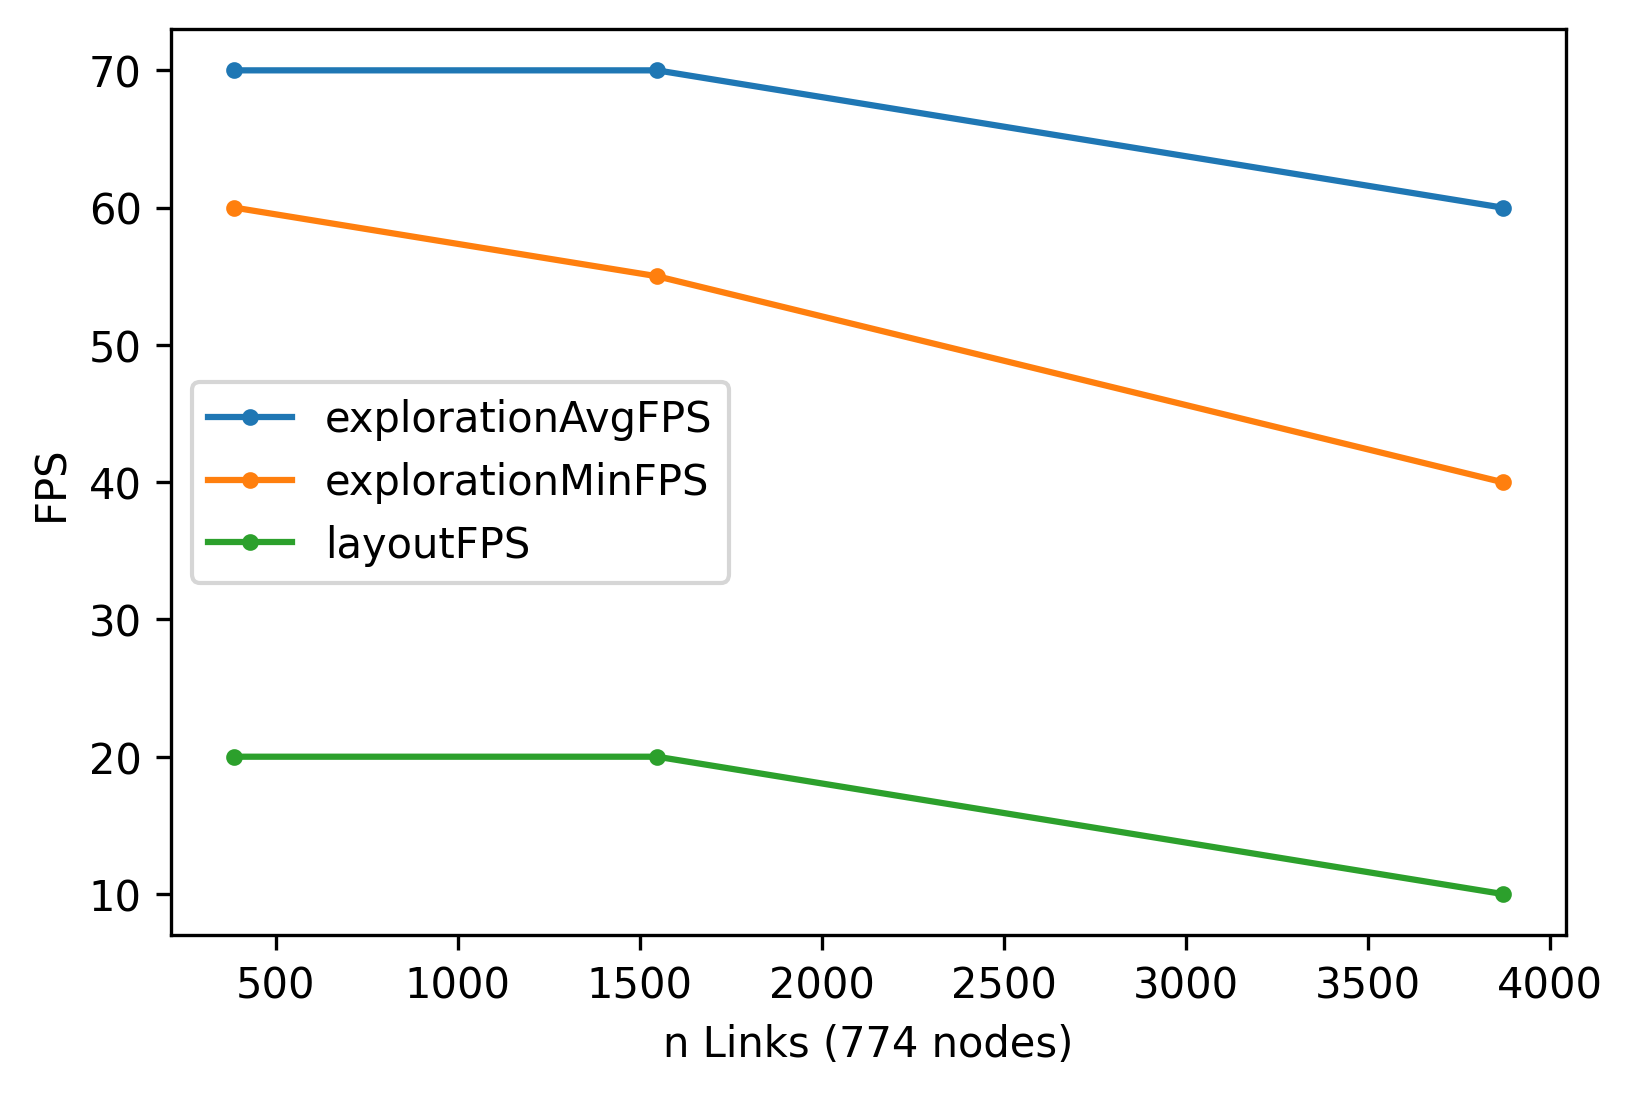
\includegraphics[width=0.75\textwidth]{graphics/performanceAnalysisLinks.png}
    \caption{Performance chart for scaling the number of links.} 
    \label{fig:performanceLinks} 
\end{figure}

\subsection{Possible optimization}

Raycasting only while a button is pressed. 

\section{Informal feedback}

\subsection{Clarity of the visualization}
Filtering, visual clutter, hierarchical layout(intuitive?), ...

\subsection{Navigation}
Free fly, animated teleport, scaling, motion sickness.

\subsection{Interaction}
Button Mappings, Laser Pointer, 

\subsection{Performance}
Tested system and dataset

\chapter{Conclusion and Future Work}

\section{Future Work}
Ideas:
\begin{itemize}
    \item refactor application with the knowledge of the learned mistakes, remove "Aframe-forcegraph-component" as we are not really using any feature now, use a clean dependency management
    \item port to newer version of A-Frame and Three-Js
    \item after upgrading A-Frame version optimize for other VR Headsets, Oculus Quest, ... 
    \item add hand gesture support
    \item optimize data structure (tree data structure  with optimized searched methods)
    \item experiment with different visibility of links/nodes/layers
    \item Add rotate and zoom interaction from paper Embodied Navigation in Immersive Abstract Data Visualization:
    Is Overview+Detail or Zooming Better for 3D Scatterplots?
    \item ...
\end{itemize}


% Remove following line for the final thesis.
%%% intro.tex
%% Copyright (C) 2014-2020 by Thomas Auzinger <thomas@auzinger.name>
%
% This work may be distributed and/or modified under the
% conditions of the LaTeX Project Public License, either version 1.3
% of this license or (at your option) any later version.
% The latest version of this license is in
%   http://www.latex-project.org/lppl.txt
% and version 1.3 or later is part of all distributions of LaTeX
% version 2005/12/01 or later.
%
% This work has the LPPL maintenance status `maintained'.
%
% The Current Maintainer of this work is Thomas Auzinger.
%
% This work consists of the files vutinfth.dtx and vutinfth.ins
% and the derived file vutinfth.cls.
% This work also consists of the file intro.tex.


\newacronym{ctan}{CTAN}{Comprehensive TeX Archive Network}
\newacronym{faq}{FAQ}{Frequently Asked Questions}
\newacronym{pdf}{PDF}{Portable Document Format}
\newacronym{svn}{SVN}{Subversion}
\newacronym{wysiwyg}{WYSIWYG}{What You See Is What You Get}

\newglossaryentry{texteditor}
{
  name={editor},
  description={A text editor is a type of program used for editing plain text files.}
}

\chapter{Introduction to \LaTeX}

Since \LaTeX\ is widely used in academia and industry, there exists a plethora of freely accessible introductions to the language.
Reading through the guide at \url{https://en.wikibooks.org/wiki/LaTeX} serves as a comprehensive overview for most of the functionality and is highly recommended before starting with a thesis in \LaTeX.

\section{Installation}

A full \LaTeX\ distribution\index{distribution} consists not only of the binaries that convert the source files to the typeset documents, but also of a wide range of packages and their documentation.
Depending on the operating system, different implementations are available as shown in Table~\ref{tab:distrib}.
\textbf{Due to the large amount of packages that are in everyday use and due to their high interdependence, it is paramount to keep the installed distribution\index{distribution} up to date.}
Otherwise, obscure errors and tedious debugging ensue.

\begin{table}
  \centering
  \begin{tabular}{cccc}
    \toprule
    Distribution & Unix         & Windows      & MacOS        \\
    \midrule
    TeX Live     & \textbf{yes} & yes          & (yes)        \\
    MacTeX       & no           & no           & \textbf{yes} \\
    MikTeX       & (yes)        & \textbf{yes} & yes          \\
    \bottomrule
  \end{tabular}
  \caption{\TeX/\LaTeX\ distributions for different operating systems. Recomended choice in \textbf{bold}.}
  \label{tab:distrib} % \label has to be placed AFTER \caption to produce correct cross-references.
\end{table}

\section{Editors}

A multitude of \TeX\ \glspl{texteditor} are available differing in their editing models, their supported operating systems and their feature sets.
A comprehensive overview of \glspl{texteditor} can be found at the Wikipedia page  \url{https://en.wikipedia.org/wiki/Comparison_of_TeX_editors}.
TeXstudio (\url{http://texstudio.sourceforge.net/}) is recommended.
Most editors support a synchronization of the generated document and the \LaTeX\ source by \verb|Ctrl| clicking either on the source document or the generated document.

\section{Compilation}

Modern editors usually provide the compilation programs to generate \gls{pdf} documents and for most \LaTeX\ source files, this is sufficient.
More advanced \LaTeX\ functionality, such as glossaries and bibliographies, needs additional compilation steps, however.
It is also possible that errors in the compilation process invalidate intermediate files and force subsequent compilation runs to fail.
It is advisable to delete intermediate files (\verb|.aux|, \verb|.bbl|, etc.), if errors occur and persist.
All files that are not generated by the user are automatically regenerated.
To compile the current document, the steps as shown in Table~\ref{tab:compile} have to be taken.


\begin{table}
  \centering
  \begin{tabular}{rl}
    \toprule
    & Description \\
    \midrule
    1 & Scan for refs, toc/lof/lot/loa items and cites \\
    2 & Build the bibliography     \\
    3 & Link refs and build the toc/lof/lot/loa \\
    4 & Link the bibliography \\
    5 & Build the glossary \\
    6 & Build the acronyms \\
    7 & Build the index \\
    8 & Link the glossary, acronyms, and the index \\
    9 & Link the bookmarks \\
    \midrule
    & Command \\
    \midrule
    1 & \verb|pdflatex.exe  example| \\
    2 & \verb|bibtex.exe    example| \\
    3 & \verb|pdflatex.exe  example| \\
    4 & \verb|pdflatex.exe  example| \\
    5 & \verb|makeindex.exe -t example.glg -s example.ist| \\
      & \verb|              -o example.gls example.glo| \\
    6 & \verb|makeindex.exe -t example.alg -s example.ist| \\
      & \verb|              -o example.acr example.acn| \\
    7 & \verb|makeindex.exe -t example.ilg -o example.ind example.idx| \\
    8 & \verb|pdflatex.exe  example| \\
    9 & \verb|pdflatex.exe  example| \\
    \bottomrule
  \end{tabular}
  \caption{Compilation steps for this document. The following abbreviations were used: table of contents (toc), list of figures (lof), list of tables (lot), list of algorithms (loa).}
  \label{tab:compile} % \label has to be placed AFTER \caption to produce correct cross-references.
\end{table}


\section{Basic Functionality}

In this section, various examples are given of the fundamental building blocks used in a thesis.
Many \LaTeX\ commands have a rich set of options that can be supplied as optional arguments.
The documentation of each command should be consulted to get an impression of the full spectrum of its functionality.

\subsection{Floats}

Two main categories of page elements can be differentiated in the usual \LaTeX\ workflow: \textit{(i)} the main stream of text and \textit{(ii)} floating containers that are positioned at convenient positions throughout the document.
In most cases, tables, plots, and images are put into such containers since they are usually positioned at the top or bottom of pages.
These are realized by the two environments \verb|figure| and \verb|table|, which also provide functionality for cross-referencing (see Table~\ref{tab:intro} and Figure~\ref{fig:intro}) and the generation of corresponding entries in the list of figures and the list of tables.
Note that these environments solely act as containers and can be assigned arbitrary content.

\subsection{Tables}

A table in \LaTeX\ is created by using a \verb|tabular| environment or any of its extensions, e.g., \verb|tabularx|.
The commands \verb|\multirow| and \verb|\multicolumn| allow table elements to span multiple rows and columns.

\begin{table}[h] % placement specifier
  \centering
  \begin{tabular}{lll}
    \toprule
    \multicolumn{2}{c}{Position} \\
    \cmidrule{1-2} % partial horizontal rule
    Group & Abbrev & Name \\
    \midrule
    Goalkeeper & GK & Paul Robinson \\
    \midrule
    \multirow{4}{*}{Defenders} & LB & Lucus Radebe \\
                               & DC & Michael Duburry \\
                               & DC & Dominic Matteo \\
                               & RB & Didier Domi \\
    \midrule
    \multirow{3}{*}{Midfielders} & MC & David Batty \\
                                 & MC & Eirik Bakke \\
                                 & MC & Jody Morris \\
    \midrule
    Forward & FW & Jamie McMaster \\
    \midrule
    \multirow{2}{*}{Strikers} & ST & Alan Smith \\
                              & ST & Mark Viduka \\
    \bottomrule
  \end{tabular}
  \caption{Adapted example from the \LaTeX guide at \url{https://en.wikibooks.org/wiki/LaTeX/Tables}. This example uses rules specific to the \texttt{booktabs} package and employs the multi-row functionality of the \texttt{multirow} package.}
  \label{tab:intro} % \label has to be placed AFTER \caption to produce correct cross-references.
\end{table}

\subsection{Images}

An image is added to a document via the \verb|\includegraphics| command as shown in Figure~\ref{fig:intro}.
The \verb|\subcaption| command can be used to reference subfigures, such as Figure~\ref{fig:intro:full width} and~\ref{fig:intro:half width}.

\begin{figure}[h]
  \centering
  \begin{subfigure}[b]{0.45\columnwidth}
    \centering
    
\includegraphics[width=\textwidth]{Logo-schwarz.pdf}
    \subcaption{The header logo at text width.}
    \label{fig:intro:full width}
  \end{subfigure}
  \begin{subfigure}[b]{0.45\columnwidth}
    \centering
    
\includegraphics[width=0.5\textwidth]{Logo-schwarz.pdf}
    \subcaption{The header logo at half the text width.}
    \label{fig:intro:half width}
  \end{subfigure}
  \caption[Optional caption for the figure list (often used to abbreviate long captions)]{The header logo at different sizes.} % Remove the [...] argument if the original caption should be used in the figure list.
  \label{fig:intro} % \label has to be placed AFTER \caption (or \subcaption) to produce correct cross-references.
\end{figure}

\subsection{Mathematical Expressions}

One of the original motivation to create the \TeX\ system was the need for mathematical typesetting.
To this day, \LaTeX\ is the preferred system to write math-heavy documents and a wide variety of functions aids the author in this task.
A mathematical expression can be inserted inline as $\sum_{n=1}^{\infty} \frac{1}{n^2} = \frac{\pi^2}{6}$ outside of the text stream as \[ \sum_{n=1}^{\infty} \frac{1}{n^2} = \frac{\pi^2}{6} \] or as numbered equation with
\begin{equation}
\sum_{n=1}^{\infty} \frac{1}{n^2} = \frac{\pi^2}{6}.
\end{equation}

\subsection{Pseudo Code}

The presentation of algorithms can be achieved with various packages; the most popular are \verb|algorithmic|, \verb|algorithm2e|, \verb|algorithmicx|, or \verb|algpseudocode|.
An overview is given at \url{https://tex.stackexchange.com/questions/229355}.
An example of the use of the \verb|alogrithm2e| package is given with Algorithm~\ref{alg:gauss-seidel}.

\begin{algorithm}
  \SetKw{BreakFor}{break for}
  \KwIn{A scalar~$\epsilon$, a matrix $\mathbf{A} = (a_{ij})$, a vector $\vec{b}$, and an initial vector $\vec{x}^{(0)}$}
  \KwOut{$\vec{x}^{(n)}$ with $\mathbf{A} \vec{x}^{(n)} \approx \vec{b}$}
  \For{$k\leftarrow 1$ \KwTo maximum iterations}
  {
     \For{$i\leftarrow 1$ \KwTo $n$}
     {
        $x_i^{(k)} = \frac{1}{a_{ii}} \left(b_i-\sum_{j<i} a_{ij} x_j^{(k)} - \sum_{j>i} a_{ij} x_j^{(k-1)} \right)$\;
     }
     \If{$\lvert\vec{x}^{(k)}-\vec{x}^{(k-1)}\rvert < \epsilon$}
     {\BreakFor\;}
  }
  \Return{$\vec{x}^{(k)}$\;}
  \caption{Gauss-Seidel}
  \label{alg:gauss-seidel} % \label has to be placed AFTER \caption to produce correct cross-references.
\end{algorithm}

\section{Bibliography}

The referencing of prior work is a fundamental requirement of academic writing and well supported by \LaTeX.
The \textsc{Bib}\TeX\ reference management software is the most commonly used system for this purpose.
Using the \verb|\cite| command, it is possible to reference entries in a \verb|.bib| file out of the text stream, e.g., as~\cite{Turing1936}.
The generation of the formatted bibliography needs a separate execution of \verb|bibtex.exe| (see Table~\ref{tab:compile}).

\section{Table of Contents}

The table of contents is automatically built by successive runs of the compilation, e.g., of \verb|pdflatex.exe|.
The command \verb|\setsecnumdepth| allows the specification of the depth of the table of contents and additional entries can be added to the table of contents using \verb|\addcontentsline|.
The starred versions of the sectioning commands, i.e., \verb|\chapter*|, \verb|\section*|, etc., remove the corresponding entry from the table of contents.

\section{Acronyms / Glossary / Index}

The list of acronyms, the glossary, and the index need to be built with a separate execution of \verb|makeindex| (see Table~\ref{tab:compile}).
Acronyms have to be specified with \verb|\newacronym| while glossary entries use \verb|\newglossaryentry|.
Both are then used in the document content with one of the variants of \verb|\gls|, such as \verb|\Gls|, \verb|\glspl|, or \verb|\Glspl|.
Index items are simply generated by placing \verb|\index|\marg{entry} next to all the words that correspond to the index entry \meta{entry}.
Note that many enhancements exist for these functionalities and the documentation of the \verb|makeindex| and the \verb|glossaries| packages should be consulted.

\section{Tips}

Since \TeX\ and its successors do not employ a \gls{wysiwyg} editing scheme, several guidelines improve the readability of the source content:
\begin{itemize}
\item Each sentence in the source text should start with a new line.
      This helps not only the user navigation through the text, but also enables revision control systems (e.g. \gls{svn}, Git) to show the exact changes authored by different users.
      Paragraphs are separated by one (or more) empty lines.
\item Environments, which are defined by a matching pair of \verb|\begin{name}| and \verb|\end{name}|, can be indented by whitespace to show their hierarchical structure.
\item In most cases, the explicit use of whitespace (e.g. by adding \verb|\hspace{4em}| or \verb|\vspace{1.5cm}|) violates typographic guidelines and rules.
      Explicit formatting should only be employed as a last resort and, most likely, better ways to achieve the desired layout can be found by a quick web search.
\item The use of bold or italic text is generally not supported by typographic considerations and the semantically meaningful \verb|\emph{|\texttt{$\dots$}\verb|}| should be used.
\end{itemize}

The predominant application of the \LaTeX\ system is the generation of \gls{pdf} files via the \textsc{Pdf}\LaTeX\ binaries.
In the current version of \textsc{Pdf}\LaTeX, it is possible that absolute file paths and user account names are embedded in the final \gls{pdf} document.
While this poses only a minor security issue for all documents, it is highly problematic for double blind reviews.
The process shown in Table~\ref{tab:ps2pdf} can be employed to strip all private information from the final \gls{pdf} document.

\begin{table}[h]
  \centering
  \begin{tabular}{rl}
  \toprule
  & Command \\
  \midrule
  1 & Rename the \gls{pdf} document \verb|final.pdf| to \verb|final.ps|. \\
  2 & Execute the following command: \\
    & \verb|ps2pdf -dPDFSETTINGS#/prepress ^| \\
    & \verb| -dCompatibilityLevel#1.4 ^| \\
    & \verb| -dAutoFilterColorImages#false ^| \\
    & \verb| -dAutoFilterGrayImages#false ^| \\
    & \verb| -dColorImageFilter#/FlateEncode ^| \\
    & \verb| -dGrayImageFilter#/FlateEncode ^| \\
    & \verb| -dMonoImageFilter#/FlateEncode ^| \\
    & \verb| -dDownsampleColorImages#false ^| \\
    & \verb| -dDownsampleGrayImages#false ^| \\
    & \verb| final.ps final.pdf| \\
  \bottomrule
  \end{tabular}

  On Unix-based systems, replace \verb|#| with \verb|=| and \verb|^| with \verb|\|.
  \caption{Anonymization of \gls{pdf} documents.}
  \label{tab:ps2pdf}
\end{table}

\section{Resources}

\subsection{Useful Links}

In the following, a listing of useful web resources is given.
\begin{description}
\item[\url{https://en.wikibooks.org/wiki/LaTeX}] An extensive wiki-based guide to \LaTeX.
\item[\url{http://www.tex.ac.uk/faq}] A (huge) set of \gls{faq} about \TeX\ and \LaTeX.
\item[\url{https://tex.stackexchange.com/}] The definitive user forum for non-trivial \LaTeX-related questions and answers.
\end{description}

\subsection[Comprehensive TeX Archive Network]{\gls{ctan}}

The \gls{ctan} is the official repository for all \TeX\ related material.
It can be accessed via \url{https://www.ctan.org/} and hosts (among other things) a huge variety of packages that provide extended functionality for \TeX\ and its successors.
Note that most packages contain \gls{pdf} documentation that can be directly accessed via \gls{ctan}.

In the following, a short, non-exhaustive list of relevant \gls{ctan}-hosted packages is given together with their relative path.
\begin{description}[itemsep=0ex]
\item[\href{https://www.ctan.org/pkg/algorithm2e}{algorithm2e}] Functionality for writing pseudo code.
\item[\href{https://www.ctan.org/pkg/amsmath}{amsmath}] Enhanced functionality for typesetting mathematical expressions.
\item[\href{https://www.ctan.org/pkg/amsfonts}{amssymb}] Provides a multitude of mathematical symbols.
\item[\href{https://www.ctan.org/pkg/booktabs}{booktabs}] Improved typesetting of tables.
\item[\href{https://www.ctan.org/pkg/enumitem}{enumitem}] Control over the layout of lists (\verb|itemize|, \verb|enumerate|, \verb|description|).
\item[\href{https://www.ctan.org/pkg/fontenc}{fontenc}] Determines font encoding of the output.
\item[\href{https://www.ctan.org/pkg/glossaries}{glossaries}] Create glossaries and list of acronyms.
\item[\href{https://www.ctan.org/pkg/graphicx}{graphicx}] Insert images into the document.
\item[\href{https://www.ctan.org/pkg/inputenc}{inputenc}] Determines encoding of the input.
\item[\href{https://www.ctan.org/pkg/l2tabu}{l2tabu}] A description of bad practices when using \LaTeX.
\item[\href{https://www.ctan.org/pkg/mathtools}{mathtools}] Further extension of mathematical typesetting.
\item[\href{https://www.ctan.org/pkg/memoir}{memoir}] The document class on upon which the \verb|vutinfth| document class is based.
\item[\href{https://www.ctan.org/pkg/multirow}{multirow}] Allows table elements to span several rows.
\item[\href{https://www.ctan.org/pkg/pgfplots}{pgfplots}] Function plot drawings.
\item[\href{https://www.ctan.org/pkg/pgf}{pgf/TikZ}] Creating graphics inside \LaTeX\ documents.
\item[\href{https://www.ctan.org/pkg/subcaption}{subcaption}] Allows the use of subfigures and enables their referencing.
\item[\href{https://www.ctan.org/tex-archive/info/symbols/comprehensive/}{symbols/comprehensive}] A listing of around 5000 symbols that can be used with \LaTeX.
\item[\href{https://www.ctan.org/pkg/voss-mathmode}{voss-mathmode}] A comprehensive overview of typesetting mathematics in \LaTeX.
\item[\href{https://www.ctan.org/pkg/xcolor}{xcolor}] Allows the definition and use of colors.
\end{description} % A short introduction to LaTeX.

\backmatter

% Use an optional list of figures.
\listoffigures % Starred version, i.e., \listoffigures*, removes the toc entry.

% Use an optional list of tables.
\cleardoublepage % Start list of tables on the next empty right hand page.
\listoftables % Starred version, i.e., \listoftables*, removes the toc entry.

% Use an optional list of alogrithms.
%\listofalgorithms
%\addcontentsline{toc}{chapter}{List of Algorithms}

% Add an index.
\printindex

% Add a glossary.
\printglossaries

% Add a bibliography.
\bibliographystyle{alpha}
\bibliography{intro}

\end{document}